%%%%%%%%%%%%%%%%%%%%%%%%%%%%%%%%%%%%%%%%%%%%%%%%%%%%%%%%%%%%%%%%%%%%%%%%%%%%%%%
%                                                                             %
%           TEMPLATE LATEX PER TESI                                           %
%           ______________                                                    %
%                                                                             %
%           Ultima revisione: 10 Dicembre 2025                                %
%           Revisori: G.Presti; L.A.Ludovico; F. Avanzini; M. Tiraboschi      %
%                                                                             %
%%%%%%%%%%%%%%%%%%%%%%%%%%%%%%%%%%%%%%%%%%%%%%%%%%%%%%%%%%%%%%%%%%%%%%%%%%%%%%%

% Usare l'opzione twoside se volete stampare fronte-retro. Es.:
% \documentclass[twoside,12pt]{report}
% Si consiglia di diminuire il font per tesi di dottorato in formato 17x24. Es:
% \documentclass[11pt]{report}
\documentclass[12pt]{report}

% --- PREAMBOLO ---------------------------------------------------------------
% Inserire qui eventuali package da includere o 
% definizioni di comandi personalizzati...

% ...ad esempio il seguente package permette di inserire note visibili nel pdf di output,
% (il comando che lo precede serve a lasciare spazio alle note, va rimosso prima della consegna)
% \setlength {\marginparwidth }{2cm}
% \usepackage{todonotes}  % istruzioni sull'uso in sezione 3.2.9

% Selezione lingua
\usepackage[italian]{babel}

\usepackage{siunitx}
\usepackage{graphicx}
\usepackage{subcaption}
\usepackage{listings}
\usepackage{xcolor}

\lstdefinelanguage{json}{
	basicstyle=\ttfamily\small,
	numbers=left,
	numberstyle=\tiny\color{gray},
	stepnumber=1,
	numbersep=8pt,
	showstringspaces=false,
	breaklines=true,
	frame=single,
	string=[s]{"}{"},
	stringstyle=\color{blue},
	comment=[l]{:},
	commentstyle=\color{black},
}
\lstdefinestyle{pythonstyle}{
	language=Python,
	basicstyle=\ttfamily\small,
	numbers=left,
	numberstyle=\tiny\color{gray},
	keywordstyle=\color{blue},
	commentstyle=\color{green!50!black},
	stringstyle=\color{red!70!black},
	showstringspaces=false,
	breaklines=true,
	frame=single,
	tabsize=4,
	keepspaces=true
}

\lstset{
	tabsize=2,
	keepspaces=true
}

\usepackage{tesi}
% Puoi usare il font di default di LaTeX con la relativa opzione del package
% \usepackage[defaultfont]{tesi}
% Esiste anche un'opzione per il formato 17x24 per le tesi di dottorato
% \usepackage[phd]{tesi}

% In caso il copia-incolla del PDF generato perda gli spazi,
% provare a decommentare la seguente riga
% \pdfinterwordspaceon

% !!! INFORMAZIONI SULLA TESI DA COMPILARE !!!

%   UNIVERSITA' E CORSO DI LAUREA:
\university{Università degli Studi di Milano}
\unilogo{immagini/loghi/unimi}
\faculty{Facoltà di Scienze e Tecnologie}
\department{Dipartimento di Informatica\\Giovanni Degli Antoni}
\cdl{Corso di Laurea Triennale in\\Informatica}

%   TITOLO TESI:
\title{Studio e realizzazione di un drone a volo autonomo in assenza di geolocalizzazione}

%   AUTORE:
\author{Filippo Raciti}
\matricola{29692A}
% "Elaborato Finale" per i CdL triennali
% "Tesi di Laurea" per i CdL magistrali
\typeofthesis{Elaborato Finale}

%   RELATORE E CORRELATORE:
\relatore{Prof. Federico Pedersini}
\correlatore{Prof. Giorgio Biacchi}

%   LABORATORIO:
% Questa sezione crea una pagina di chiusura della tesi con
% il logo dell'ente/laboratorio presso cui si è svolto il tirocinio.
% Più afferenze/url/loghi sono supportate,
% e la frase può essere personalizzata.
% Qui trovate alcuni predefiniti del nostro dipartimento
% \adaptlab
% \aislab
% \anacletolab
% \bisplab
% \connetslab
% \everywarelab
% \falselab
% \iebilab
% \islab
% \lailalab
% \lalalab
% \lawlab
% \laserlab
% \limlab
% \mipslab
% \optlab
% \phuselab
% \ponglab
% \sesarlab
% \spdplab

% Esempio di personalizzazione della pagina di chiusura
% (non consegnate con questo esempio!)
% (da commentare in caso sia sufficiente una delle macro precedenti)
% \lab{Laboratorio di Ricerca}
% \lab[in collaborazione con l']{Azienda Specifica}
% \laburl{https://di.unimi.it/it/ricerca/risorse-e-luoghi-della-ricerca/laboratori-di-ricerca}
% \lablogo{immagini/redqmark}

% Con questo comando si può cambiare la dimensione (massima
% altezza e larghezza consentite) dei loghi
% \setlength\lablogosize{25mm}

%   ANNO ACCADEMICO
% \the\year inserisce l'anno corrente
% per specificare manualmente un anno accademico
% NON inserire nel formato 1970-1971, ma
% inserire solo 1970
\academicyear{2025} 

%   INDICI:
% elenco delle figure (facoltativo)
% \figurespagetrue
% elenco delle tabelle (facoltativo)
% \tablespagetrue
% prefazioni nell'indice (facoltativo)
\prefaceintoctrue
% indice nell'indice (facoltativo)
\tocintoctrue
% --- FINE PREAMBOLO ----------------------------------------------------------

\begin{document}

% Creazione automatica della copertina
% Centra la copertina nel foglio: usa questo comando per la copertina esterna
% \makecenteredfrontpage
% Copertina allineata alle altre pagine: usa questo comando per la copertina interna
\makefrontpage

% 
%			PAGINA DI DEDICA E/O CITAZIONE
%			facoltativa, questa è l'unica cosa che dovete formattare a mano, un po' come vi pare
%

% {...}

% \clearpage
% \beforepreface

% 
%			PREFAZIONE (facoltativa)
%

% \prefacesection{Prefazione}
% Le prefazioni non sono molto comuni, tuttavia a volte capita che qualcuno voglia dire qualcosa che esuli dal lavoro in sé (come un meta-commento sull'elaborato), o voglia fornire informazioni riguardanti l'eventuale progetto entro cui la tesi si colloca (in questo caso è probabile che sia il relatore a scrivere questa parte).

%
%			SOMMARIO
%

\prefacesection{Sommario}
%La localizzazione è un aspetto in robotica di fondamentale importanza per lo sviluppo di veicoli autonomi. Una possibile soluzione è quella di utilizzare un sistema di geolocalizzazione come il GNSS, ma questi sistemi hanno una precisione di 1-3 metri; si potrebbero utilizzare la geolocalizzazione combinata all’utilizzo della visual odometry nelle zone in cui si vuole una maggiore precisione, ma questa soluzione non si può applicare nel caso in cui i sistemi di geolocalizzazione non sono utilizzabili.\\
%Questa tesi si pone come obiettivo quello di creare un sistema che è in grado di eseguire missioni autonome sfruttando dei marker fissi come sistema di localizzazione; il tutto deve essere realizzato e testato su un UAV multirotore. \\
%L’architettura standard dell’UAV prevede l’utilizzo di un flight controller per la gestione del movimento e della posa; inoltre è presente anche un ricevitore GPS per la geolocalizzazione. Tale architettura viene modificata eliminando il GPS dall’UAV e inserendo un companion computer dotato di una camera, attraverso il quale sono stati implementato due sistemi: il primo che permette di catturare, analizzare le immagini dalla camera e inviare posizione e posa dell’UAV al flight controller; il secondo sistema permette di eseguire una missione custom attraverso l’utilizzo della modalità offboard dell’UAV. \\
%Inizialmente tutti i test sono stati fatti sul simulatore Gazebo con PX4 Autopilot, QGroundControl e un programma scritto in Python per la visual odometry e la mission. Successivamente si è passati ai test con un drone reale utilizzando QGroundControl, le stesse classi Python del simulatore, Raspberry Pi 3, Holybro Pixhawk 6C Mini e la camera OV7251. 

%
%			Creazione automatica dell'indice
%

\afterpreface

%   CAPITOLO 1: Introduzione
\chapter{Introduzione}

Negli ultimi anni, lo sviluppo di sistemi robotici autonomi sta avendo un ruolo sempre più importante in numerosi campi, ad esempio in ambito agricolo, 3D mapping, ampliamento della connesione Internet, consegna pacchi, industriale, ispezione e monitoraggio di luoghi \cite{UAVfuturo}. Una delle tecnologie più interessanti nel campo dei veicolo autonomi sono i veicoli aerei senza pilota (Unmanned Aerial Vehicles, UAV), comunemente chiamati droni. Essi risultano molto interessanti per la loro capacità di muoversi in ambienti complessi e di svolgere missioni in completa autonomia.
\\ \\
Uno dei requisiti affinché un drone possa svolgere missioni in autonomia è la capacità di saper determinale la propria posizione e posa nello spazio, poiche consentono ad esso di raggiungere degli obiettivi prestabiliti, mantenere una determinata posizione e di correggere la propria traiettoria durante il volo.
\\ \\
Una delle tecnologie più diffuse per la localizzazione degli UAV è il sistema globale di navigazione satellitare (Global Navigation Satellite System, GNSS), ad esempio il GPS. Tuttavia questo sistema presenta alcune limitazioni: la precisione, anche quando il GNSS è perfettamente disponibile, non è sufficiente se il drone deve navigare in spazi relativamente ristretti; inoltre la qualità del segnale può diminuire, risultare insufficiente o addirittura assente in presenza di ostacoli o in ambienti chiusi. \\
Queste limitazioni rendono necessario sviluppare delle alternative in grado di fornire posizione e posa del drone senza dipendere dai sistemi satellitari. Una possibile soluzione è quella di utilizzare strumenti per la navigazione basati sulla visione artificiale, ad esempio l'odometria visiva (Visual Odometry, VO); essi utilizzano una o più camere per analizzare l'ambiente, nell'obiettivo di stimare posizione e posa. In particolare, un possibile utilizzo della VO è quello basato sui marker, ovvero un marcatore fiduciale appositamente costruito per fornire varie informazioni come il suo ID, l'orientamento e la posizione nello spazio (esempio in Fig. \ref{fig:esempio_markers}). \\
Tutti i componenti necessari per il funzionamento del sistema (UAV, markers, companion computer,...) vengono rappresentati da un'unico sistema chiamato UAS (Unmanned Aircraft System).
\\
\begin{figure}
	\centering
	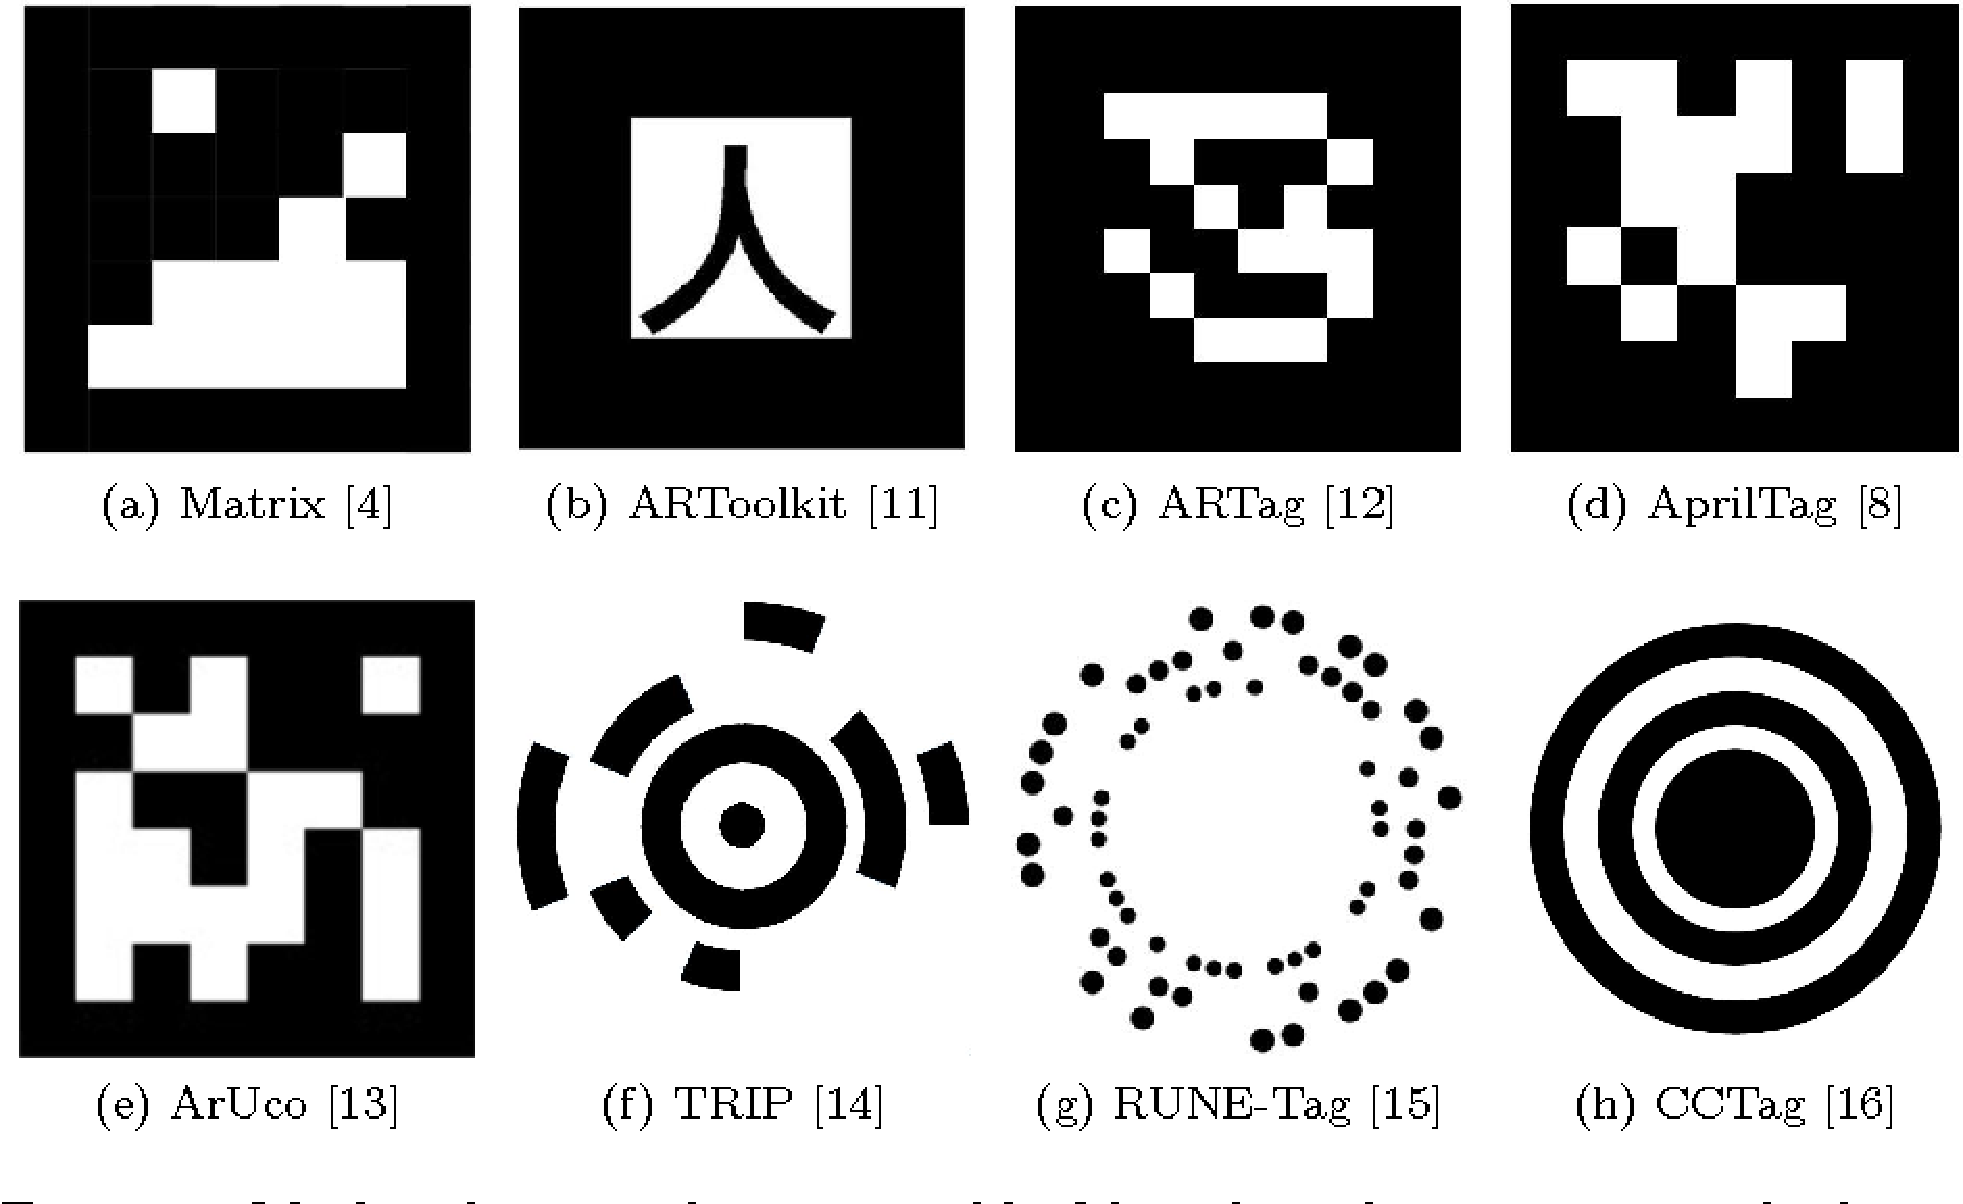
\includegraphics[width = 0.9\textwidth, trim={0 12mm 0 0}, clip]{immagini/esempio-markers.pdf}
	\caption{Esempio di marcatori fiduciali.}
	\label{fig:esempio_markers}
\end{figure}
\\
La tesi è strutturata nel seguente modo:
\begin{itemize}
	\item Capitolo \ref{chap:analisi_problema}: Analisi del problema\\
	Presenta un'analisi del problema da risolvere e la spiegazione ad alto livello della soluzione proposta.
	
	\item Capitolo \ref{chap:archi_sistema}: Architettura del sistema\\
	In questo capitolo viene affrontato in maniera dettagliata la struttura di tutto il sistema e delle varie scelte che sono state affrontate.
	
	\item Capitolo \ref{chap:prove_sperimentali}: Prove sperimentali\\
	Questa parte è dedicata ai test fatti sul simulatore e su un drone reale. Viene spiegato l'ambiente in cui i test vengono effettuati, la configurazione del drone e un'analisi dei risultati ottenuti.
	
	\item Capitolo \ref{chap:conclusione_sviluppi_futuri}: Conclusione e sviluppi futuri\\
	Infine nell'ultimo capitolo è presente una valutazione dei risultati ottenuti rispetto all'obiettivo prefissato; inoltre sono presenti delle proposte di miglioramento del sistema per eventuali sviluppi futuri.
\end{itemize}


%   CAPITOLO 2: 
\chapter{Analisi del problema}
\label{chap:analisi_problema}

\section{Obiettivo}
\label{sec:problema:obiettivo}
L'obiettivo di questa tesi è quello di studiare, progettare e realizzare un sistema autonomo in grado di eseguire una missione precedentemente impostata, utilizzando come sistema di navigazione la VO, nello scopo di analizzare dei marker noti e fissi. Il sistema è pensato per essere utilizzato in un ambiente chiuso, ad esempio un magazzino; di conseguenza, i marker dovrebbero essere posizionati sul soffitto, in modo tale da minimizzare la probabilità di non vederli; ma, per questioni di praticità, i marker vengono fissati al pavimento. \\
Gli obiettivi principali sono due:
\begin{itemize}
	\item Creare un sistema che cattura le immagini dalla camera, le analizza trovandone i marker e la loro posizione relativa all'ambiente e infine invia questi dati al flight controller.
	\item Sviluppare un programma che permetta di eseguire delle missioni precedentemente programmate e completamente personalizzabili. Le missioni saranno composte da una lista di obiettivi (target) e deve essere possibile impostare due modalità di target: la prima, in cui l'UAV arriva al punto scelto, si ferma fino a posizionarsi correttamente nel punto desiderato e poi continua la missione raggiungendo il punto successivo (hoverpoint); nella seconda modalità il drone arriva al target e passa direttamente al prossimo, senza fermarsi (waypoint).
\end{itemize}

\section{Soluzioni proposte in letteratura}
In letteratura sono presenti diverse strategie per risolvere il problema della localizzazione senza utilizzare la geolocalizzazione. Esse si dividono in due categorie: map-based e mapless \cite{CHANG2023104533}.
\begin{itemize}
	\item Map-based: a sua volta si dividono in due categorie: Known Map e Map-building.\\
	Nel primo caso, il sistema contiene delle informazioni sull'ambiente. Alcuni esempi sono la VO basata sui marker e l'utilizzo di radiofrequenze, dove attraverso l'analisi della Radio Signal Strength Indicator (RSSI) è possibile calcolare la distanza tra trasmettitore e ricevitore. In entrambi questi esempi è necessario che il drone sappia dove siano i marker/antenne per stimale la propria posizione. \\
	Nel secondo caso il sistema deve costruirsi internamente una mappa locale/globale dell'ambiente, mentre lo esplora. Questa tecnica viene chiamata Simultaneous Localization and Mapping (SLAM). Due esempi sono V-SLAM (sfrutta le immagini) e Lidar-SLAM (il lidar permette di calcolare il time-of-flight tra il sensore e l'ostacolo, di conseguenza la posizione).
	\item Mapless: esistono tre approcci: integrato, diretto e indiretto. nel primo approccio le informazioni dei sensori vengono direttamente trasformate in comandi per il drone, senza un'unità di controllo intermedia. L'approccio diretto estrae dalle immagini informazioni sull'ambiente e le invia a un'unità di controllo separata; quest'ultima ne determina i comandi di navigazione. Infine, l'approccio indiretto stima le distanze dagli ostacoli e fornisce queste informazioni a un'unità di controllo, che decide come modificare la traiettoria per evitare collisioni.
\end{itemize}
Per risolvere il nostro obiettivo la conoscenza della mappa è fondamentale, quindi le ricerce sono state concentrate in questa direzione.
\\ \\
A questo punto, i due approcci che possiamo confrontare sono Known Map e Map-building. Questo articolo \cite{7955787} confronta VO e SLAM, arrivando alla conclusione che la VO è l'approccio migliore perché risulta più veloce e richiede memoria e risorse computazionali inferiori rispetto a SLAM.
\\ \\
In questo articolo \cite{s22155798} propongono un UAV multirotore dove viene usata la VO basata sui marker come strumento di localizzazione. Il sistema proposto è pensato per la navigazione in ambienti al chiuso. Il sistema utilizza la seconda versione del Robot Operating System (ROS 2) \footnote{\url{https://www.ros.org/}} come libreria software per l'implementazione della VO; inoltre è stato scelto AprilTag come marker fiduciale. Un'altro articolo \cite{6549921} propone un sistema che sfrutta ROS per processare i dati arrivati dalla camera, mentre come marker propone l'utilizzo di ARTag. \\
In conclusione entrambi sistemi, anche se utilizzano architetture differenti, hanno dimostrato risultati più che sufficienti.
\\ \\
Un'altro approccio sempre basato sulla VO, ma senza l'utilizzo dei marker, è stato proposto in quest articolo \cite{4752770}. In molti edifici sono presenti dei soffitti con delle figure regolari, ad esempio un mosaico di quadrati. Il loro sistema consiste nel sfruttare queste figure per stimare posizione e posa del sistema, confrontando frame per frame l'immagine precedente con la successiva, e quindi stimando in che direzione il sistema si è spostato.
\\ \\
Tutte le architetture proposte in letteratura utilizzano il filtro di Kalman, un algoritmo matematico che restituisce un'ottima stima di posizione e posa del modello \cite{CHANG2023104533} \cite{7955787} \cite{8483685} \cite{s22155798} \cite{s19245480}. L'argomento viene approfondito nel paragrafo \ref{sec:problema:localizzazione:kalman}. 

\section{L’approccio proposto}
Analizzando gli obiettivi e i metodi proposti in letteratura, la soluzione proposta prevede l'utilizzo di un UAV dotato dei classici sistemi per il volo autonomo ad escluzione del ricevitore GPS, dato che non verrà utilizzato.  \\
Uno degli obiettivi è quello di creare un sistema che sfrutti la VO tramite marker per la localizzazione; di conseguenza è necessario installare sul drone con companion computer dotato di camera. È stato scelto un Raspberry Pi 3 con una camera OV7251 global shutter rivolta verso il basso, in modo tale che il sistema possa visualizzare il pavimento per poter localizzare i marker. Il Raspberry Pi 3, oltre ad eseguire il programma per la VO, deve ospitare il sistema per la gestione della missione. Entrambi i programmi sono scritti in Python, per questioni di praticità e sicurezza.\\
Tutte le comunicazioni tra il companion computer e il flight controller del drone vengono effettuate attraverso il protocollo MAVLink, sfruttando il GPIO (General Purpose Input/Output, una interfaccia hardware) del Raspberry e l'interfaccia seriale del flight controller Holybro Pixhawk 6C Mini. \\
Nelle sezioni \ref{sec:problema:localizzazione} e \ref{sec:problema:missione} vengono spiegate in modo più approfondito l'approccio adottato per la localizzazione e la missione.

\section{Sistema di localizzazione}
\label{sec:problema:localizzazione}
Come precedentemente spiegato, il sistema di localizzazione usa dei marker come punto di riferimento e, dopo l'elaborazione da parte del companion computer, i risultati saranno inviati al flight controller che li elaborerà per stimare posizione e posa. \\
In questo paragrafo vengono approfonditi questi due passaggi: la scelta del marker e come viene stimato lo stato interno dentro al flight controller.
\subsection{Marker}
In questo articolo \cite{fiducialMarker2021} viene svolta un'analisi di varie tipologie di marker usati nel campo della robotica. Quelli che vengono analizzati in modo più approfondito sono ARTag, AprilTag, ArUco e STag, ovvero quelli maggiormente utilizzati per l'obiettivo richiesto. \\ L'esperimento consiste nel testare ogni marker in condizioni di luce, posizione e orientamento, numero di marker visibili contemporaneamente e costo computazionale in base all'hardware scelto diversi. \\
Le conclusioni dell'esperimento mostrano che il marker ArUco presenta la miglior soluzione: ha presentato ottimi risultati nel calcolo della posizione e posa; un'ottima velocità di rilevamento; un buon costo computazionale e il migliore in termini di memoria utilizzata. D'altra parte, è molto sensibile in caso il marker sia molto piccolo oppure sia distante; infine il costo computazionale scala in base al numero di marker presenti dell'immagine. Il primo problema lo possiamo escludere dato che l'ambiente per cui il sistema è stato pensato è un posto chiuso, quindi la distanza massima del drone dal marker dipende dall'altezza dell'ambiente; il secondo problema non si può completamente risolvere, ma si può ridurre facendo un'analisi e scegliendo la posizione di ogni marker in base all'ambiente e alla missione che si dovrà eseguire, con l'obiettivo che la camera del drone visualizzi almeno un marker fino ad un massimo di quattro (perché vogliamo vederne almeno due, quindi nel caso peggione ne vediamo quattro). In Fig. \ref{fig:esempio_aruco} sono presenti un esempio di marker ArUco.
\begin{figure}
	\centering
	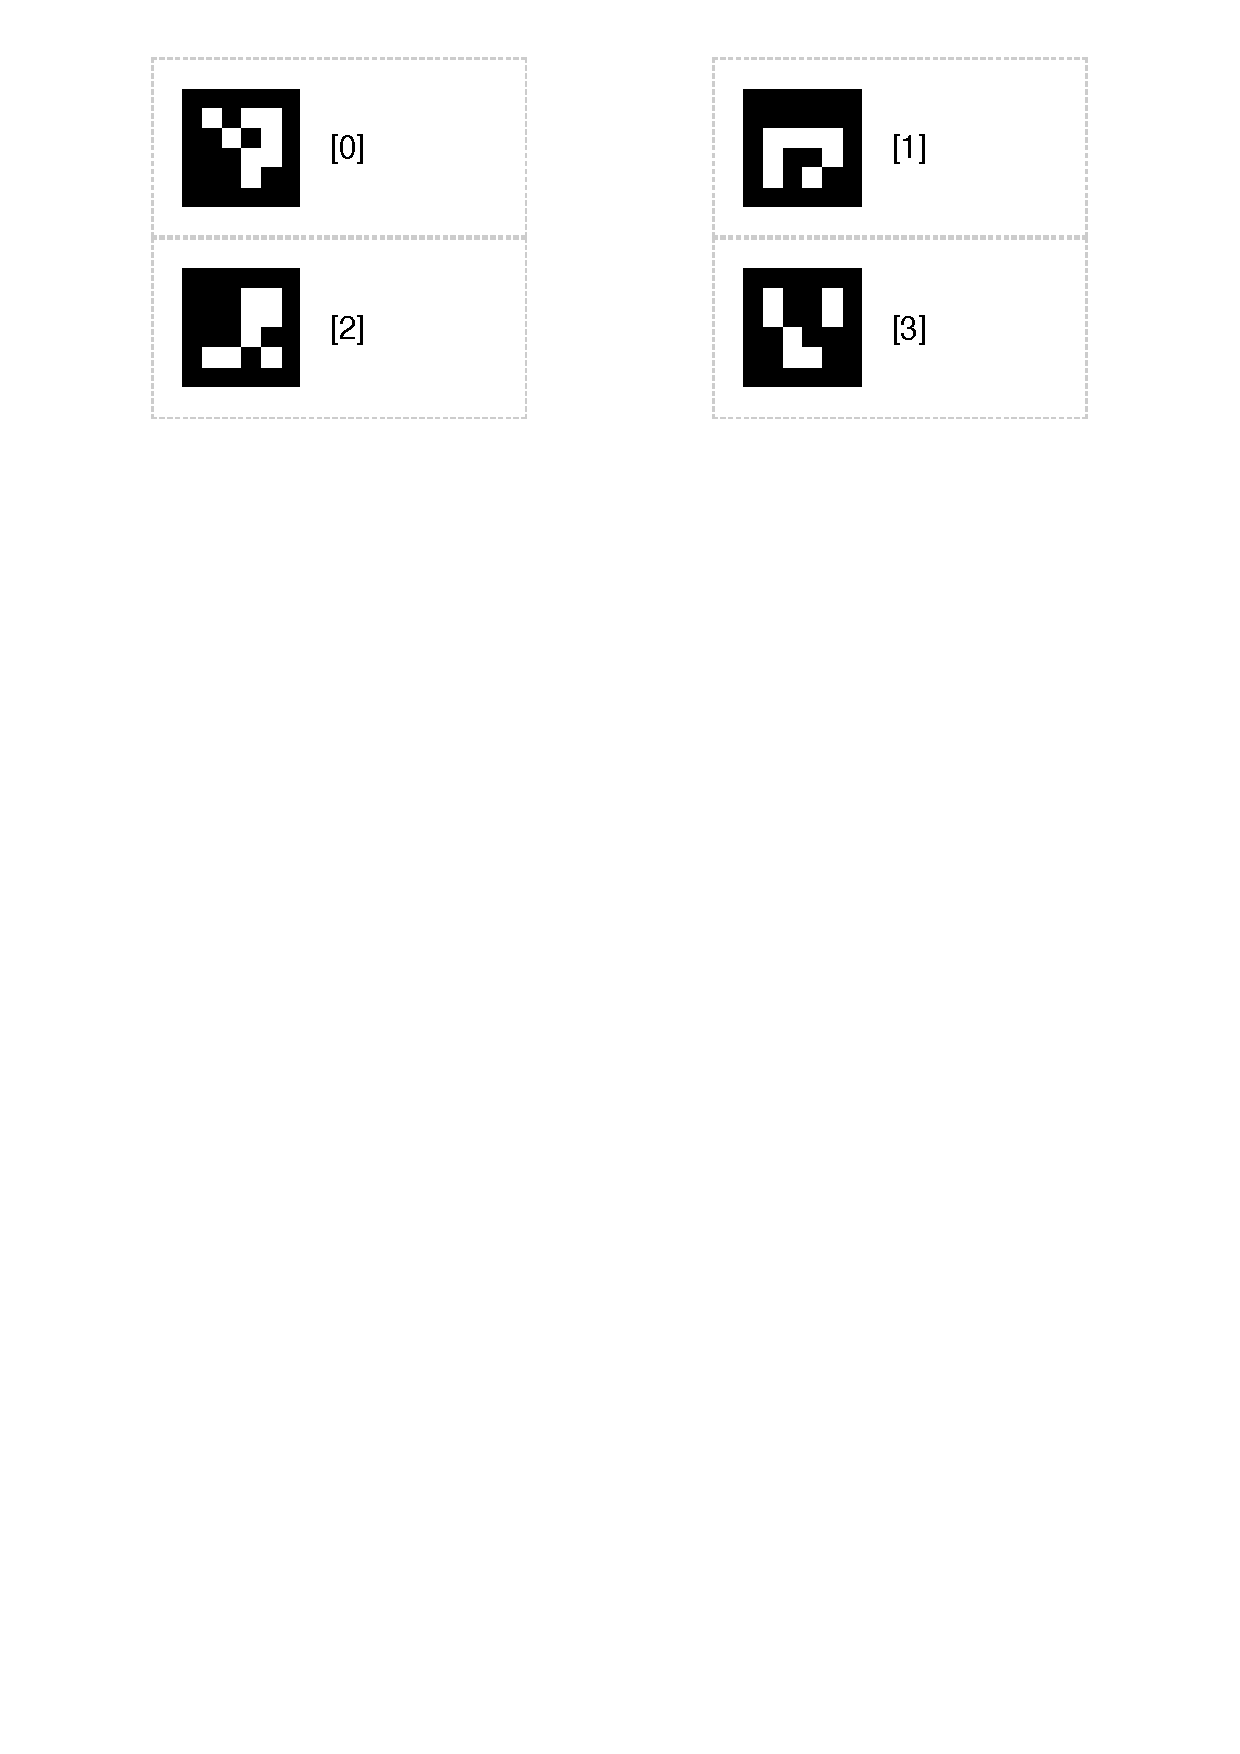
\includegraphics[width = 0.9\textwidth, trim={0 0 0 0}, clip]{immagini/esempio-aruco.pdf}
	\caption{Esempio di quattro marker ArUco 4x4 col il relativo ID.}
	\label{fig:esempio_aruco}
\end{figure}
\subsection{Filtro di Kalman}
\label{sec:problema:localizzazione:kalman}
Analizzando il sistema, possiamo pensare che solamente la VO ci dia le informazioni di posizione e posa dell'UAV; in realtà, dentro al flight controller esiste un'altro componente che direttamente o indirettamente può darci le stesse informazioni, ovvero l'IMU (Inertial Measurement Unit). Questo dispositivo contiene all'interno vari componenti: accellerometro, giroscopio e opzionalmente un magnetometro; a noi interessano i primi due: il primo ci permette di stimare la posizione del drone rispetto alle sue coordinate di partenza, sfruttando la lettura delle accellerazioni subite; mentre il secondo dispositivo ci fornisce le informazioni di posa. Tuttavia l'IMU ha un grosso problema, ovvero che l'errore di stima della posizione aumenta con il passare del tempo; questo è dovuto dal fatto che il sensore, anche se calibrato correttamente, presenta un'incertezza che si propaga nel tempo (drift); di conseguenza, quando viene calcolata la doppia integrazione per passare dall'accellerazione alla posizione, l'errore diventa esponenziale. \\
Questo non vuol dire che dobbiamo buttare le informazioni dell'IMU; possiamo fonderle ai dati che ci arrivano da altri sensori più affidabili, ad esempio dal GNSS o dalla VO. Questo è possibile attraverso un algoritmo matematico ricorsivo chiamato filtro di Kalman; esso permette di stimare lo stato interno di un sistema dinamico a partire da una sequenza di misurazioni che presentano rumore e incertezza. In particolare, nei droni viene usata una sua variante chiamata Extended Kalman Filter (EKF), che permette di gestire sistemi non lineari.
\\
\begin{figure}
	\centering
	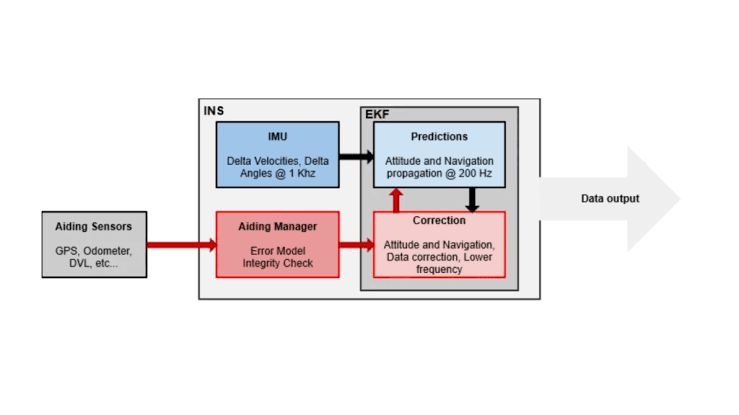
\includegraphics[width = 1\textwidth, trim={0 0 0 0}, clip]{immagini/filtro-kalman.png}
	\caption{Principio base del funzionamento di un Extended Kalman Filter (EKF).}
	\label{fig:esempio_ekf}
\end{figure}
\\
L'EKF utilizzato nel PX4 Autopilot è la versione due, chiamato EKF2\footnote{\url{https://docs.px4.io/main/en/advanced_config/tuning_the_ecl_ekf}} \footnote{\url{https://www.youtube.com/watch?v=CMGQJNPiTJg&t=39s}}.

\section{Struttura della missione}
\label{sec:problema:missione}
La missione viene descritta attraverso un file json e contiene una lista di target da raggiungere. Ogni obiettivo ha vari parametri, alcuni opzionali e alcuni no:
\begin{itemize}
	\item {\em north\_m, east\_m, down\_m} (obbligatori): indicano le coordinate NED della posizione dell'obiettivo che si vuole raggiungere, rispetto al sistema di riferimento locale. La posizione è espressa in metri.
	\item {\em yaw\_deg} (opzionale): esprime l'angolo yaw desiderato in gradi. Il valore di default è 0.
	\item {\em hover\_time\_ms} (opzionale): indica il tempo di attesa del drone, dopo aver correttamente raggiunto l'obiettivo corrente, prima di passare al prossimo obiettivo. Viene espresso in millisecondi. Il valore di default è 0.
	\item {\em vel\_m\_s} (opzionale): esprime la velocità che l'UAV avrà fino al raggiungimento del target o in prossimità di esso, espressa in metri al secondo. Il suo valore di default è null, e rappresenta l'assenza di impostare una velocità fissa.
	\item {\em expiration\_time\_s} (opzionale): indica il tempo dopo il quale il target in corso scade. La velocità del drone viene impostata in modo tale che l'UAV possa raggiungere il target nel tempo prestabilito. È espresso in secondi. Il suo valore di default è null, e rappresenta l'assenza del tempo di scadenza del target.
\end{itemize}
Le due modalità di target che sono fissate come obiettivi sono hoverpoint e waypoint. Un metodo per eseguire la prima modalità è senza impostare i valori {\em vel\_m\_s} o {\em expiration\_time\_s}; in questo modo, l'UAV prima di passare al prossimo obiettivo deve raggiungere correttamente quello corrente. Invece usando uno di questi parametri è possibile impostare il target in modalità waypoint.

%   CAPITOLO 3: 
\chapter{Architettura del sistema}
\label{chap:archi_sistema}
In questo capitolo viene descritto in modo più approfondito il sistema del drone reale e il suo funzionamento.

\section{Struttura generale del sistema}
\subsection{Flight controller}
Per la realizzazione del sistema è stato scelto Holybro Pixhawk 6C Mini\footnote{\url{https://docs.px4.io/main/en/flight_controller/pixhawk6c_mini}}, un flight controller compatibile con il firmware PX4 Autopilot. La scelta è stata dettata dalla possibilità di sfruttare le stesse funzionalità di stima dello stato e di controllo del volo imlementate nel firmware, nonché le stesse presenti sul simulatore. Inoltre, le interfacce integrate consentono di creare un canale di comunicazione diretto tra esso e il companion computer.
\subsection{Companion computer}
Il companion computer deve essere un'unità in grado di poter elaborare le immagini, eseguire la missione e allo stesso tempo deve avere un consumo moderato, temperature gestibili e dimensioni ridotte; per questo è stato scelto un Raspberry Pi 3B\footnote{\url{https://www.raspberrypi.com/products/raspberry-pi-3-model-b/}}, un computer di piccole dimensioni compatibile con Linux, quindi in grado di eseguire gli stessi script usati nel simulatore; una cpu con architettura ARM, che permette di avere consumi e temperature ridotte; modulo Wi-Fi, permette di potersi collegare al terminale della scheda senza cavi; GPIO e Camera Serial Interface (CSI), per potersi connettere al flight controller attraverso la porta seriale e poter installare una camera. \\
Il Raspberry ha installato una camera global shutter OV7251 (Sec. \ref{sec:vo:camera} per ulteriori dettagli). \\
Infine, la scheda viene alimentata attraverso un modulo step-down adeguato, che abbassa la tensione da \qty{14.8}{\volt} della batteria del drone ai \qty{5}{\volt} necessari al Raspberry. Prestare molta attenzione nella scelta di questo componente, perché un'opzione errata potrebbe bruciare la scheda.
\subsection{QGroundControl}
La configurazione e il monitoraggio del drone sono affidati al software QGroundControl\footnote{\url{https://qgroundcontrol.com/}}. Esso permette di interagire con il firmware PX4 Autopilot attraverso il protocollo MAVLink\footnote{\url{https://mavlink.io/en/}}, un sistema di comunicazione di tipo publish-subscribe e punto-punto molto leggero usato in ambito droni. \\
Questo software è stato utilizzato per configurare i parametri del flight controller, verificare lo stato del drone, scaricare i log generati e infine controllare il drone (armarlo, muoverlo attraverso i joistick, cambiare modalità, \ldots).

\section{Architettura software del sistema}
Per mantenere separate le responsabilità delle varie componenti, il software è stato organizzato creando due classi principali; una per l'elaborazione visiva (\texttt{VisualOdometry}) e l'altra (\texttt{DroneMavlink}) per gestire comunicazione e missione tra il companion computer e il flight controller. In questo modo il codice risulta più modulare e rende più semplice lo sviluppo e la manutenzione. \\
Nei seguenti paragrafi vengono presentati la struttura e i vari collegamenti di tutti i sistemi; inoltre, vengono presentate in modo più approfondito le soluzioni agli obiettivi descritti nel paragrafo \ref{sec:problema:obiettivo}. \\ \\
È possibile visualizzare tutti gli script creati e la struttura del sistema su github\footnote{\url{https://github.com/filipporaciti/px4-mark-position}}.

\subsection{Struttura generale: i moduli funzionali}
Nella Fig. \ref{fig:schema_software} è possibile visualizzare lo schema generale del software. I componenti principali sono le due classi \texttt{VisualOdometry} e \texttt{DroneMavlink}, che si occupano rispettivamente dell'elaborazione delle immagini e della comunicazione con il flight controller. \\
L'esecuzione della VO viene affidata al file \texttt{send\_position.py}, che si occupa dell'aquisizione del frame dalla camera; successivamente l'immagine viene elaborata dalla classe \texttt{VisualOdometry}, che si occupa del rilevamento dei marker e del calcolo della posizione e posa del drone. Le informazioni ottenute verranno poi inviate grazie alla classe \texttt{DroneMavlink} al flight controller, utilizzando il protocollo MAVLink.\\
La gestione della missione viene invece affidata al file \texttt{mission.py}. Esso si occupa di recuperare la missione ed eseguirla, richiamando la funzione presente nella classe \texttt{DroneMavlink}.\\
Infine, il file \texttt{position\_mission.py} si occupa di eseguire insieme tutti i sistemi descritti precedentemente, in modo da evitare conflitti di concorrenza nell'utilizzare il protocollo MAVLink sullo stesso canale seriale.

\begin{figure}[!htbp]
	\centering
	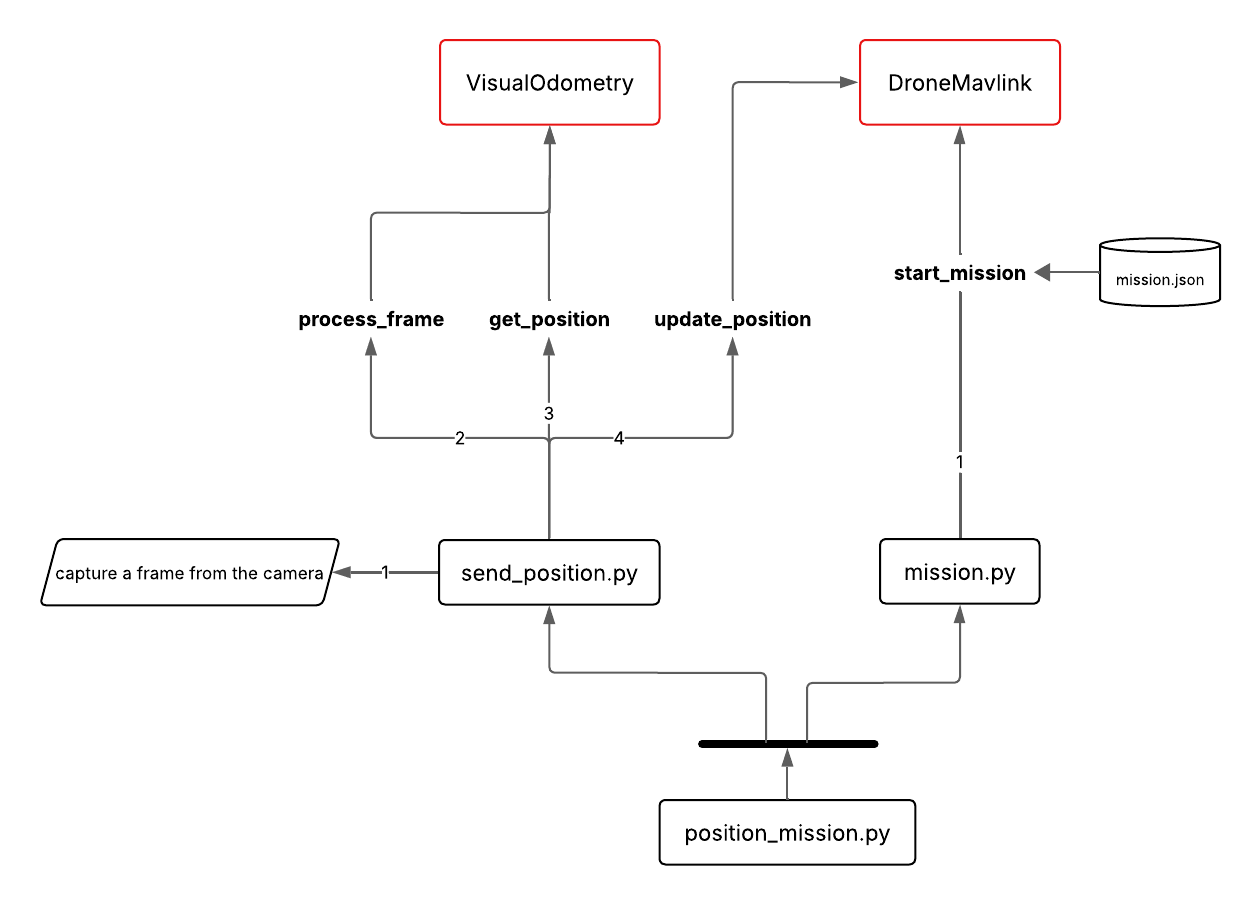
\includegraphics[width=1\textwidth, trim={0 0 0 0}, clip]{immagini/schema_software.png}
	\caption{Schema dell'architettura software e visualizzazione del flusso delle informazioni tra i moduli del sistema.}
	\label{fig:schema_software}
\end{figure}

\section{Mission}
La gestione della missione è stata imlementata utilizzando la modalità Offboard di PX4\footnote{\url{https://docs.px4.io/main/en/flight_modes/offboard}}, controllata attraverso il protocollo MAVLink. A differenza delle missioni gestite direttamente dal controllore di volo attraverso QGroundControl, questa soluzione permette di avere maggiore libertà e controllo sul volo.\\
La missione è composta da una lista ordinata di target, ciascuno con le proprie caratteristiche. Il software si occupa di gesitre le diverse fasi della missione, dall'avvio fino al completamento, verificando il raggiungimento dei target e gestendo il passaggio da un punto all'altro.\\ \\

\subsection{Architettura}
La missione viene eseguita interamente dalla classe \texttt{DroneMavlink}. All'interno essa utilizza il modulo \texttt{mavsdk}\footnote{\url{http://mavsdk-python-docs.s3-website.eu-central-1.amazonaws.com/}}, un insieme di librerie che permettono di comunicare con i sistemi che utilizzano il protocollo MAVLink. \\
La classe \texttt{DroneMavlink} contiene una funzione chiamata \texttt{start\_mission} che richiede solamente un parametro, la missione da eseguire. Essa viene rappresentata da un dizionario contenente la lista di target (esempio nella Lst. \ref{lst:esempio_missione}).
\begin{lstlisting}[language=json, caption={Esempio di configurazione della missione}, label={lst:esempio_missione}]
	{
		"targets": [
			{
				"north_m": 0.0,
				"east_m": 0.0,
				"down_m": -1.5
			},
			{
				"north_m": 3.0,
				"east_m": 3.0,
				"down_m": -1.5,
				"hover_time_ms": 1000
			}
		]
	}
\end{lstlisting}
Il compito di \texttt{start\_mission} è quello di gestire tutte le fasi principali della missione. In ordine, si occupa di inizializzare il collegamento con il flight controller; fa dei controlli pre-volo e attende finchè il sistema non ha tutti i requisiti per decollare; avvia la modalità Offboard di PX4; fa decollare il drone, impostando come target il parametro \texttt{TAKEOFF\_TARGET} della classe \texttt{DroneMavlink}, ovvero un obiettivo predefinito che indica la posizione che il drone deve raggiungere per il decollo; successivamente vengono iterati e impostati come obiettivo tutti i target, uno ad uno; infine viene cambiata la modalità del drone da Offboard a Land, che permette di far atterrare il drone e di disarmarlo in automatico. \\
Non è stata utilizzata la modalità Takeoff di PX4 perché, con la soluzione implementata in questo sistema, è possibile sfruttate tutti i vantaggi di personalizzazione dei target. \\ \\
Nella sezione \ref{sec:archi:target} viene descritto come singolarmente il drone raggiunge ogni target; in particolare, viene spiegato come sono state implementate tutte le opzioni presentate nella Sez. \ref{sec:problema:missione}.

\subsection{Target}
\label{sec:archi:target}
La funzione che permette di raggiungere un target si chiama \texttt{move\_to}, e riceve come parametro una \texttt{NamedTuple} chiamata \texttt{Target}. La lista degli elementi, con i vari valori di default, è presente della Lst. \ref{lst:target}.
\begin{lstlisting}[style=pythonstyle, caption={Lista degli elementi che un Target ha}, label={lst:target}]
class Target(NamedTuple):
	north_m: float
	east_m: float
	down_m: float
	yaw_deg: float = 0.0
	hover_time_ms: int = 0
	expiration_time_s: float = None
	vel_m_s: float = None
\end{lstlisting}
Non è necessario approfondire singolarmente ogni campo della struttura. Quelli che meritano una maggiore attenzione sono come le modalità hoverpoint e waypoint del target vengono attivate e il loro funzionamento.
\subsubsection{Hoverpoint}
Questa modalità permette al drone di raggiungere il target e di attendere il suo stazionamento. La posizione desiderata viene definita dalle tre coordinate \texttt{north\_m}, \texttt{east\_m} e \texttt{down\_m}, espresse nel sistema di riferimento NED (Sez. \ref{sez:archi:vo:pos}).\\ \\
Nella Fig. \ref{fig:diag_flusso_hoverpoint} è presente lo schema che descrive il funzionamento base di questa modalità. La prima istruzione che viene inviata al drone è quella di raggiungere un certo obiettivo; questo viene fatto attraverso la funzione \texttt{set\_position\_ned}. Successivamente, vengono monitorate in sequenza posizione, velocità e yaw per vedere quando il drone converge verso il suo obiettivo, seguendo le tolleranze impostate nella classe \texttt{DroneMavlink}.
\begin{figure}[!htbp]
	\centering
	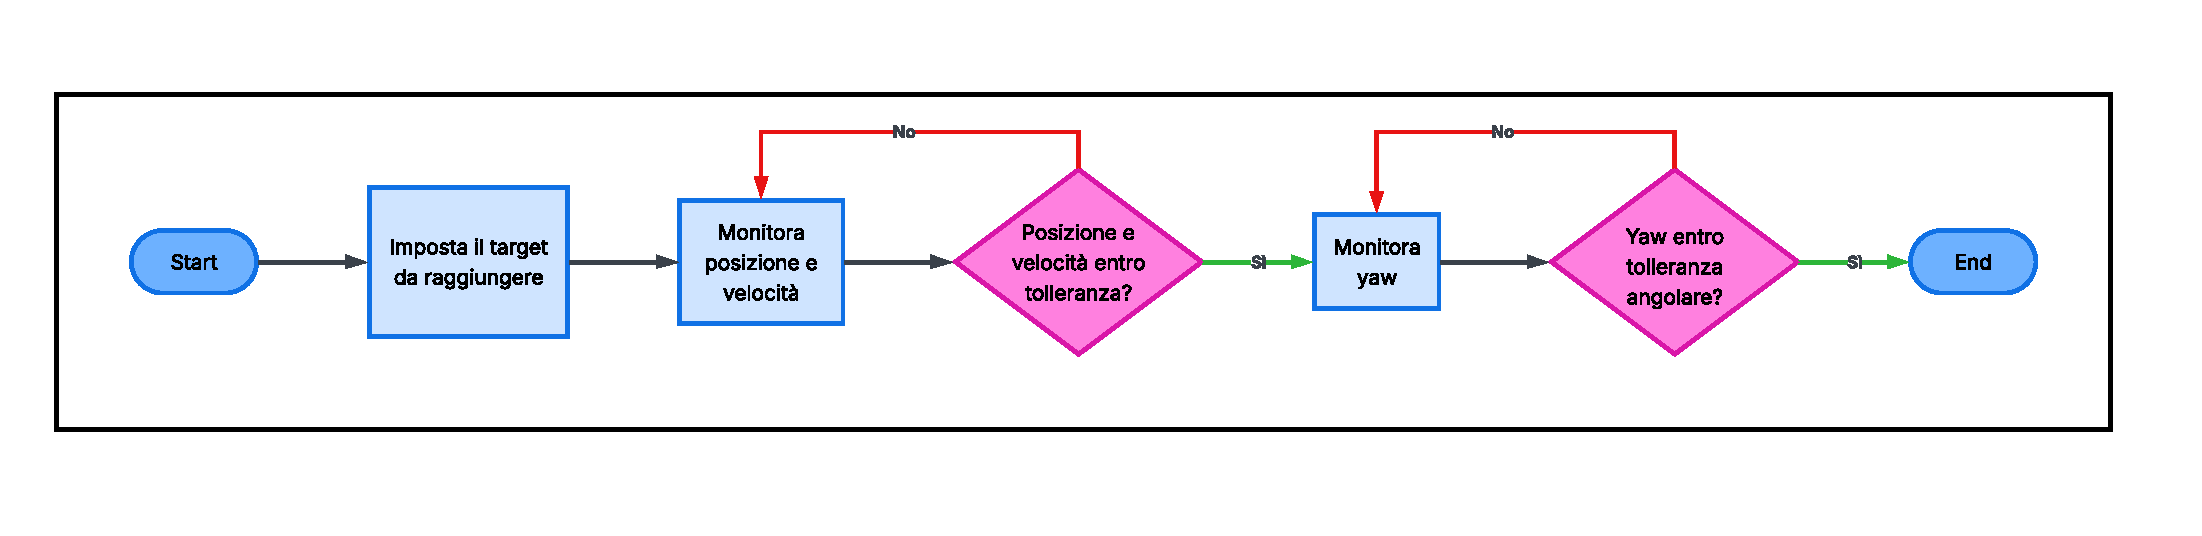
\includegraphics[width=0.95\textwidth, trim={0 0 0 0}, clip]{immagini/diagramma_flusso_hoverpoint.pdf}
	\caption{Diagramma di flusso della modalità hoverpoint di un target.}
	\label{fig:diag_flusso_hoverpoint}
\end{figure}

\subsubsection{Waypoint}
La modalità waypoint consente di raggiungere un obiettivo senza doversi fermare. È possibile creare un target che esegui questa modalità impostando uno dei due parametri \texttt{expiration\_time\_s} o \texttt{vel\_m\_s}. Essi indicano direttamente la velocità NED di dove il drone deve andare (usando alla funzione \texttt{set\_velocity\_ned}) e per quanto tempo mantenerla.  \\ \\
Nella Fig. \ref{fig:diag_flusso_waypoint} è rappresentato un diagramma di flusso del funzionamento base della modalità waypoint. Le parti che meritano un approfondimento sono due: il secondo blocco di decisione, dove vengono separati i vari calcoli delle velocità nei casi in cui si utilizza \texttt{expiration\_time\_s} da quello di \texttt{vel\_m\_s}; e l'ultimo blocco istruzione, dove viene dato il comando di impostare le coordinate NED della posizione.

\begin{figure}[!htbp]
	\centering
	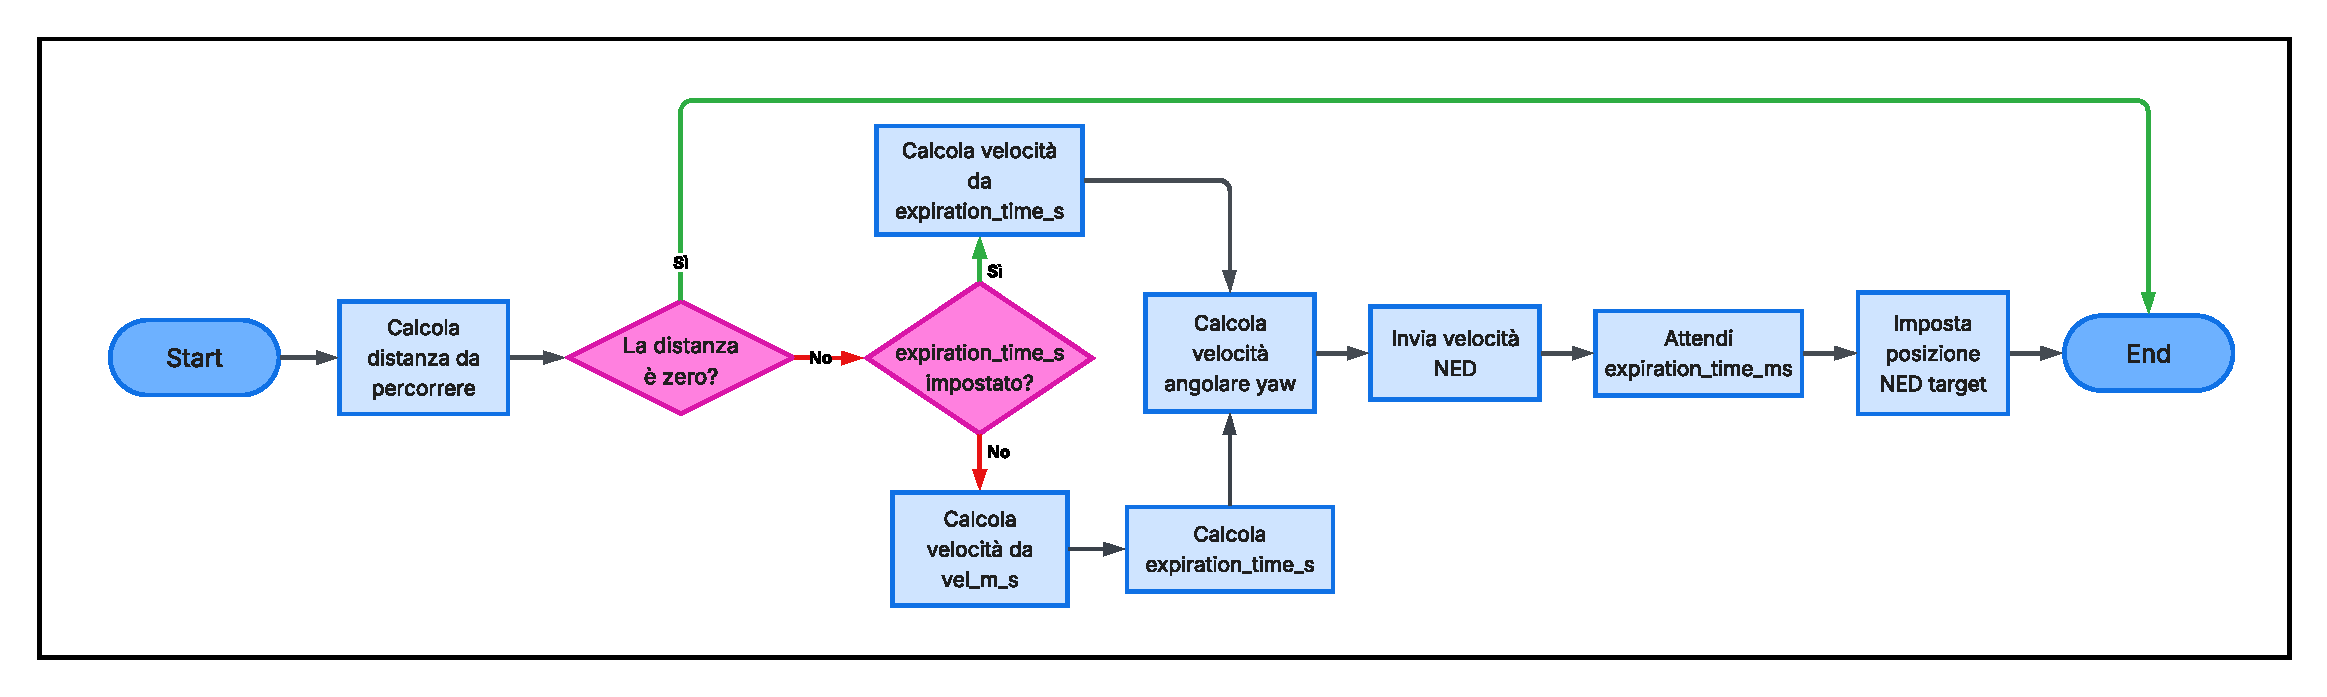
\includegraphics[width=1\textwidth, trim={0 0 0 0}, clip]{immagini/diagramma_flusso_waypoint.pdf}
	\caption{Diagramma di flusso della modalità waypoint di un target.}
	\label{fig:diag_flusso_waypoint}
\end{figure}

\paragraph{expiration\_time\_s} Avendo impostato il tempo che il drone ci mette per raggiungere il suo obiettivo ($t_\mathrm{exp\_time}$), la velocità per ogni coordinata si può calcolare in modo molto semplice facendo:
\[
\begin{bmatrix}
	v_N \\
	v_E \\
	v_D
\end{bmatrix}
=
\frac{1}{t_\mathrm{exp\_time}}
\cdot
\begin{bmatrix}
	\Delta N \\
	\Delta E \\
	\Delta D
\end{bmatrix}
\]

\paragraph{vel\_m\_s} Per calcolare la velocità NED partendo dalla velocità di crociera desiderata ($v_\mathrm{target}$), bisogna inanzitutto calcolare la distanza:
\[
d =
\sqrt{
	\Delta N^2 +
	\Delta E^2 +
	\Delta D^2
}
\]
Definiamo il vettore $\Delta p$, che indica la distanza tra il vecchio e il nuovo target:
\[
\Delta p =
\begin{bmatrix}
	\Delta N \\
	\Delta E \\
	\Delta D
\end{bmatrix}
\]
Non possiamo assegnare direttamente $v_\mathrm{target}$ in modo uguale per ogni coordinata. Quindi, dobbiamo distribuirla in modo proporzionale allo spostamento. Per fare ciò, dividiamo il vettore $\Delta p$ per la distanza calcolata precedentemente:
\[
\hat{u} =
\frac{\Delta p}{d}
\]
Successivamente, la velocità NED si può calcolare in questo modo:
\[
\begin{bmatrix}
	v_N \\
	v_E \\
	v_D
\end{bmatrix}
=
v_\mathrm{target}\cdot \hat{u}
\]
L'altro parametro necessario per il sistema è $t_\mathrm{exp\_time}$:
\[
t_\mathrm{exp\_time} = \frac{d}{v_\mathrm{target}}
\]

\paragraph{Comando posizione finale} Per concludere, il comando \texttt{set\_velocity\_ned} imposta la velocità nelle varie coordinate NED del drone, senza mai fermarsi. È per questo che viene inviato il comando \texttt{set\_position\_ned} alla fine del blocco di codice, per evitare problematiche di questo tipo. Un possibile problema reale lo si potrebbe riscontrare nel caso in cui l'ultimo target della missione è un target di questo tipo, quindi il drone inizia la manovra di atterraggio e potrebbe cadere, dato che atterra mentre è in movimento; oppure nel caso in cui viene impostato anche il parametro \texttt{hover\_time\_ms} (un utilizzo insolito, ma comunque possibile).

\section{Visual odometry}
L'architettura della VO si può dividere in due parti: software e hardware. In questa sezione vengono affrontati entrambi gli aspetti, approfondendo principalmente l'architettura nel drone reale.

\subsection{Cattura e analisi del frame}
È stato scelto il modulo Python \texttt{picamera2}\footnote{\url{https://pip-assets.raspberrypi.com/categories/652-raspberry-pi-camera-module-2/documents/RP-008156-DS-7-picamera2-manual.pdf}} per l'acquisizione dei frame dalla camera. Nella Sez. \ref{sec:vo:camera} viene approfondita la configurazione dei vari parametri della camera. In particolare, viene utilizzata la funzione \texttt{picamera2.capture\_request} in modalità asincrona, impostando il parametro \texttt{signal\_function}; in questo modo, quando il frame è disponibile, verrà automaticamente richiamata la funzione impostata nel parametro \texttt{signal\_function}, che si occuperà di elaborare il frame e inviare i dati al flight controller. \\
Un diagramma di flusso che rappresenta l'implementazione di questa funzione è presente nella Fig. \ref{fig:diag_flusso_frame_an}. 
\begin{figure}[!htbp]
	\centering
	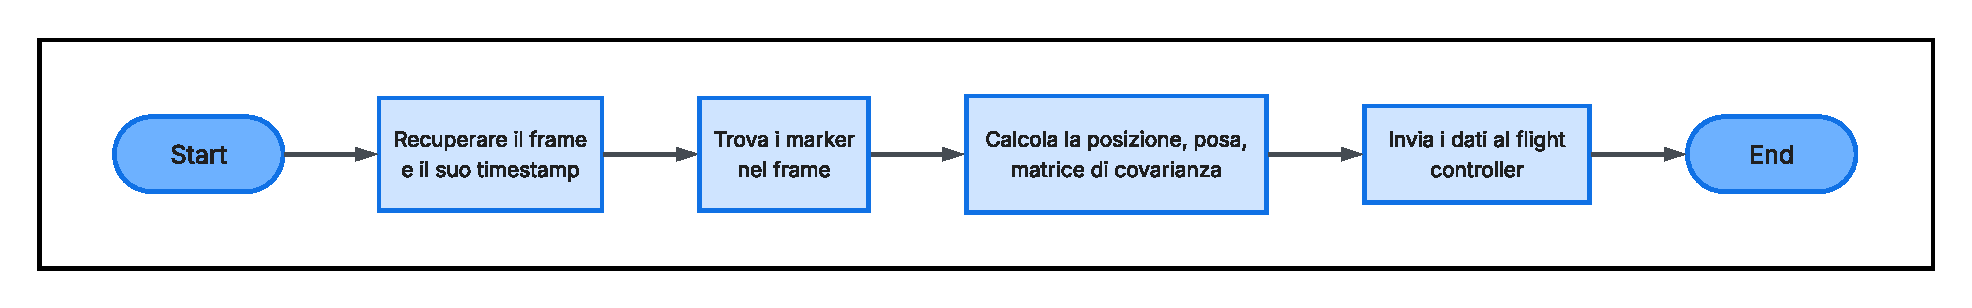
\includegraphics[width=1\textwidth, trim={0 0 0 0}, clip]{immagini/diagramma_flusso_frame_analyzer.pdf}
	\caption{Diagramma di flusso della funzione richiamata dal modulo \texttt{picamera2} per l'analisi del frame.}
	\label{fig:diag_flusso_frame_an}
\end{figure} \\
Prima di approfondire i calcoli di posizione, posa e della matrice di covarianza bisogna fare una considerazione sui marker, ovvero stabilire che azione intraprendere in caso l'immagine contenga più di un marker. Le principali opzioni disponibili sono tre: analizzare tutti i marker presenti, analizzarne alcuni, oppure analizzarne uno in particolare. \\
È stata scelta l'ultima opzione, perchè consente di effettuare la VO mantenendo una frequenza di calcolo abbastanza costante. I marker candidati vengono ordinati secondo la grandezza della propria superficie, in ordine decrescente. Il calcolo dell'area dei marker è stata eseguita utilizzando la formula dell'area di Gauss (chiamata anche Shoelace Formula o Green’s Formula)\footnote{\url{https://www.baeldung.com/cs/2d-polygon-area}}. \\
Infine, è stata aggiunta la possibilità di avere marker con dimensione diversa nello stesso ambiente. Questo consente di risolvere alcuni problemi di visibilità della camera o di aumentare la precisione del volo in alcune zone prestabilite.

\subsection{Calcolo della posizione}
\label{sez:archi:vo:pos}
Durante lo sviluppo del sistema di localizzazione, è stato necessario gestire la differenza tra i sistemi di riferimento; in particolare, il sistema della visione artificiale utilizza un sistema di coordinate ENU (East-North-Up), mentre il firmware PX4 utilizza il sistema NED (North-East-Down). Nella Fig. \ref{fig:enu_ned} è possibile visualizzarne la differenza. \\
\begin{figure}[!htbp]
	\centering
	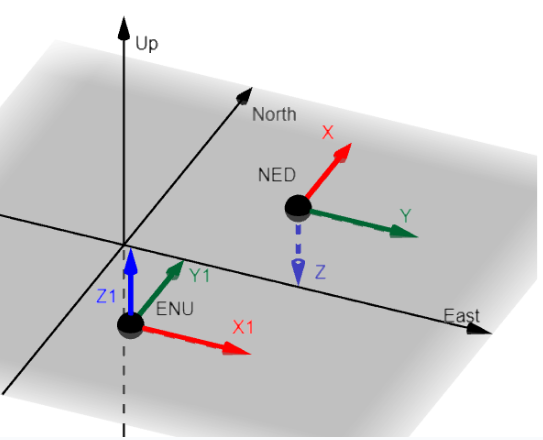
\includegraphics[width=0.5\textwidth, trim={0 0 0 0}, clip]{immagini/enu-ned.png}
	\caption{Rappresentazione dei sistemi di riferimento ENU e NED.}
	\label{fig:enu_ned}
\end{figure}
Per risolvere questo problema, è necessario convertire le coordinate da ENU a NED, applicando delle rotazioni. Osservando la Fig. \ref{fig:enu_ned}, è possibile notare che una delle combinazione di rotazioni che si possono applicare è: 90° sull'asse Z, 180° sull'asse Y. Quindi, sfruttando le matrici di rotazione Y e Z:
\[
R_y(\theta)=
\begin{bmatrix}
	\cos\theta & 0 & \sin\theta\\
	0 & 1 & 0\\
	-\sin\theta & 0 & \cos\theta
\end{bmatrix},
R_z(\psi)=
\begin{bmatrix}
	\cos\psi & -\sin\psi & 0\\
	\sin\psi & \cos\psi & 0\\
	0 & 0 & 1
\end{bmatrix}
\]
È possibile scrivere una matrice di conversione da ENU a NED:
\[
R_\mathrm{ENU\_NED}=R_y(\pi)\cdot R_z(\frac{\pi}{2})
\]
Essa deve essere applicata alla matrice di rotazione $R$, un valore ottenuto dalla funzione \texttt{solvePnP} di OpenCV che rappresenta come il marker è orientato rispetto alla camera. Questa funzione restituisce anche un vettore di traslazione $t$, che indica dove il marker di trova rispetto all'immagine. \\
\[
R_\mathrm{NED} = R\cdot R_\mathrm{ENU\_NED}
\]
Sia $p_m$ un vettore che rappresenta le coordinate a tre dimensioni di un punto nel mondo reale rispetto al marker; allora, le cordinate tridimensionali dello stesso punto nel sistema di riferimento della camera possiamo calcolarle in questo modo:
\[
p_c = R_\mathrm{NED}\cdot p_m+t
\]
Ma a noi interessa sapere l'opposto, ovvero trovare $p_m$:
\[
p_c = R_\mathrm{NED}\cdot p_m+t \Rightarrow p_c-t = R_\mathrm{NED}\cdot p_m \Rightarrow R_\mathrm{NED}^{-1}\cdot (p_c-t) = R_\mathrm{NED}^{-1}\cdot R_\mathrm{NED}\cdot p_m \Rightarrow
\]
\[
\Rightarrow p_m = R_\mathrm{NED}^{-1}\cdot (p_c-t)
\]
Una proprietà molto interessante della matrice di rotazione è che la sua inversa corrisponde alla sua trasposta: $R\cdot R^T=I$. Quindi è possibile semplificare la formula:
\[
p_m = R_\mathrm{NED}^T\cdot (p_c-t) = R_\mathrm{NED}^T\cdot p_c-R_\mathrm{NED}^T\cdot t
\]
In questo caso, il vettore $p_c$ punta all'origine della camera, quindi ha valore $\begin{bmatrix} 0 & 0 & 0 \end{bmatrix}^T$; di conseguenza, la formula diventa:
\[
p_m = R_\mathrm{NED}^T\cdot p_c-R_\mathrm{NED}^T\cdot t = R_\mathrm{NED}^T\cdot \begin{bmatrix} 0 & 0 & 0 \end{bmatrix}^T-R_\mathrm{NED}^T\cdot t = -R_\mathrm{NED}^T\cdot t
\]
Dentro questa formula manca ancora un'informazione, ovvero la posizione relativa del marker rispetto all'ambiente. Ognuno di essi si trova in una posizione diversa e nel calcolo della posizione questa informazione deve essere aggiunta. Per ogni marker, devono essere inserite le informazioni di posizione ENU, dimensione in metri e ID dentro un file json, che quindi descriverà l'ambiente della missione. \\
Definiamo $p_\mathrm{marker}$ il vettore posizione ENU del marker corrente, Allora, la formula precedente diventa:
\[
p_m = -R_\mathrm{NED}^T\cdot t + (R_\mathrm{ENU\_NED}\cdot p_\mathrm{marker})
\]
Riassumento:
\[
R_\mathrm{ENU\_NED}=R_y(\pi)\cdot R_z(\frac{\pi}{2})
\]
\[
R_\mathrm{NED} = R\cdot R_\mathrm{ENU\_NED}
\]
\[
\boxed{
		p_m = -R_\mathrm{NED}^T\cdot t + (R_\mathrm{ENU\_NED}\cdot p_\mathrm{marker})
}
\]
\subsection{Calcolo della posa}
Per descrivere l'orientamento del drone nello spazio tridimensionale è necessario analizzare la matrice $R_\mathrm{NED}$; in particolar modo, com'è composta \cite{kriz2006euler}. Partiamo dalla matrice di rotazione $R$. La possiamo descrivere attraverso le tre matrici di rotazione $X, Y, Z$:
\[
R_x(\phi)=
\begin{bmatrix}
	1 & 0 & 0\\
	0 & \cos\phi & -\sin\phi\\
	0  & \sin\phi & \cos\phi
\end{bmatrix},
R_y(\theta)=
\begin{bmatrix}
	\cos\theta & 0 & \sin\theta\\
	0 & 1 & 0\\
	-\sin\theta & 0 & \cos\theta
\end{bmatrix},
R_z(\psi)=
\begin{bmatrix}
	\cos\psi & -\sin\psi & 0\\
	\sin\psi & \cos\psi & 0\\
	0 & 0 & 1
\end{bmatrix}
\]
Adottando la convenzione ZYX, la matrice di rotazione $R$ si ottiene moltiplicando le matrici di rotazione nel seguente modo:
\[
R=R_z(\psi) \cdot R_y(\theta) \cdot R_x(\phi)
\]
Sviluppiamo prima il prodotto tra le matrici di rotazione $Y$ e $X$:
\[
R_yR_x=
\begin{bmatrix}
	\cos\theta & \sin\theta\sin\phi & \sin\theta\cos\phi\\
	0 & \cos\phi & -\sin\phi\\
	-\sin\theta & \cos\theta\sin\phi & \cos\theta\cos\phi
\end{bmatrix}
\]
Per poi unire anche la matrice relativa allo yaw:
\[
R=
\begin{bmatrix}
	\cos\psi & -\sin\psi & 0\\
	\sin\psi & \cos\psi & 0\\
	0 & 0 & 1
\end{bmatrix}
\cdot
\begin{bmatrix}
	\cos\theta & \sin\theta\sin\phi & \sin\theta\cos\phi\\
	0 & \cos\phi & -\sin\phi\\
	-\sin\theta & \cos\theta\sin\phi & \cos\theta\cos\phi
\end{bmatrix}=
\]
\[
\begin{bmatrix}
	\cos\psi\cos\theta &
	\cos\psi\sin\theta\sin\phi-\sin\psi\cos\phi &
	\cos\psi\sin\theta\cos\phi+\sin\psi\sin\phi\\
	\sin\psi\cos\theta &
	\sin\psi\sin\theta\sin\phi+\cos\psi\cos\phi &
	\sin\psi\sin\theta\cos\phi-\cos\psi\sin\phi\\
	-\sin\theta &
	\cos\theta\sin\phi &
	\cos\theta\cos\phi
\end{bmatrix}
\]
Abbiamo trovato $R$, quindi per calcolare $R_\mathrm{NED}$ basta moltiplicarla per la matrice di conversione $R_\mathrm{ENU\_NED}$:
\[
	R_\mathrm{NED} =
	R_\mathrm{ENU\_NED}
	\cdot
	\begin{bmatrix}
		\cos\psi\cos\theta &
		\cos\psi\sin\theta\sin\phi-\sin\psi\cos\phi &
		\cos\psi\sin\theta\cos\phi+\sin\psi\sin\phi\\
		\sin\psi\cos\theta &
		\sin\psi\sin\theta\sin\phi+\cos\psi\cos\phi &
		\sin\psi\sin\theta\cos\phi-\cos\psi\sin\phi\\
		-\sin\theta &
		\cos\theta\sin\phi &
		\cos\theta\cos\phi
	\end{bmatrix}
	=
\]
\[
\begin{bmatrix}
	0&1&0\\
	1&0&0\\
	0&0&-1
\end{bmatrix}
\cdot
\begin{bmatrix}
	\cos\psi\cos\theta &
	\cos\psi\sin\theta\sin\phi-\sin\psi\cos\phi &
	\cos\psi\sin\theta\cos\phi+\sin\psi\sin\phi\\
	\sin\psi\cos\theta &
	\sin\psi\sin\theta\sin\phi+\cos\psi\cos\phi &
	\sin\psi\sin\theta\cos\phi-\cos\psi\sin\phi\\
	-\sin\theta &
	\cos\theta\sin\phi &
	\cos\theta\cos\phi
\end{bmatrix}
=
\]
\[
\begin{bmatrix}
	\sin\psi\cos\theta &
	\sin\psi\sin\theta\sin\phi+\cos\psi\cos\phi &
	\sin\psi\sin\theta\cos\phi-\cos\psi\sin\phi\\
	\cos\psi\cos\theta &
	\cos\psi\sin\theta\sin\phi-\sin\psi\cos\phi &
	\cos\psi\sin\theta\cos\phi+\sin\psi\sin\phi\\
	\sin\theta &
	-\cos\theta\sin\phi &
	-\cos\theta\cos\phi
\end{bmatrix}
\]

\paragraph{Calcolo roll} L'angolo roll corrisponde alla misura di rotazione del sistema attorno all'asse X. In questo caso, l'asse da considerare non è l'asse X, ma l'asse Y, perché bisogna considerare che la matrice $R_\mathrm{NED}$ rappresenta la posizione e posa in coordinate NED, non ENU. Quindi, è possibile calcolarlo calcolando l'angolo $\theta$ in questo modo:
\[
\boxed{
	\theta = \arcsin({R_\mathrm{NED}}_{3,1}) = \arcsin(\sin\theta)
}
\]

\paragraph{Calcolo pitch} Sfruttando la stessa idea del calcolo del roll, si può calcolare il pitch. Essa corrisponde alla rotazione attorno all'asse Y, ma in questo caso, come spiegato precedentemente, corrisponde alla rotazione attorno all'asse X, ovvero l'angolo $\phi$. Di conseguenza:
\[
\boxed{
	\phi = \arctan(\frac{{R_\mathrm{NED}}_{3,2}}{{R_\mathrm{NED}}_{3,3}}) = \arctan(\frac{-\cos\theta\sin\phi}{-\cos\theta\cos\phi}) = \arctan(\frac{\sin\phi}{\cos\phi})
}
\]

\paragraph{Calcolo yaw} Infine, è possibile calcolare lo yaw calcolando $\psi$, ovvero la rotazione attorno all'asse Z. Guardando la matrice $R_\mathrm{NED}$, possiamo notare che:
\[
\psi=\arctan(\frac{{R_\mathrm{NED}}_{1,1}}{{R_\mathrm{NED}}_{2,1}})
\]
Dobbiamo fare attenzione ad un piccolo dettaglio, ovvero al senso di rotazione. Nel caso di roll e pitch cambiava l'asse, mentre in questo caso cambia il senso di rotazione, sempre per lo stesso motivo. Quindi, per risolvere questo conflitto dobbiamo inserire un segno $-$ nella formula per invertire il senso di rotazione e renderlo compatibile con lo yaw del flight controller:
\[
\boxed{
	\psi=\arctan(\frac{-{R_\mathrm{NED}}_{1,1}}{{R_\mathrm{NED}}_{2,1}})=\arctan(\frac{-\sin\psi\cos\theta}{\cos\psi\cos\theta})=\arctan(\frac{-\sin\psi}{\cos\psi})
}
\]

\subsection{Matrice di covarianza}
La matrice di covarianza permette di rappresentare l'incertezza delle variabili stimate dalla VO. Esse, insieme alla matrice di covarianza, vengono date in input al filtro di Kalman, che ne aggiornerà lo stato di conseguenza.

\subsubsection{Struttura}
Consideriamo il vettore di stato $\mathbf{s}$, una variabile aleatoria vettoriale composta in questo modo:
\[
\mathbf{s} =
\begin{bmatrix}
	x & y & z & \phi & \theta & \psi
\end{bmatrix}^{T}
\]
\begin{itemize}
	\item \(x,y,z\) rappresentano la posizione del drone nei tre assi cartesiani.
	\item\(\phi, \theta, \psi\) rappresentano rispettivamente roll, pitch e yaw.
\end{itemize}
Allora la matrice di covarianza $\mathbf{P}$ è formata in questo modo:
\[
\mathbf{P} =
\begin{bmatrix}
	\operatorname{Cov}(x,x) & \operatorname{Cov}(x,y) & \cdots & \operatorname{Cov}(x,\psi)\\
	\operatorname{Cov}(y,x) & \operatorname{Cov}(y,y) & \cdots & \operatorname{Cov}(y,\psi)\\
	\vdots & \vdots & \ddots & \vdots\\
	\operatorname{Cov}(\psi,x) & \operatorname{Cov}(\psi,y) & \cdots & \operatorname{Cov}(\psi,\psi)
\end{bmatrix}
\]
\\
Poiché la covarianza di una variabile con sé stessa coincide con la sua varianza:
\[
\operatorname{Cov}(x_i,x_i)
=\operatorname{Var}(x_i)
=\sigma_{x_i}^{2},
\]
la matrice può essere riscritta come:
\[
\mathbf{P} =
\begin{bmatrix}
	\sigma_x^2 & \operatorname{Cov}(x,y) & \cdots & \operatorname{Cov}(x,\psi) \\
	\operatorname{Cov}(y,x) & \sigma_y^2 & \cdots & \operatorname{Cov}(y,\psi) \\
	\vdots & \vdots & \ddots & \vdots \\
	\operatorname{Cov}(\psi,x) & \operatorname{Cov}(\psi,y) & \cdots & \sigma_\psi^2
\end{bmatrix}
\]
\\
Osservando il risultato, è possibile notare che questa è una matrice quadrata e simmetrica; questo vuol dire che per ogni coppia di indici (i,j), vale la relazione:
\[
P_{ij}=P_{ji}
\]
Questa proprietà deriva dalla simmetria della covarianza, per cui $\operatorname{Cov}(x_i,x_j)=\operatorname{Cov}(x_j,x_i)$.
\subsubsection{Calcoli}
In questa sezione vengono mostrati tutti i calcoli per ogni valore di posizione e posa.
Legenda (Fig. \ref{fig:dev_xy},\ref{fig:dev_z}):
\begin{itemize}
	\item $f$: distanza focale in pixel.
	\item $z_0$: asse ottico $z$ in metri.
	\item $O$: centro ottico.
	\item $pm$: piano immagine.
	\item $d'_x$: variazione nel piano immagine in pixel dell'asse X.
	\item $d_x$: variazione in metri di $d'_x$ nel mondo reale dell'asse X.
\end{itemize}
L'idea per calcolare la deviazione standard di ogni valore è trovare quanto esso cambia se l'immagine si sposta di 1 pixel.
\paragraph{Varianza x e y} Prendiamo in considerazione l'immagine in Fig. \ref{fig:dev_xy}; $d'_x$ rappresenta la variazione di $1px$ nel piano immagine $pm$, mentre $d_x$ rappresenta la distanza in metri rispetto alla variazione $d'_x$. \\
Osservango il disegno, è possibile notare che i triangoli $\triangle PM_0OPM_1$ e $\triangle L_0OL_1$ sono simili, dato che hanno due angoli congruenti; quindi, attraverso una proporzione è possibile dire che:
\[
\frac{d'_x}{f}=\frac{d_x}{z_0} \Rightarrow d_x=\frac{z_0}{f}\cdot d'_x
\]
Questa formula si chiama equazione prospettica. Sapendo che $d'_x=1px$, possiamo rappresentare la deviazione standard delle coordinate $x$ e $y$ in questo modo:
\[
\boxed{
	\sigma_x=\sigma_y=\frac{z_0}{f}\cdot 1px
}
\]
Infine, per ottenere la varianza basta elevare al quadrato la deviazione standard.

\begin{figure}[!htbp]
	\centering
	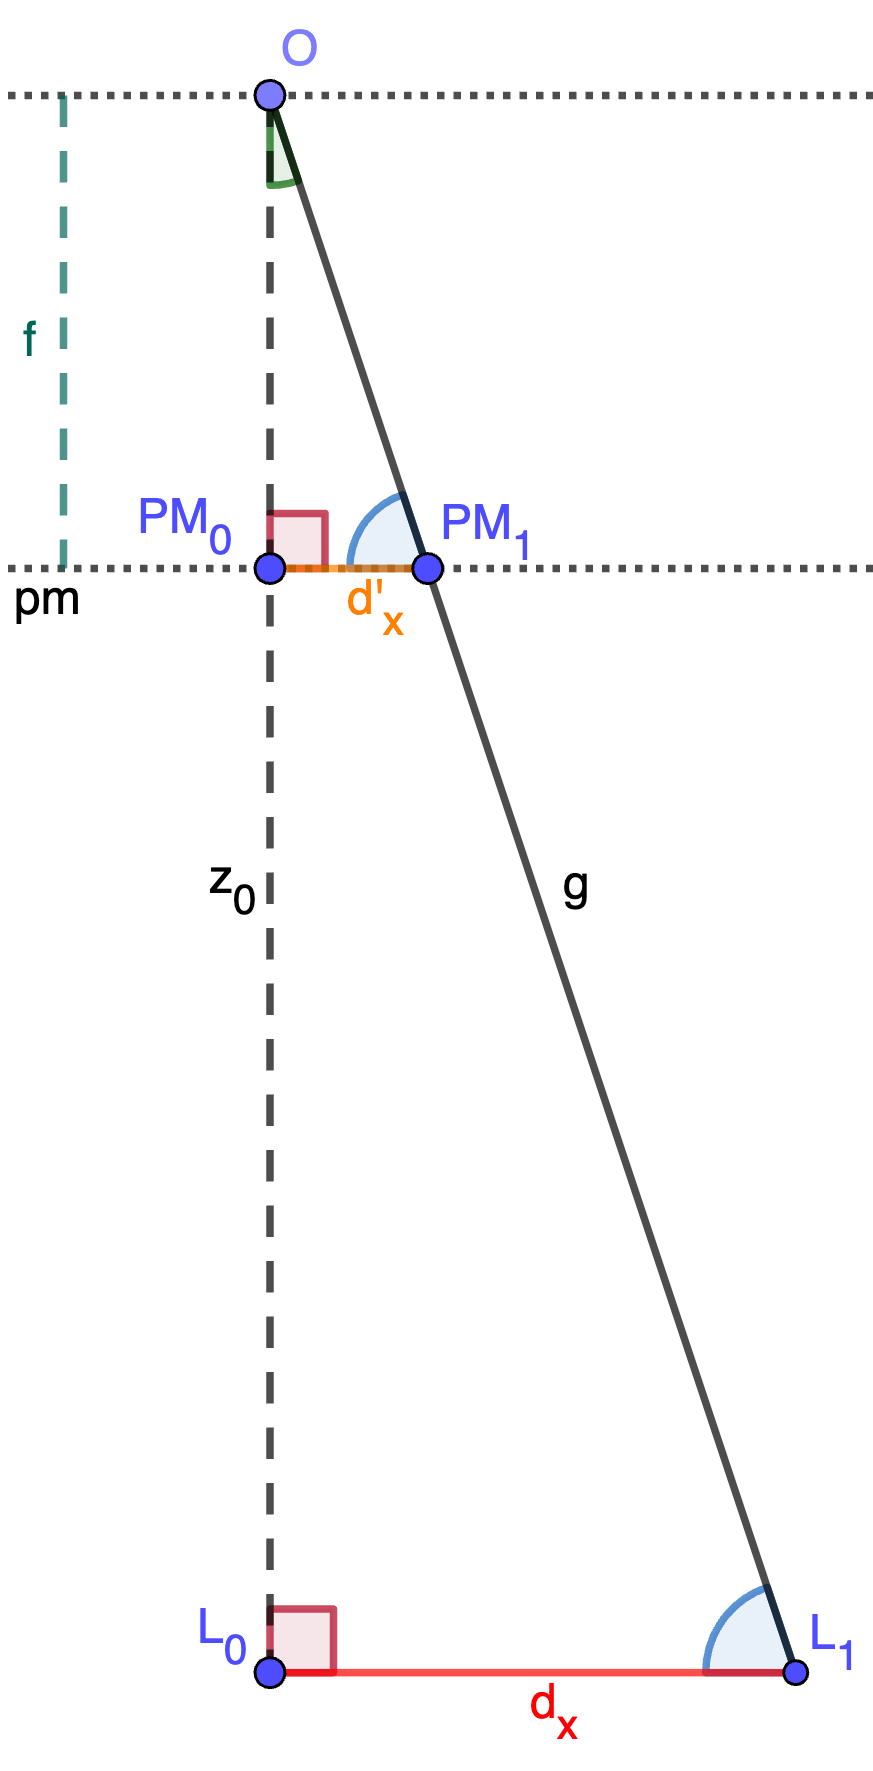
\includegraphics[width=0.3\textwidth, trim={0 0 0 0}, clip]{immagini/dev_xy.png}
	\caption{Disegno del calcolo della varianza delle coordinate $x$ e $y$.}
	\label{fig:dev_xy}
\end{figure}

\paragraph{Varianza z} La figura di riferimento è la Fig. \ref{fig:dev_z}. La deviazione standard è rappresentata dal segmento $d_z$. \\
Nella figura, possiamo notare che i triangoli $\triangle L_1AL_3$ e $\triangle L_0OL_3$ sono simili, dato che hanno due angoli congruenti. Attraverso lo stesso ragionamento, possiamo dire che anche i triangoli $\triangle FOPM_1$ e $\triangle L_0OL_3$ sono simili; quindi $\triangle FOPM_1$ e $\triangle L_1AL_3$ sono simili. Grazie a questo, possiamo scrivere la seguente proporzione:
\[
\frac{d_z}{d_x}=\frac{f}{\frac{l_{im}}{2}+d'_x} \Rightarrow d_z=\frac{f}{\frac{l_{im}}{2}+d'_x}\cdot d_x
\]
Il valore $d_x$ lo abbiamo calcolato nel paragrafo precedente, ed è uguale a $d_x=\frac{z_0}{f}\cdot d'_x$; mentre $d'_x=\frac{1}{2}px$, mezzo pixel per ogni lato del triangolo nel disegno. Quindi, sostituendo i valori, l'equazione risulta:
\[
d_z=\frac{f}{\frac{l_{im}}{2}+d'_x}\cdot d_x=\frac{f}{\frac{l_{im}}{2}+d'_x}\cdot\frac{z_0}{f}\cdot\frac{1}{2}px=\frac{z_0\cdot\frac{1}{2}px}{\frac{l_{im}}{2}+d'_x} = \frac{z_0\cdot\frac{1}{2}px}{\frac{l_{im}}{2}+\frac{1}{2}px} = \frac{z_0}{l_{im}+1px}
\]
Dato che il valore $l_{im}$ ha ordine di grandezza di qualche centinaio di pixel, è possibile eseguire la seguente approssimazione:
\[
\boxed{
	d_z=\frac{z_0}{l_{im}+1px} \approx \frac{z_0}{l_{im}}
}
\]
\begin{figure}[!htbp]
	\centering
	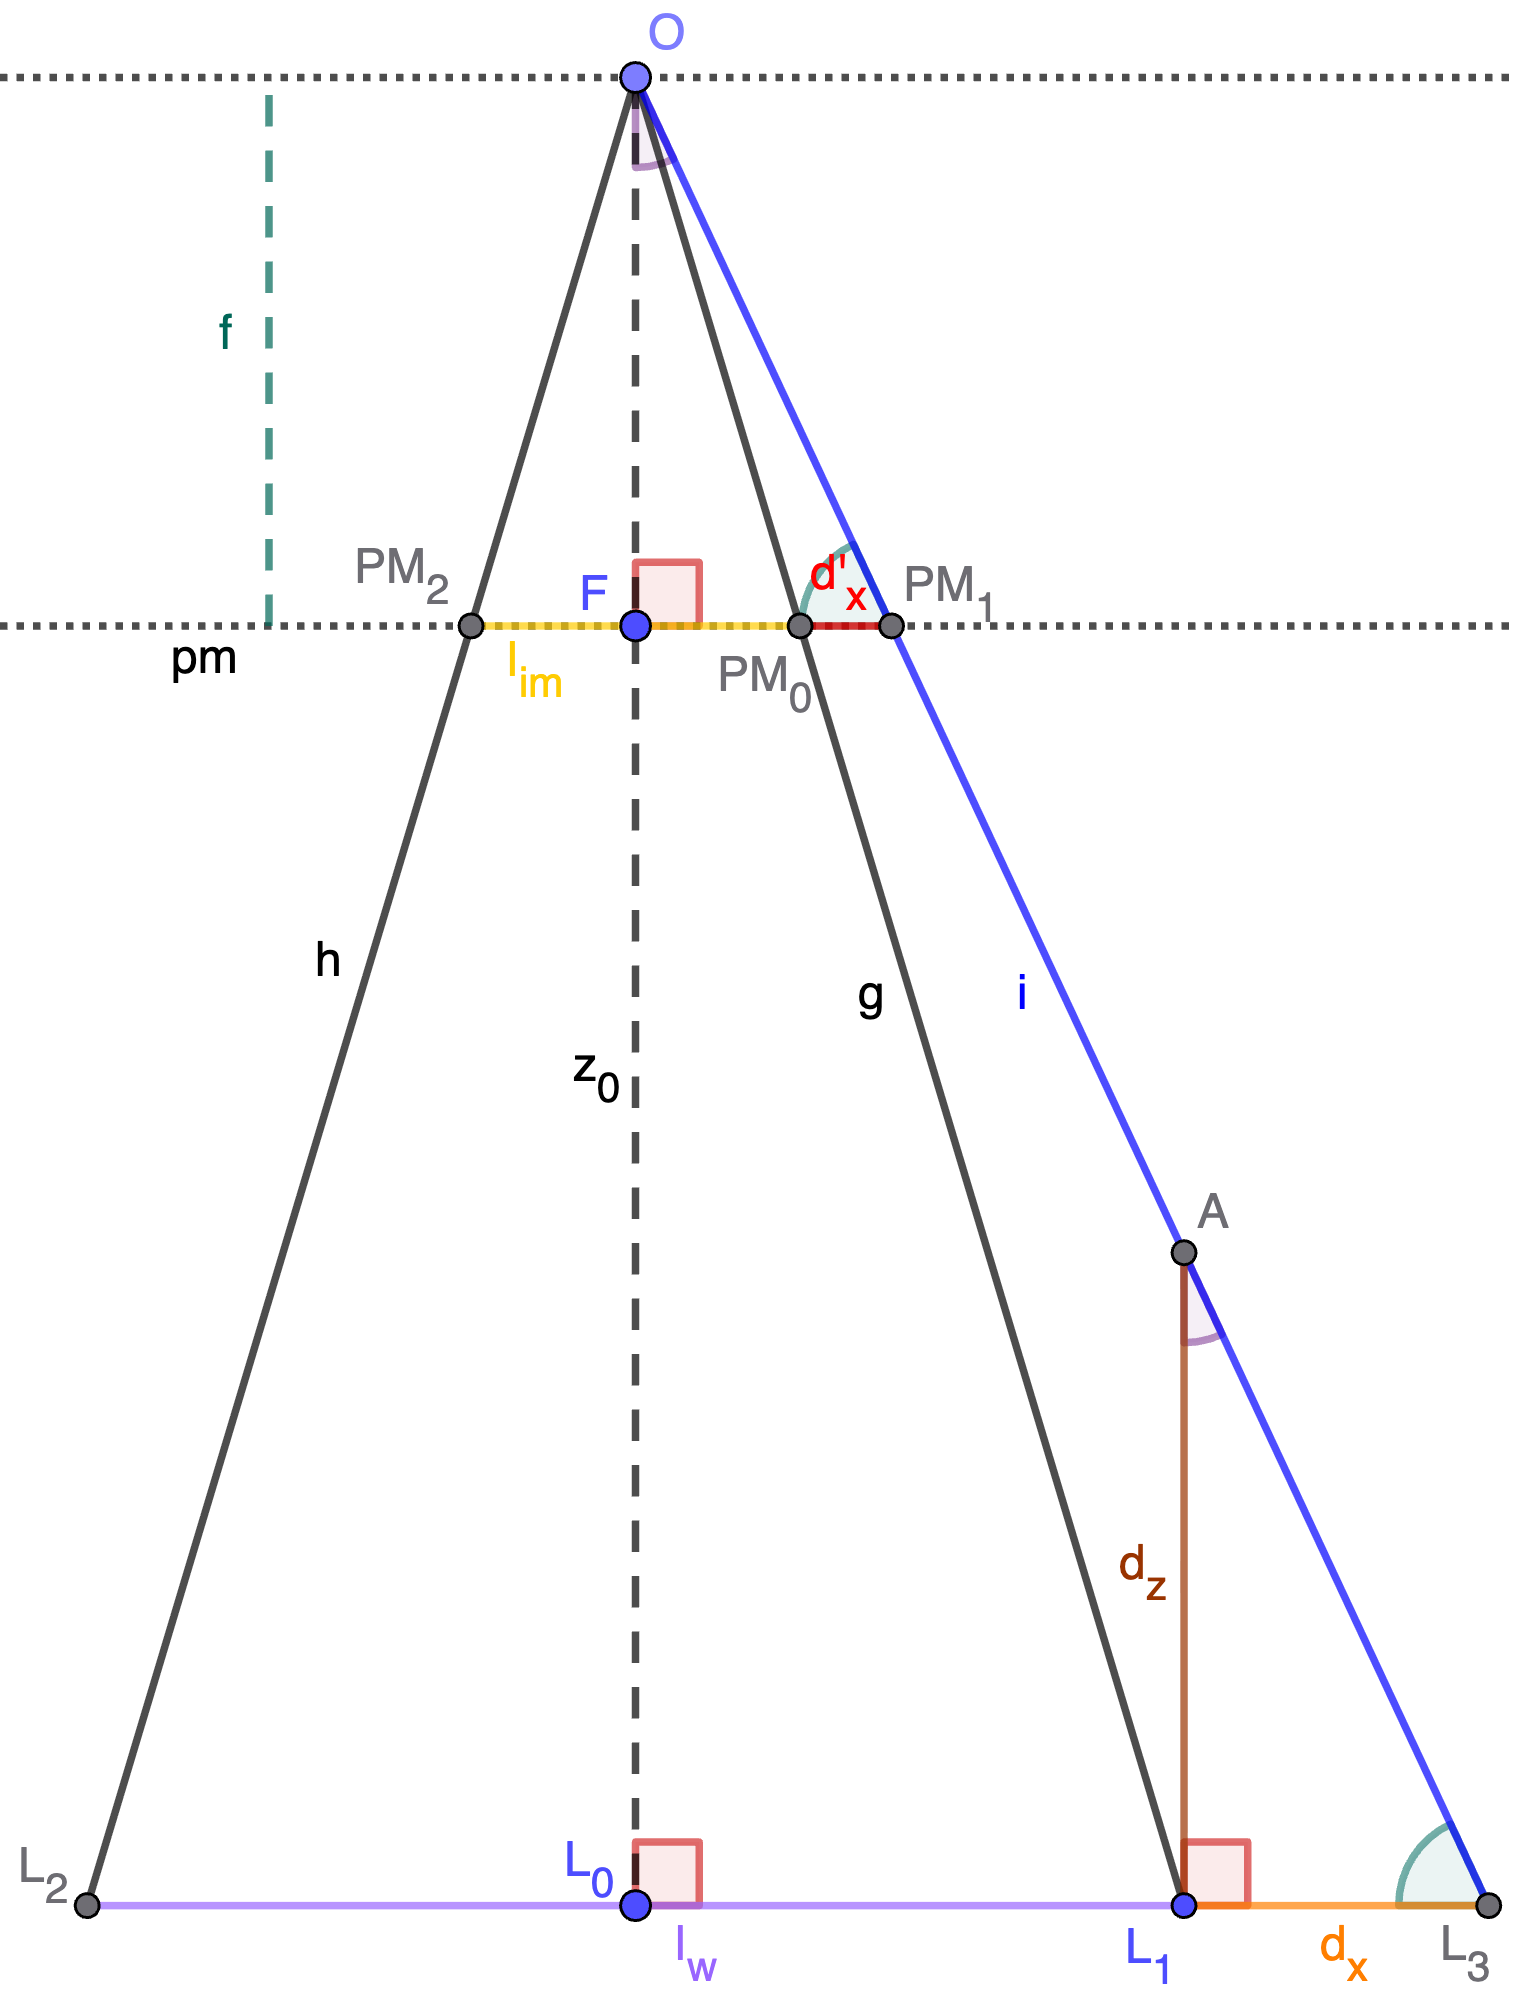
\includegraphics[width=0.4\textwidth, trim={0 0 0 0}, clip]{immagini/dev_z.png}
	\caption{Disegno del calcolo della varianza della coordinata $z$.}
	\label{fig:dev_z}
\end{figure}
\paragraph{Varianza roll e pitch} La deviazione standard è rappresentata dall'angolo $\gamma$, visibile in Fig. \ref{fig:dev_roll_pitch}. \\
Calcolare $d_x$ è molto semplice:
\[
d_x=m\cdot\tan(\gamma) \Rightarrow \tan(\gamma)=\frac{d_x}{m}
\]
Noi sappiamo che $d_x=1px$ e $m=\sqrt{f^2+(\frac{l_{im}}{2})^2}$, quindi:
\[
\tan(\gamma)=\frac{1}{\sqrt{f^2+(\frac{l_{im}}{2})^2}} \Rightarrow \gamma =\arctan(\frac{1}{\sqrt{f^2+(\frac{l_{im}}{2})^2}})
\]
Per valori di $x$ tendenti a 0, $\arctan(x) \approx x$, quindi:
\[
\boxed{
	\gamma=arctan(\frac{1}{\sqrt{f^2+(\frac{l_{im}}{2})^2}}) \approx \frac{1}{\sqrt{f^2+(\frac{l_{im}}{2})^2}}
}
\]

\begin{figure}[!htbp]
	\centering
	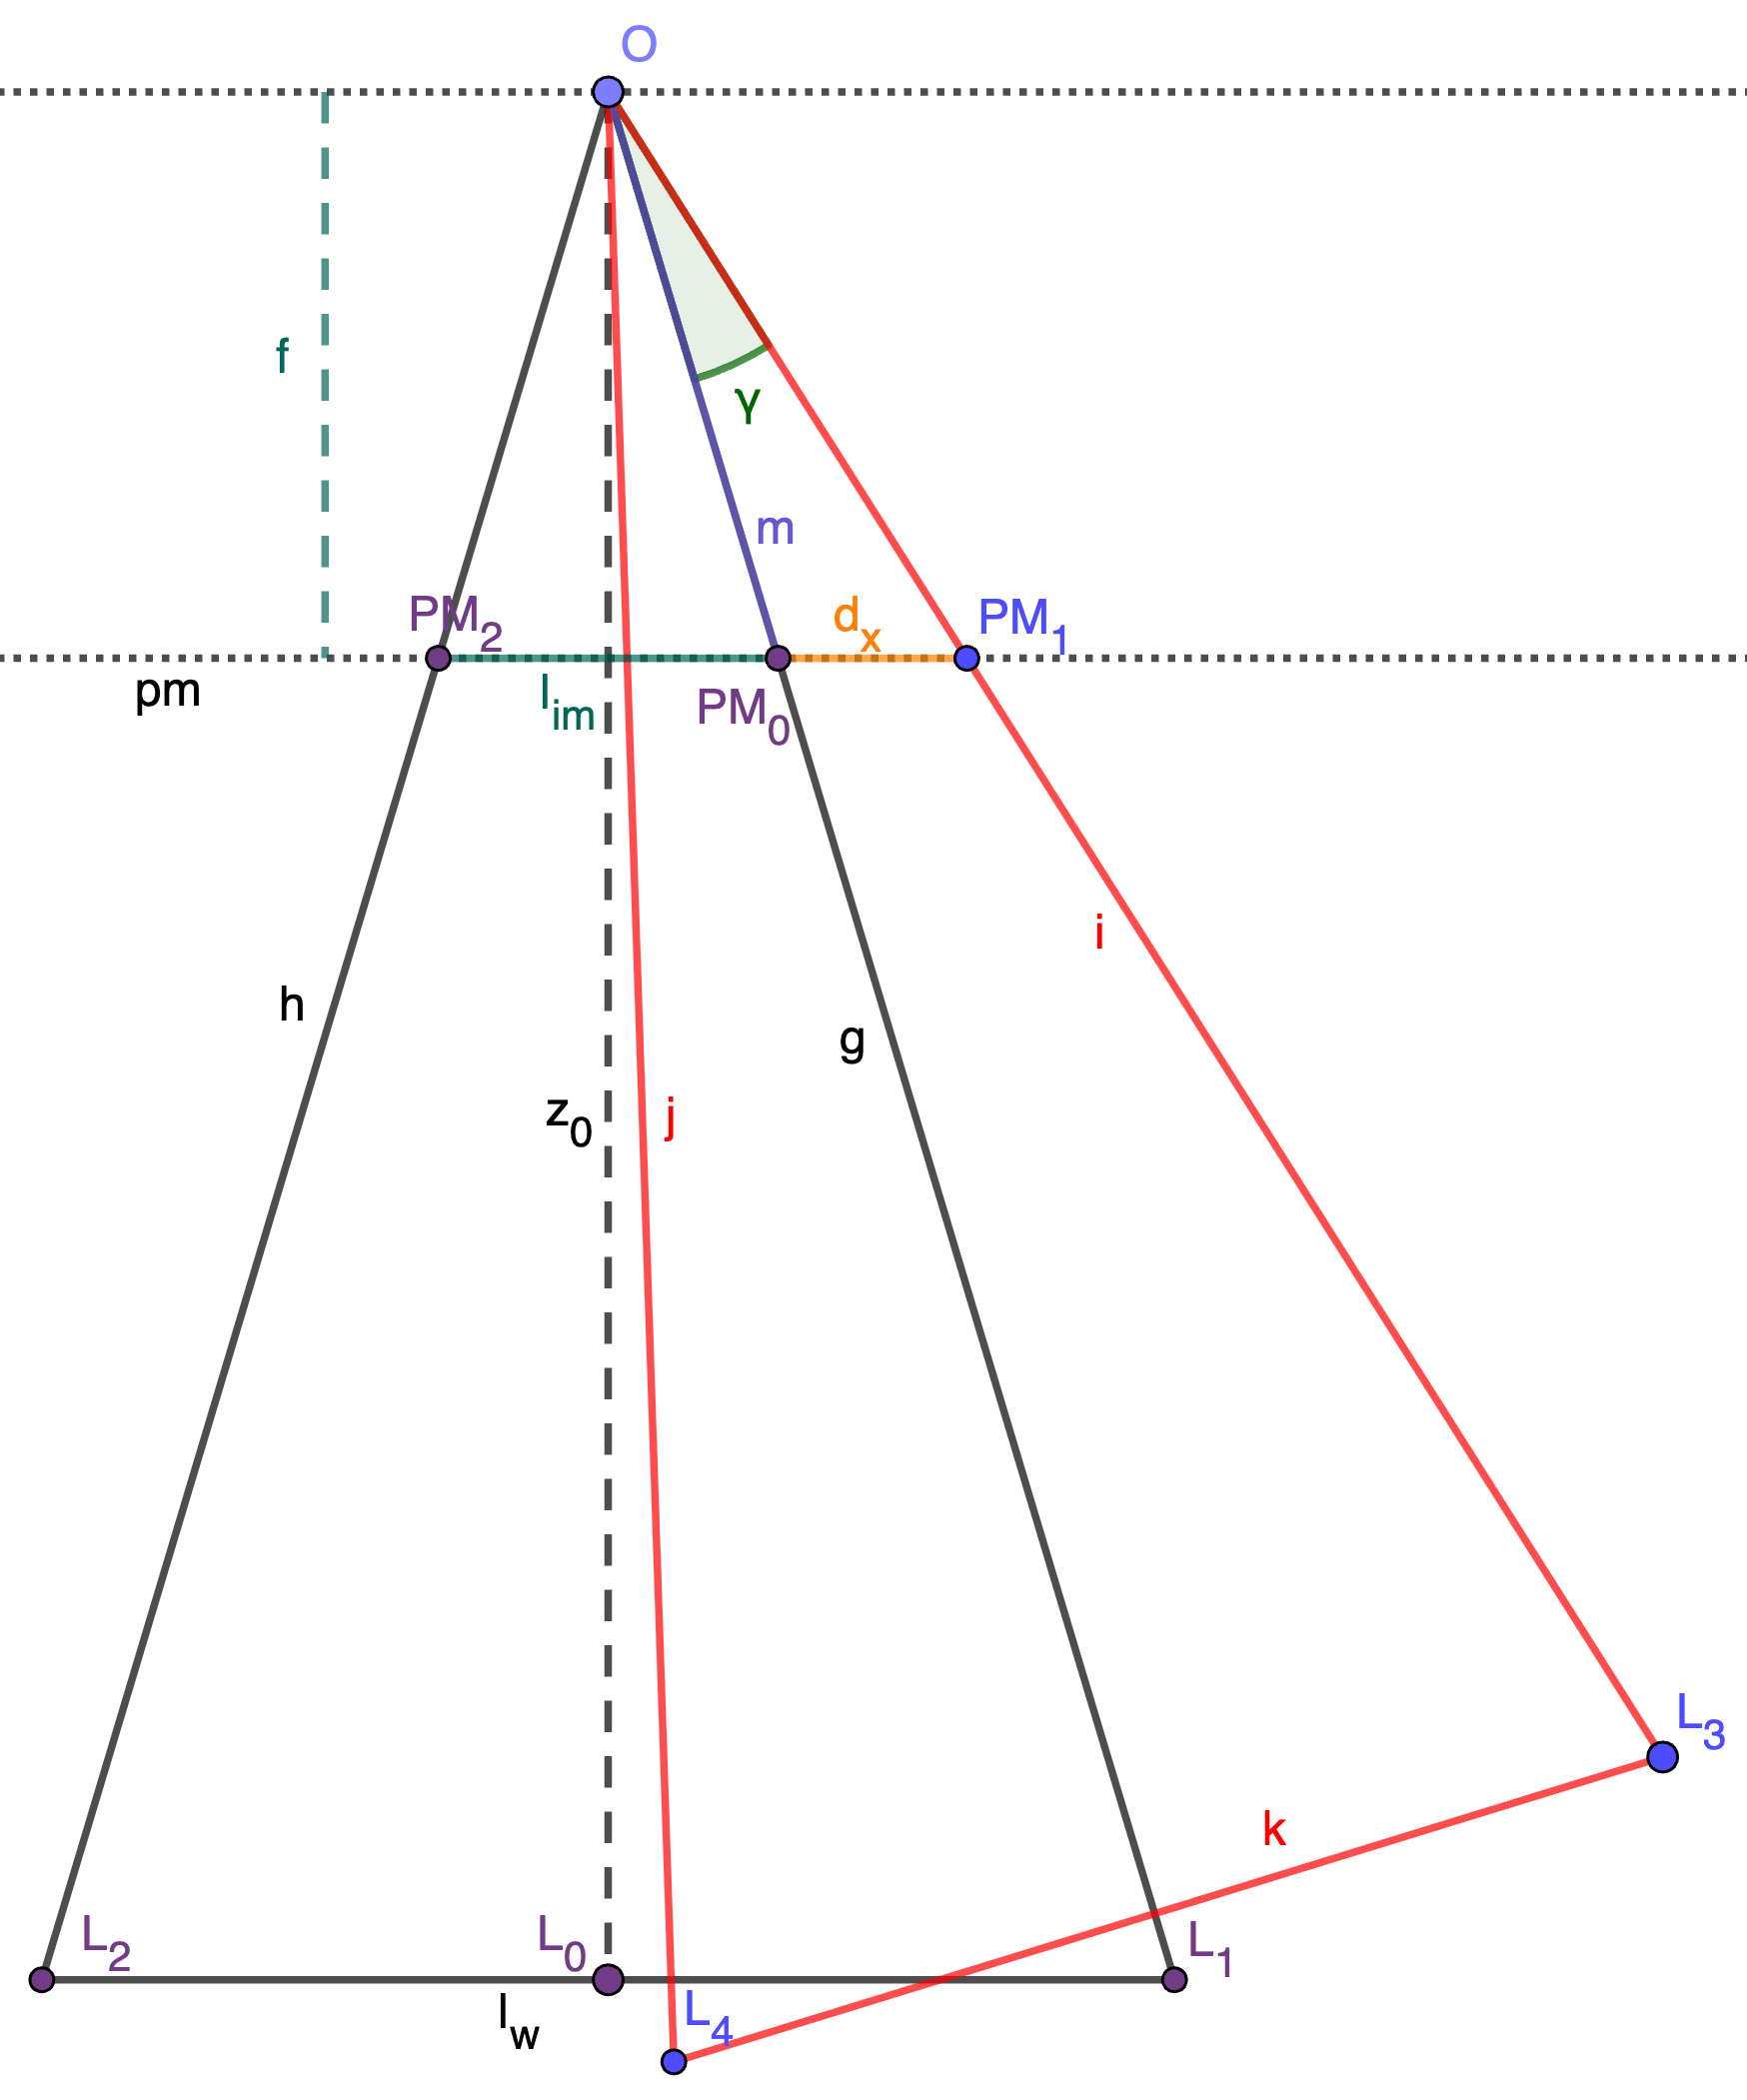
\includegraphics[width=0.5\textwidth, trim={0 0 0 0}, clip]{immagini/dev_roll_pitch.png}
	\caption{Disegno del calcolo della varianza degli angoli roll e pitch.}
	\label{fig:dev_roll_pitch}
\end{figure}

\paragraph{Varianza yaw} Nel disegno in Fig. \ref{fig:dev_yaw}, l'angolo $\alpha$ rappresenta la deviazione standard dello yaw. \\
Noi sappiamo che:
\[
 d_x=c\cdot\tan(\alpha)
\]
\[
c=\frac{\sqrt{l_0^2+l_0^2}}{2}=\frac{\sqrt{2}\cdot l_0}{2}=\frac{l_0}{\sqrt{2}}
\]
Quindi, sfruttando le formule precedenti, possiamo trovare $\alpha$ isolandolo dal $\tan(\alpha)$:
\[
tan(\alpha)=\frac{d_x}{c}=d_x\cdot\frac{\sqrt{2}}{l_0}
\]
Dalle premesse sappiamo che $d_x=1px$, quindi:
\[
\tan(\alpha)=\frac{\sqrt{2}}{l_0} \Rightarrow \alpha=\arctan(\frac{\sqrt{2}}{l_0})
\]
Dato che l'argomento di $\arctan(\frac{\sqrt{2}}{l_0})$ tente a 0, è possibile approssimare:
\[
\boxed{
	\alpha=\arctan(\frac{\sqrt{2}}{l_0})\approx \frac{\sqrt{2}}{l_0}
}
\]

\begin{figure}[!htbp]
	\centering
	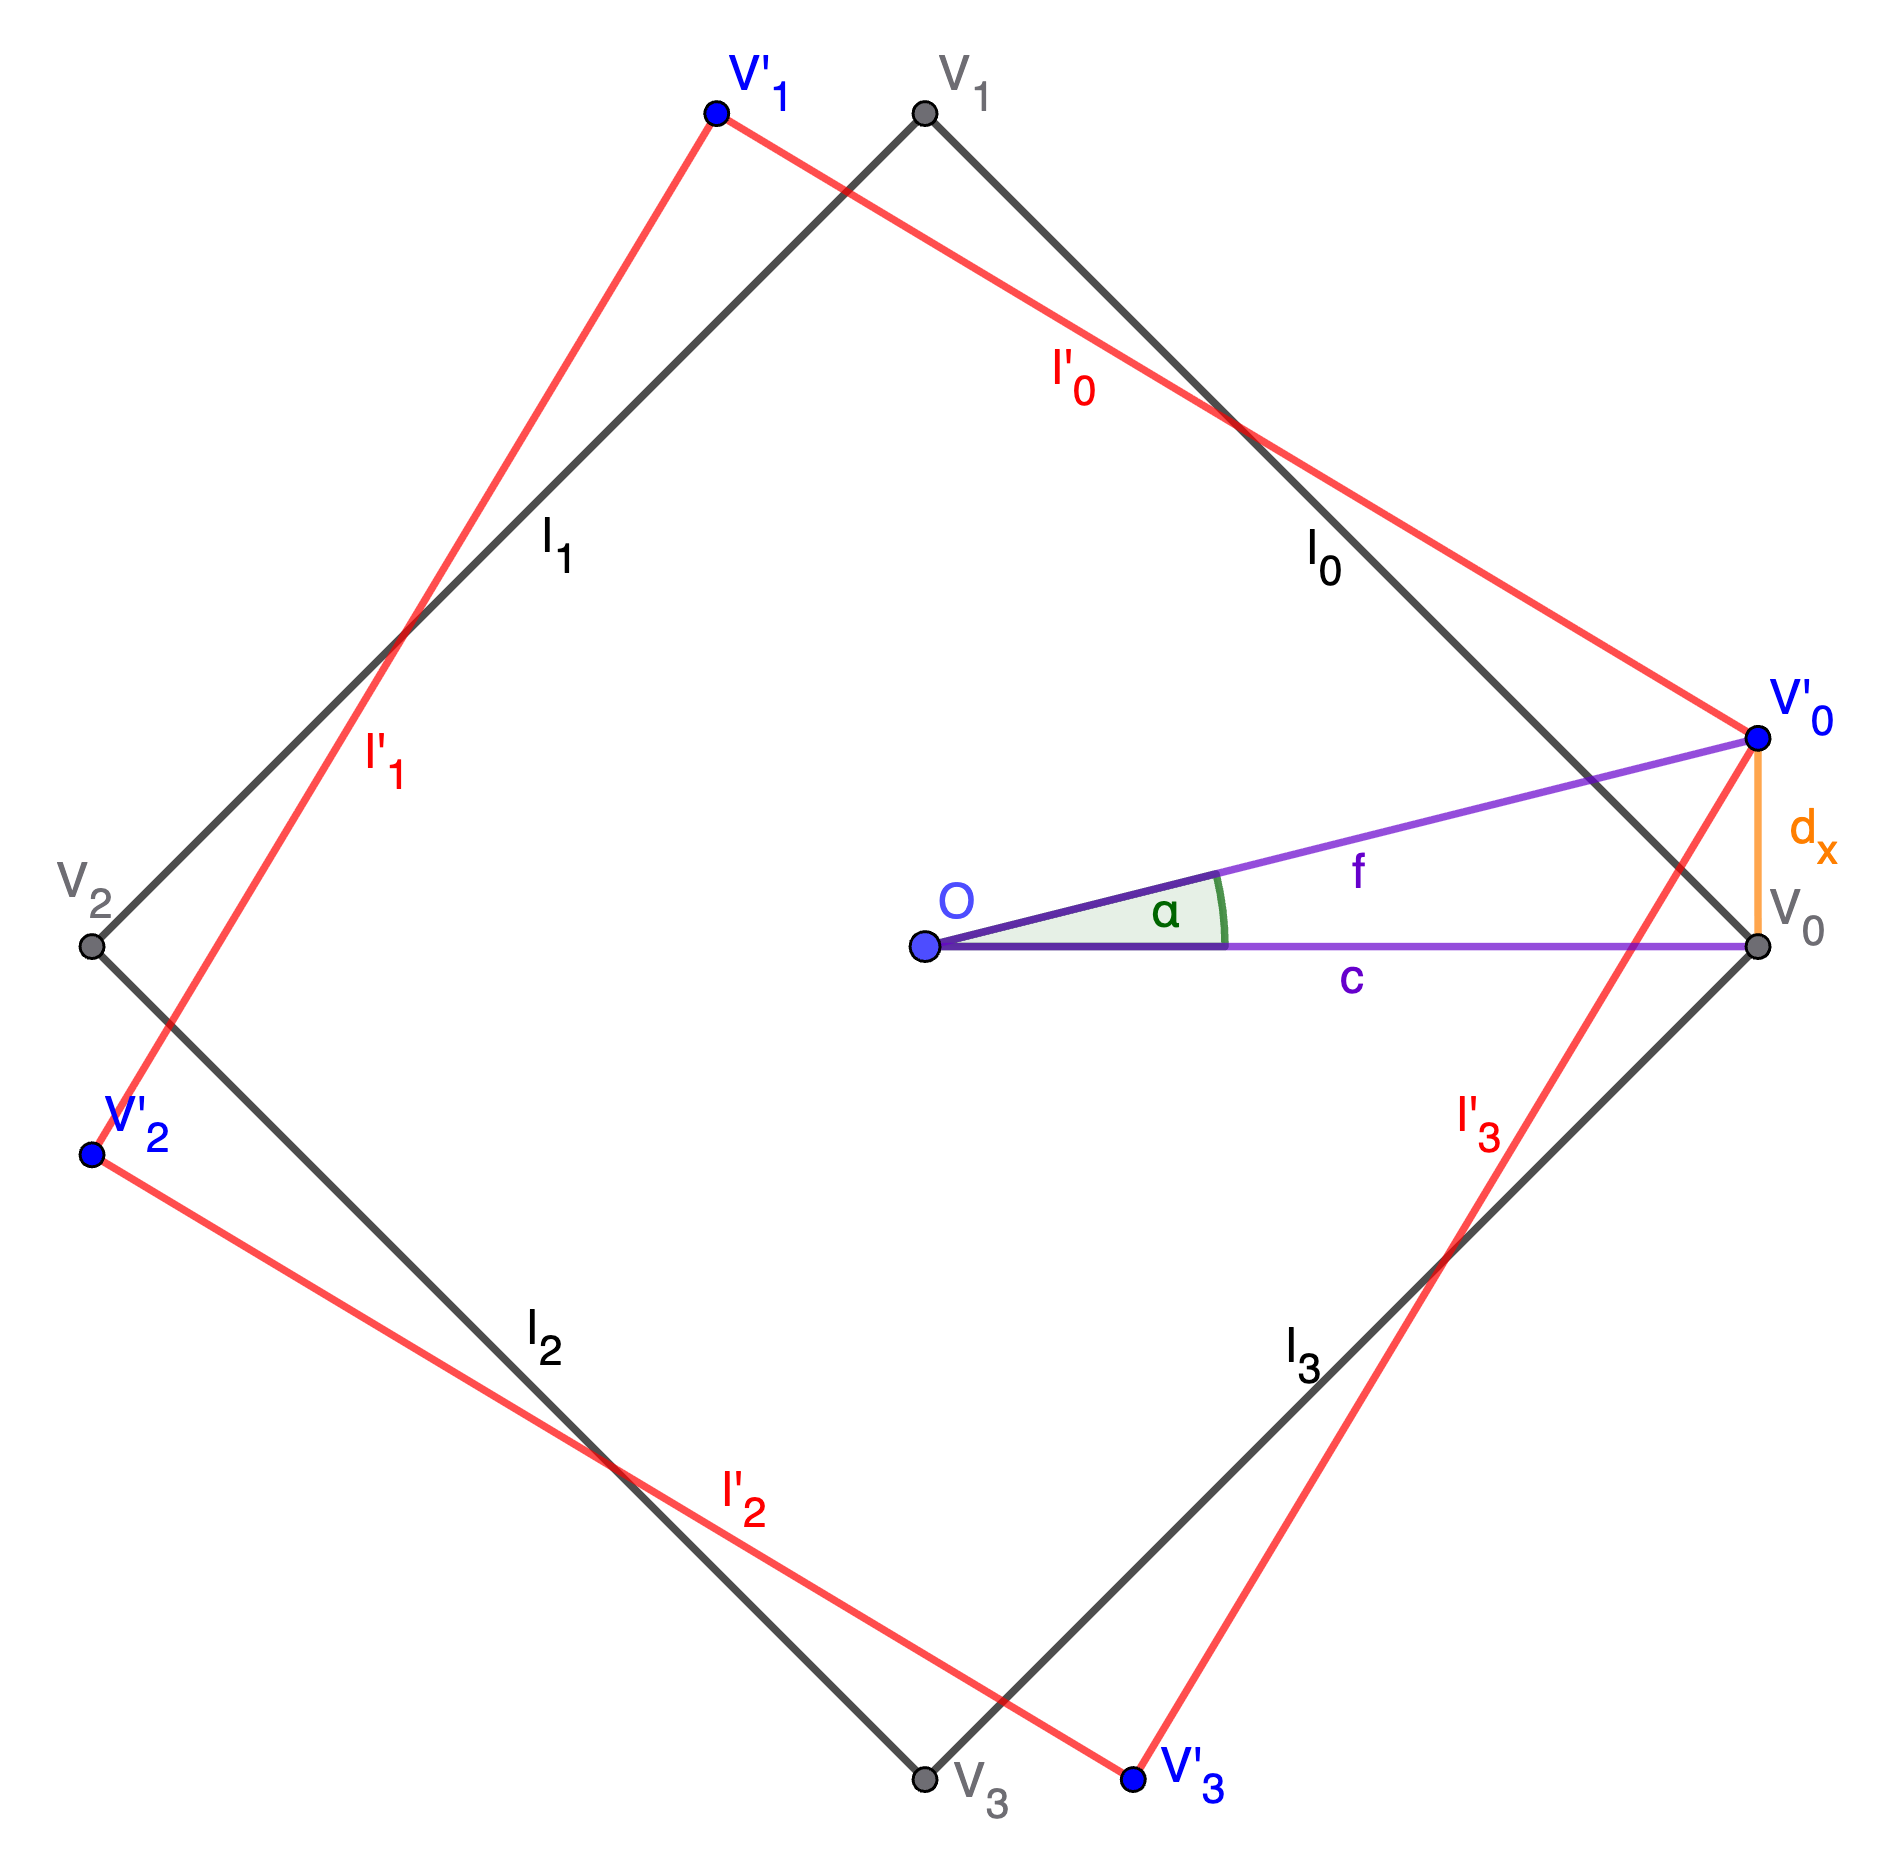
\includegraphics[width=0.5\textwidth, trim={0 0 0 0}, clip]{immagini/dev_yaw.png}
	\caption{Disegno del calcolo della varianza dell'angolo yaw.}
	\label{fig:dev_yaw}
\end{figure}
\subsubsection{Conclusioni}
Per concludere, nel modulo \texttt{mavsdk} la matrice di covarianza viene rappresentata attraverso la classe \texttt{mavsdk.mocap.Covariance}. Essa vuole come parametro \texttt{NaN}, se la matrice di covarianza è sconosciuta; opppure il triangolo superiore destro della matrice, dato che è simmetrica. Ecco confronto della matrice completa contro quella compressa:
\[
\mathbf{P} =
\begin{bmatrix}
	\sigma_x^2 & \operatorname{Cov}(x,y) & \cdots & \operatorname{Cov}(x,\psi) \\
	\operatorname{Cov}(y,x) & \sigma_y^2 & \cdots & \operatorname{Cov}(y,\psi) \\
	\vdots & \vdots & \ddots & \vdots \\
	\operatorname{Cov}(\psi,x) & \operatorname{Cov}(\psi,y) & \cdots & \sigma_\psi^2
\end{bmatrix}
\Rightarrow
\mathbf{P} =
\begin{bmatrix}
	\sigma_x^2 & \operatorname{Cov}(x,y) & \cdots & \operatorname{Cov}(x,\psi) \\
			 & \sigma_y^2 & \cdots & \operatorname{Cov}(y,\psi) \\
	 &  & \ddots & \vdots \\
	&  &  & \sigma_\psi^2
\end{bmatrix}
\]
La matrice originale ha $6x6$ valori, mentre quella compressa ne ha $21$. \\ \\
Infine, possiamo assumere che gli errori di misura dei sensori siano indipendenti tra loro. La covarianza tra due variabili indipentendi è zero, quindi la matrice finale sarà:
\[
\boxed{
	\mathbf{P} =
	\begin{bmatrix}
		\sigma_x^2 & 0 & \cdots & 0 \\
		& \sigma_y^2 & \cdots & 0 \\
		&  & \ddots & \vdots \\
		&  &  & \sigma_\psi^2
	\end{bmatrix}
}
\]

\subsection{Camera}
\label{sec:vo:camera}
\subsubsection{Scelta camera}
La scelta della camera ha un ruolo importantissimo per il sistema. I fattori importanti da considerare sono: la compatibilità con il Raspberry Pi 3, la risoluzione della camera, il FOV (Field of View) e il tipo di otturatore. I primi tre valori sono relativamente facili da soddisfare e dipendono fortemente dall'ambiente di volo; mentre l'ultimo è un fattore molto critico che richiede un pò di attenzione e approfondimento. \\
Esistono due tecnologie di otturatori: global shutter e rolling shutter. Nel primo caso, l'intera imagine viene acquisita nello stesso istante, pixel per pixel; mentre nel secondo caso, l'immagine viene acquisita riga per riga, quindi non nello stesso istante. Un esempio di rolling shutter camera è il Raspberry Pi Camera Module 2\footnote{\url{https://www.raspberrypi.com/products/camera-module-v2/}}. Il problema di quest'ultima tecnologia è che in caso di movimento laterale, l'immagine risulterà distorta (esempio in Fig. \ref{fig:rolling_shutter1}, \ref{fig:rolling_shutter2}. Notare come le linee dritte del pavimento si siano distorte). 
\begin{figure}[!htbp]
	\centering
	\begin{subfigure}[b]{0.48\textwidth}
		\centering
		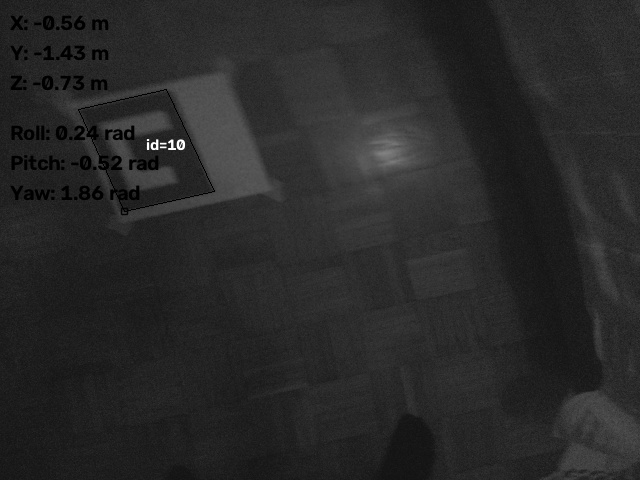
\includegraphics[width=\textwidth, trim={0 0 0 0}, clip]{immagini/rolling_shutter_1.jpg}
		\caption{Esempio distorsione verso destra.}
		\label{fig:rolling_shutter1}
	\end{subfigure}
	\hfill % Crea lo spazio orizzontale tra le due immagini
	\begin{subfigure}[b]{0.48\textwidth}
		\centering
		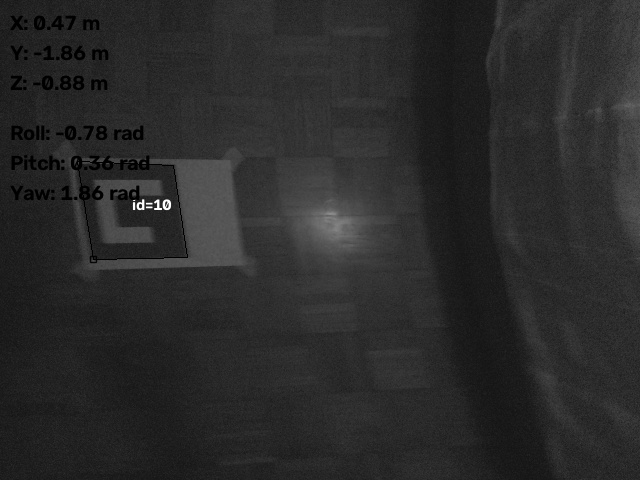
\includegraphics[width=\textwidth, trim={0 0 0 0}, clip]{immagini/rolling_shutter_2.jpg}
		\caption{Esempio distorsione verso sinistra.}
		\label{fig:rolling_shutter2}
	\end{subfigure}
	\caption{Distorsioni dovute dalla camera rolling shutter Raspberry Pi Camera Module 2. Le immagini sono state scattate nello stesso ambiente, con lo stesso pavimento.}
	\label{fig:rolling_shutter_all}
\end{figure}
Questa distorsione porta l'algoritmo della VO a restituire valori completamente sbagliati. Un esempio pratico dell'effetto di questo problema si può notare confrontanto i log nelle Fig. \ref{fig:log_rolling_shutter} e \ref{fig:log_global_shutter}; nella Fig. \ref{fig:log_rolling_shutter} è facile notare come ci siano degli sbalzi improvvisi, dovuti dalle immagini distorte della camera rolling shutter. Gli sbalzi si presentano soprattutto attraverso gli spostamenti laterali; infatti è proprio questo movimento che permette di accentuare questo fenomeno.
\begin{figure}[!htbp]
	\centering
	\begin{subfigure}[b]{0.48\textwidth}
		\centering
		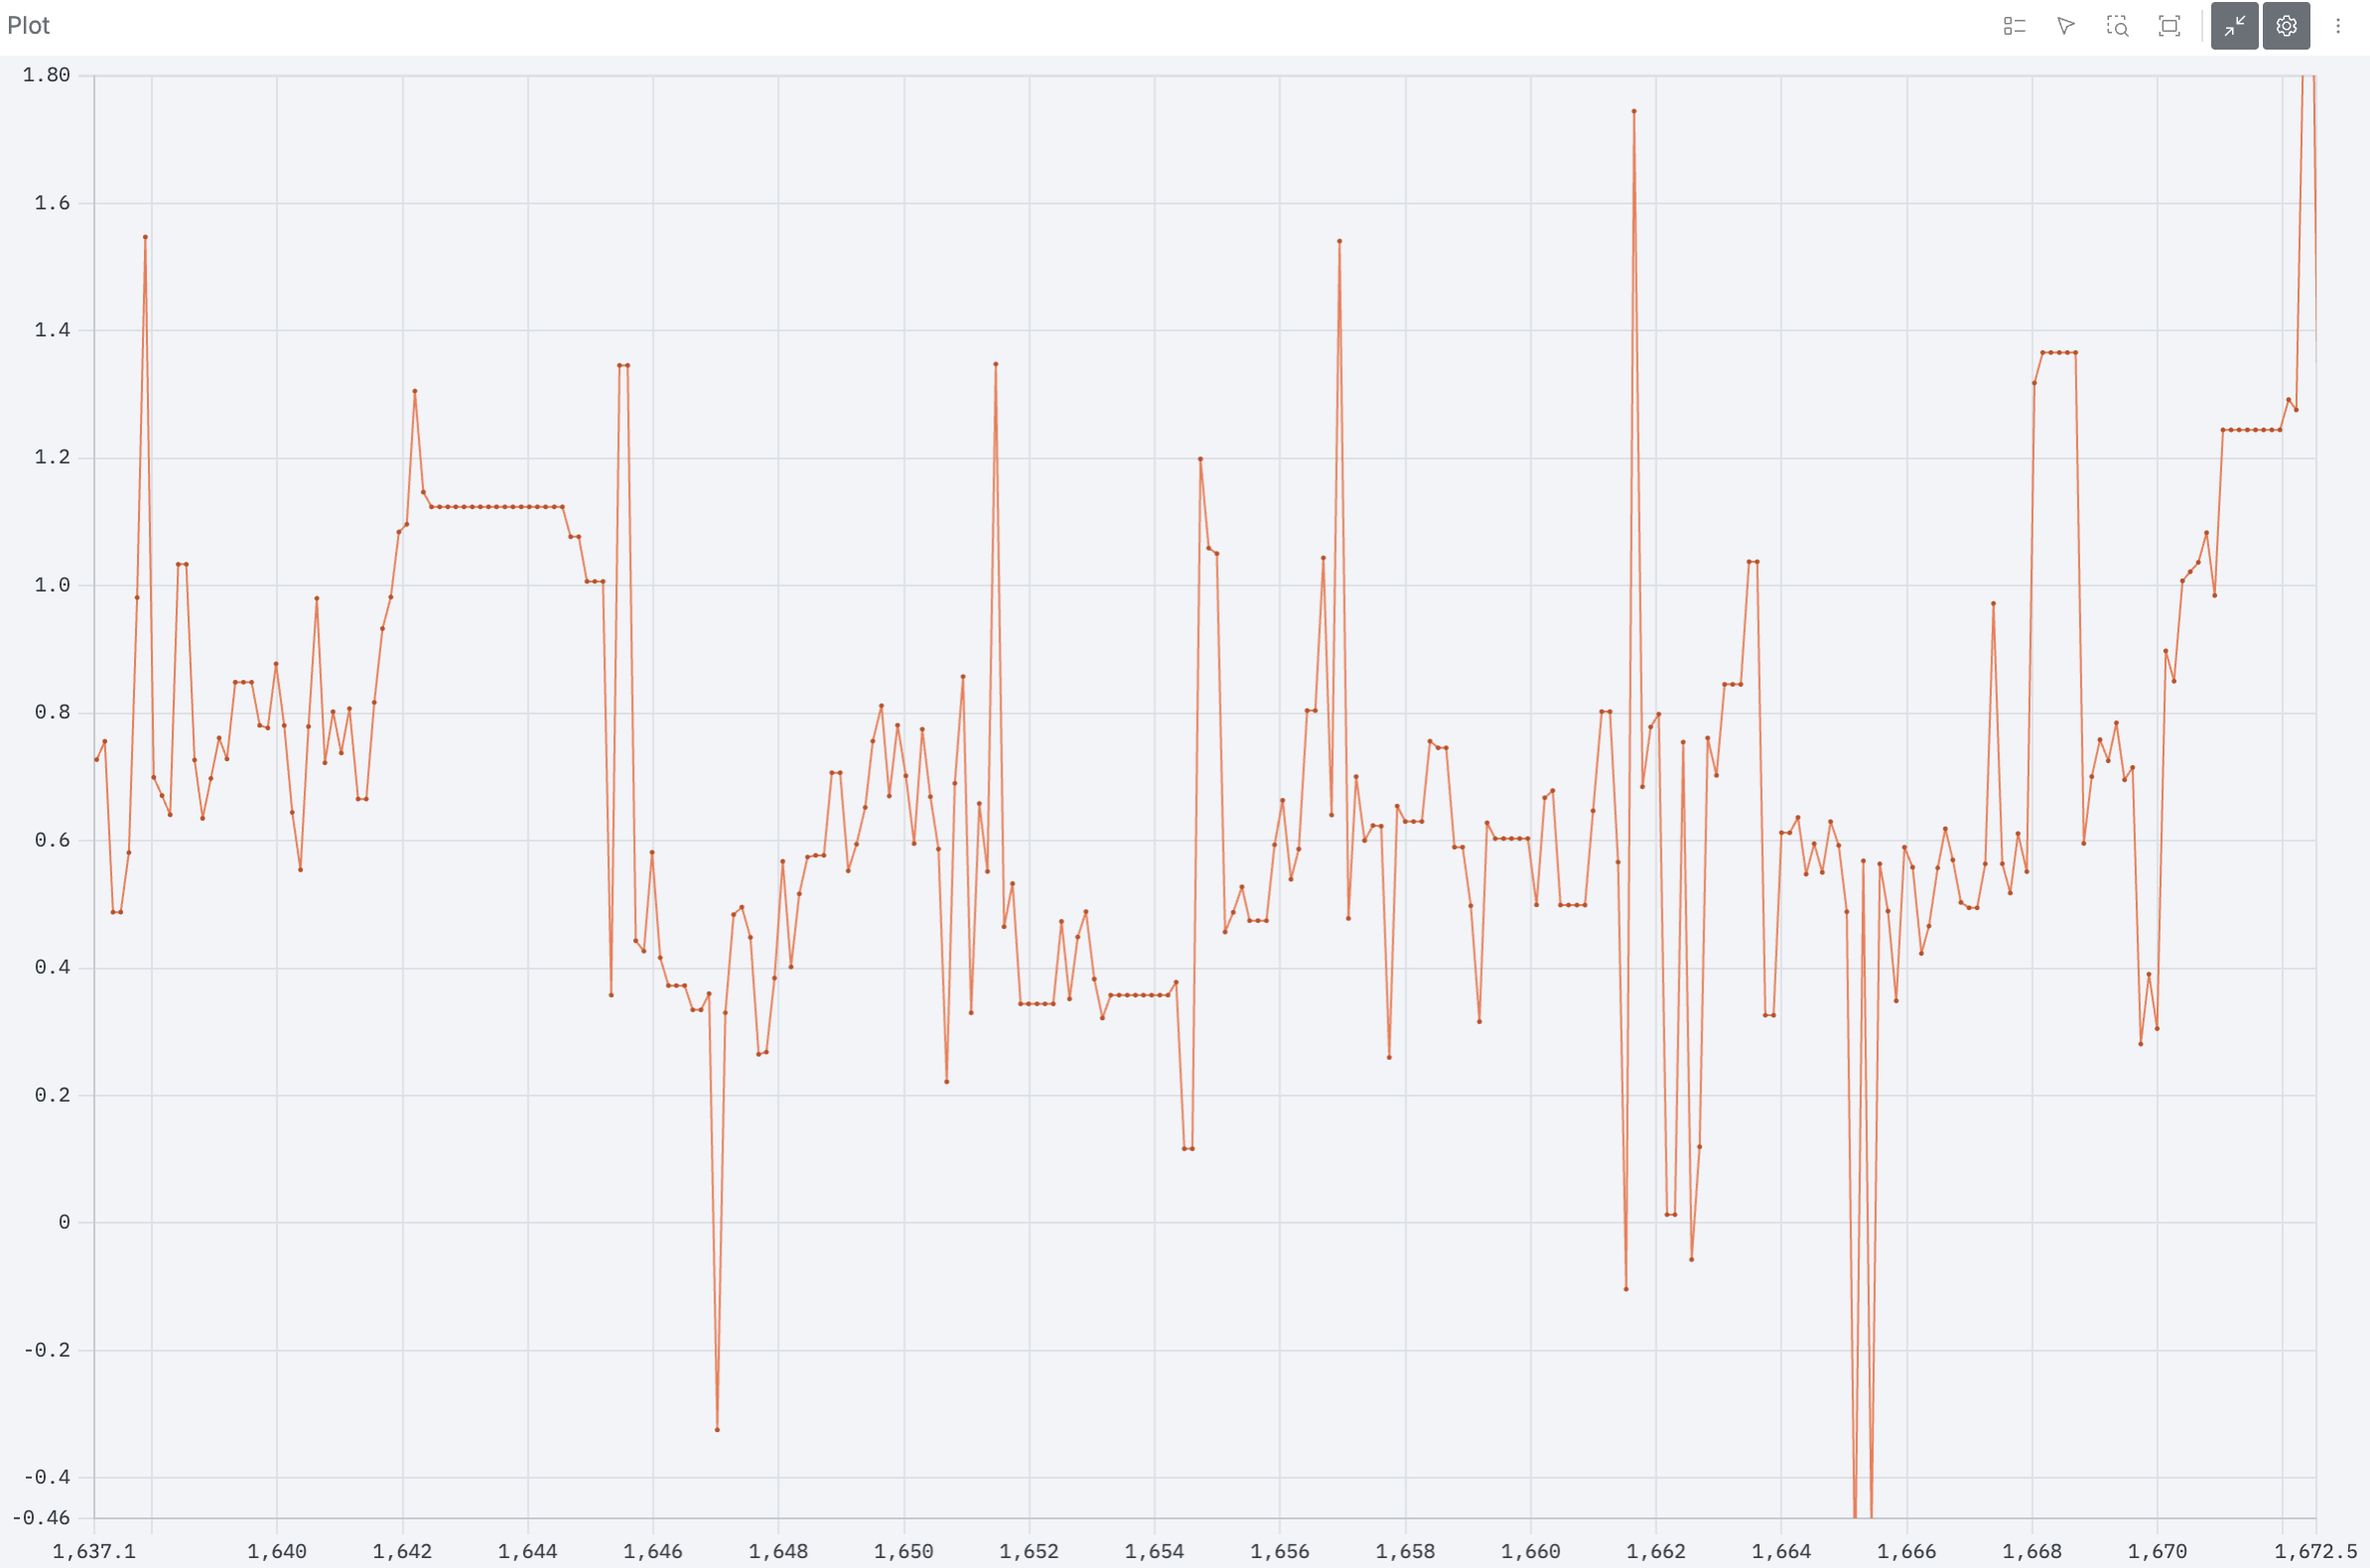
\includegraphics[width=\textwidth, trim={0 0 0 0}, clip]{immagini/log_distorto.png}
		\caption{Log con camera rolling shutter.}
		\label{fig:log_rolling_shutter}
	\end{subfigure}
	\hfill % Crea lo spazio orizzontale tra le due immagini
	\begin{subfigure}[b]{0.48\textwidth}
		\centering
		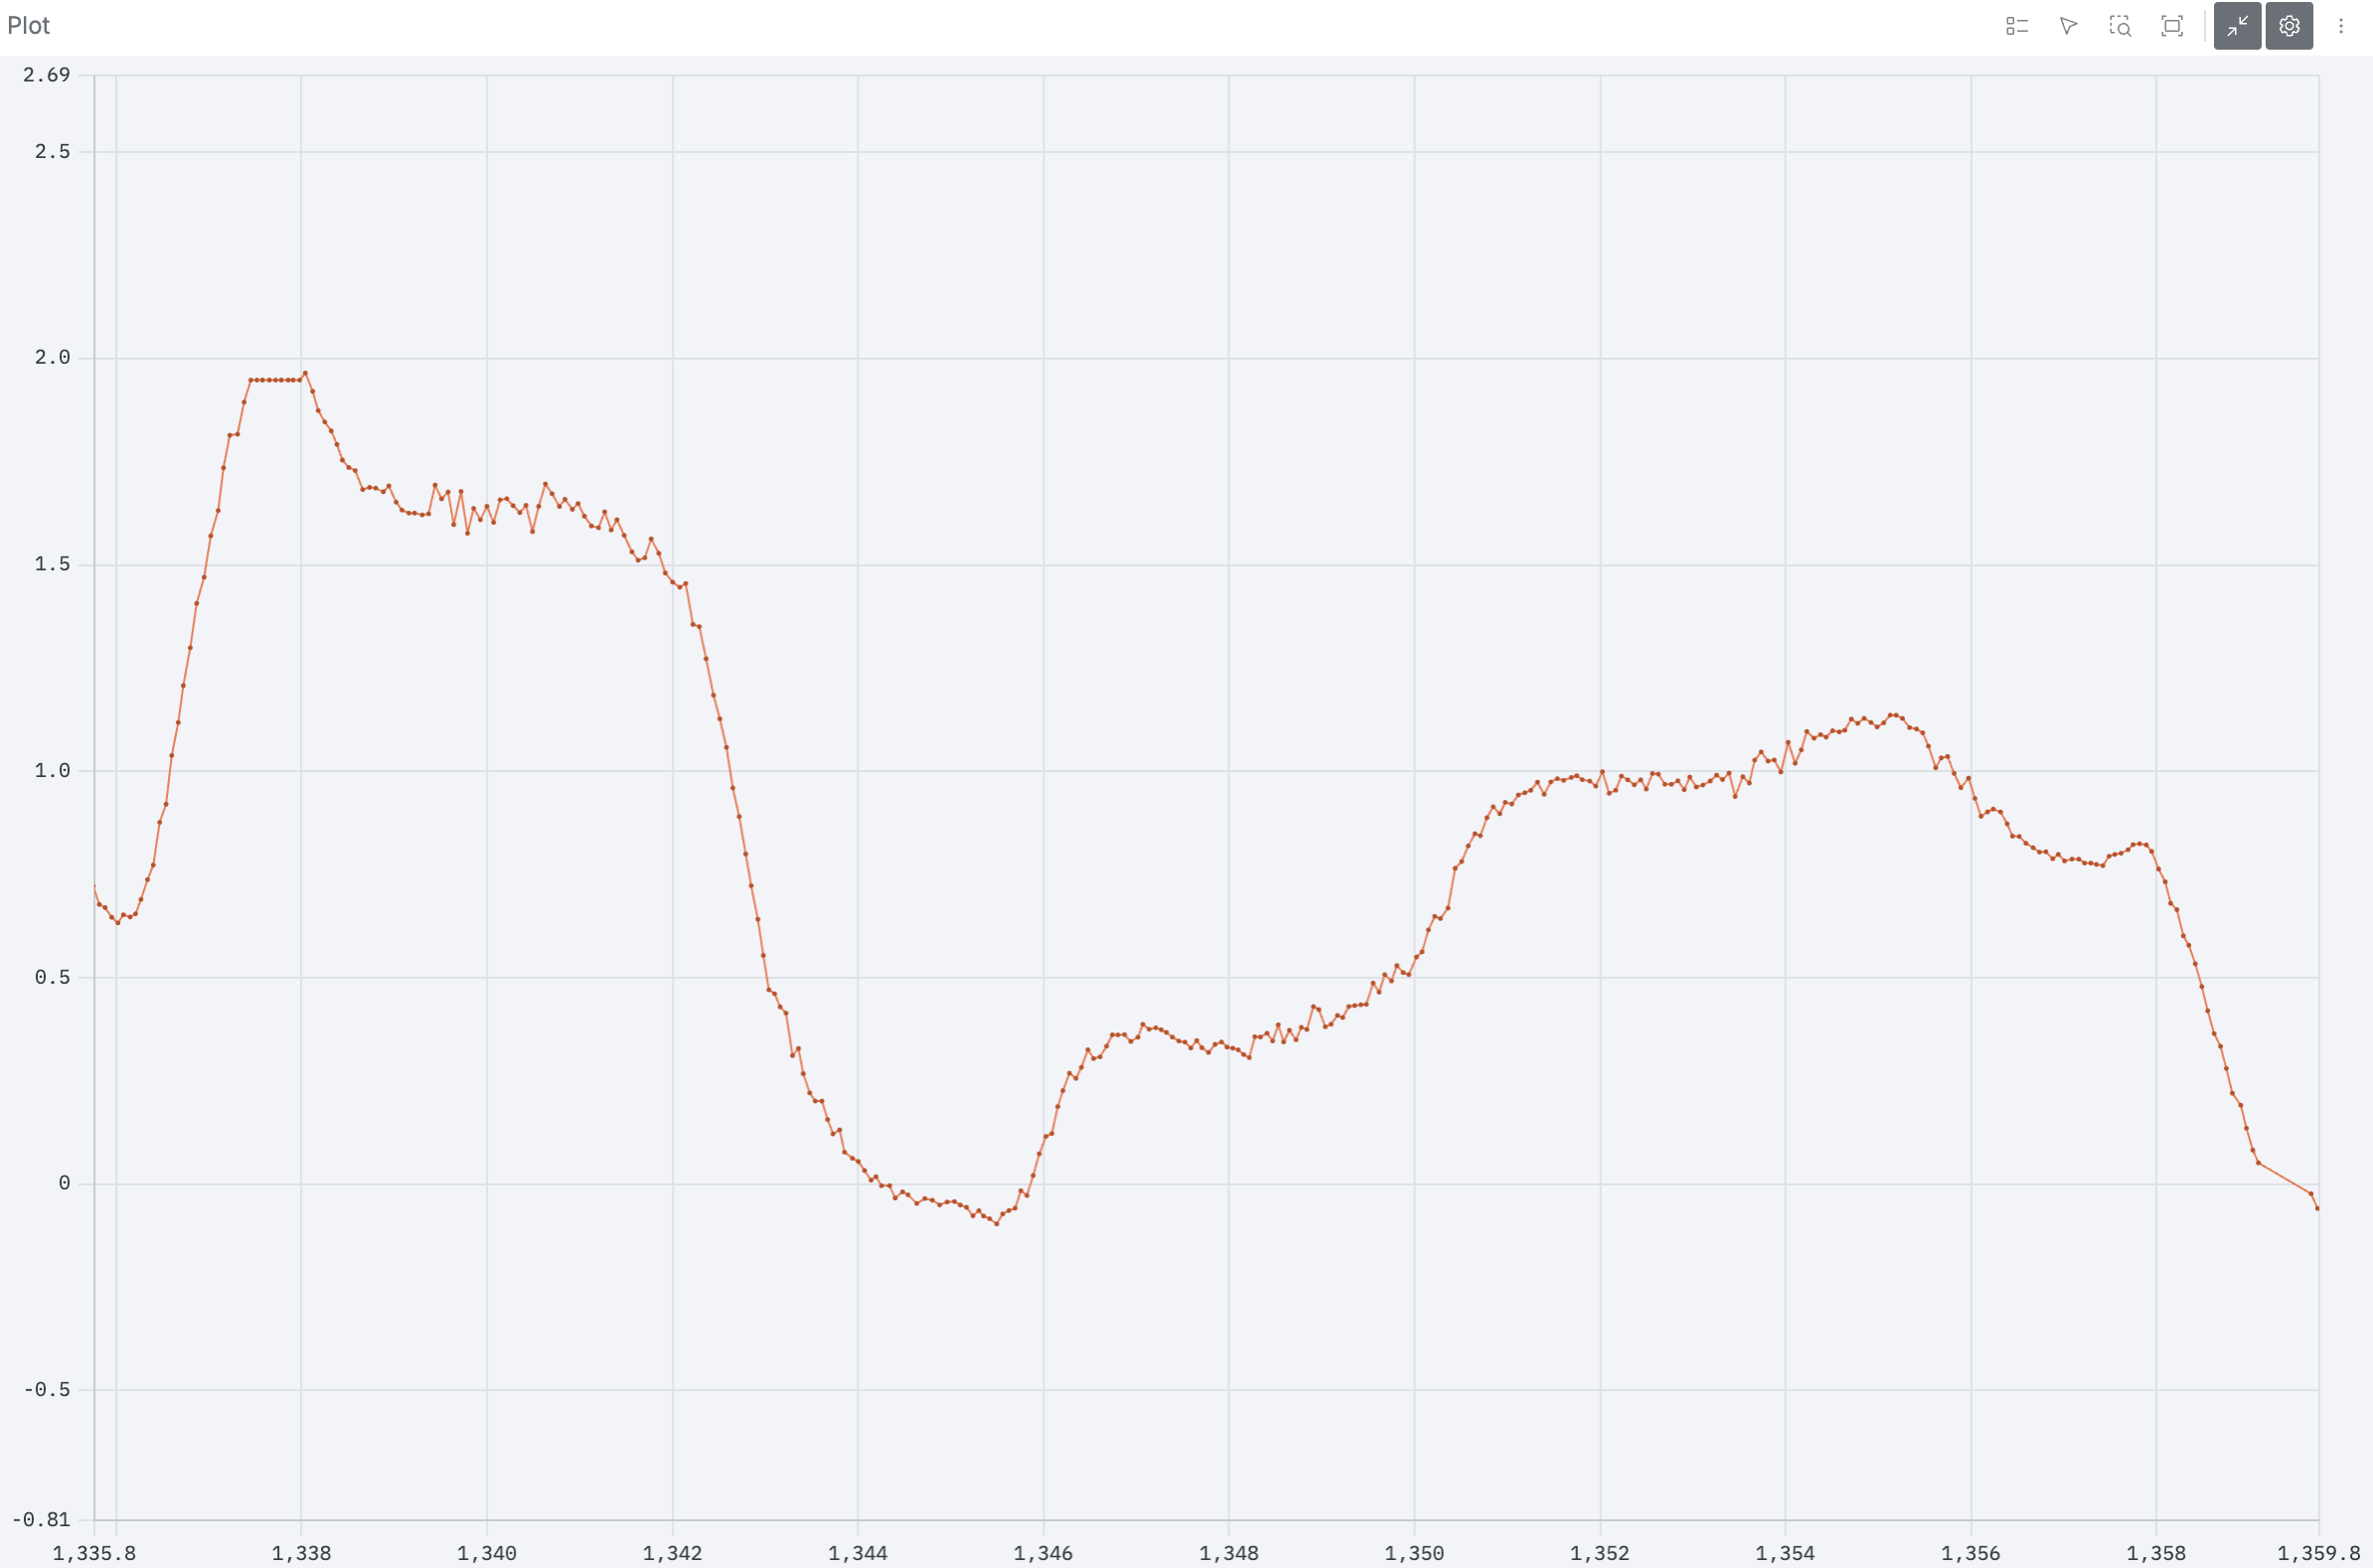
\includegraphics[width=\textwidth, trim={0 0 0 0}, clip]{immagini/log_non_distorto.png}
		\caption{Log con camera global shutter.}
		\label{fig:log_global_shutter}
	\end{subfigure}
	\caption{Due esempi di log del valore di localizzazione X calcolato utilizzando una camera rolling e global shutter. Si nota subito come nella immagine a il valore subisca dei salti improvvisi, mentre nell'immagine b non sono presenti}
	\label{fig:log_rolling_global}
\end{figure}
Utilizzare una camera global shutter risolve completamente il problema, ma al netto di un costo economico maggiore. La camera scelta è basata sul sensore OV7251\footnote{\url{https://www.ovt.com/products/ov7251/}}: ha una risoluzione di 640x480 pixel, bianco e nero e ha un sensore global shutter.

\subsubsection{Parametri della camera in picamera2}
Il modulo Python \texttt{picamera2} permette di configurare la camera a piacere. I parametri scelti per il sistema sono i seguenti:
\begin{itemize}
	\item la configurazione utilizata è la \texttt{create\_video\_configuration}, perché consente di avere un flusso più continuo e costante.
	\item \texttt{size}: permette di impostare la risoluzione dell'immagine, senza tagliarla. Dopo varie prove, è stata scelta una risoluzione di 640×480 per il suo compromesso tra precisione e velocità di elaborazione dell'immagine per la VO.
	\item \texttt{format}: imposta il formato dell'immagine. È stato scelto \texttt{YUV420}, un formato molto leggero e comodo per estrarre l'immagine in bianco e nero.
	\item \texttt{buffer\_count}: impostato ad 1 per avere sempre l'ultima immagine catturata. In questo modo, il tempo tra la richiesta dell'immagine e la risposta resta costante.
	\item \texttt{ExposureTime}: rappresenta il tempo di esposizione del sensore alla luce. Impostando un valore troppo alto, l'immagine risulta troppo chiara e mossa; troppo basso, diventa scura e con delle imperfezioni, dovute dalla compensazione con l'aumento della sensibilità del sensore. Sono stati fatti dei test nell'ambiente in cui il sistema lavora ed è stato scelto un valore di 1500\(\mu s\).
	\item \texttt{FrameDurationLimits}: imposta un limite minimo e massimo dell'intervallo temporale tra un frame e un'altro, quindi imposta il frame rate della camera. È stato impostato a 16666\(\mu s\) sia per il minimo che per il massimo.
\end{itemize}

\subsubsection{Calibrazione della camera}
La calibrazione della camera è un passaggio fondamentale per poter ottenere stime affidabili di posizione e posa del drone attraverso le immagini. Questo procedimento ci permette di ottenere due parametri principali:
\begin{itemize}
	\item Parametri intrinsechi: sono le caratteristiche interne e quelle geometriche del sensore e dell'ottica. Viene rappresentata attraverso una matrice 3x3 composta in questo modo: 
	\[
	\mathbf{K} = \begin{bmatrix} 
		f_x & 0 & c_x \\ 
		0 & f_y & c_y \\ 
		0 & 0 & 1 
	\end{bmatrix}
	\]
	Dove $f_x, f_y$ rappresentano la lunghezza focale della camera in pixel e $c_x, c_y$ sono le coordinate in pixel del centro ottico.
	\item Coefficienti di distorsione: sono dei parametri che rappresentano la distorsione radiale e tangenziale della camera, ovvero descrivono in che modo un obiettivo deforma i raggi luminosi, facendo apparire curve le linee rette. Il numero di questi parametri varia in base alla complessità dell'obiettivo e al modello matematico scelto.
\end{itemize}
Il metodo scelto per la calibrazione della camera è attraverso il modulo OpenCV. Per prima cosa, bisogna scattare delle foto da varie angolazioni di una scacchiera bianco nera, come quella in Fig. \ref{fig:calibration_chess}. Dopodiché, un programma analizzerà tutte le foto scattate e ne restituirà i parametri. È disponibile un esempio sul sito ufficiale di OpenCV \footnote{\url{https://docs.opencv.org/4.13.0/dc/dbb/tutorial_py_calibration.html}}.

\begin{figure}[!htbp]
	\centering
	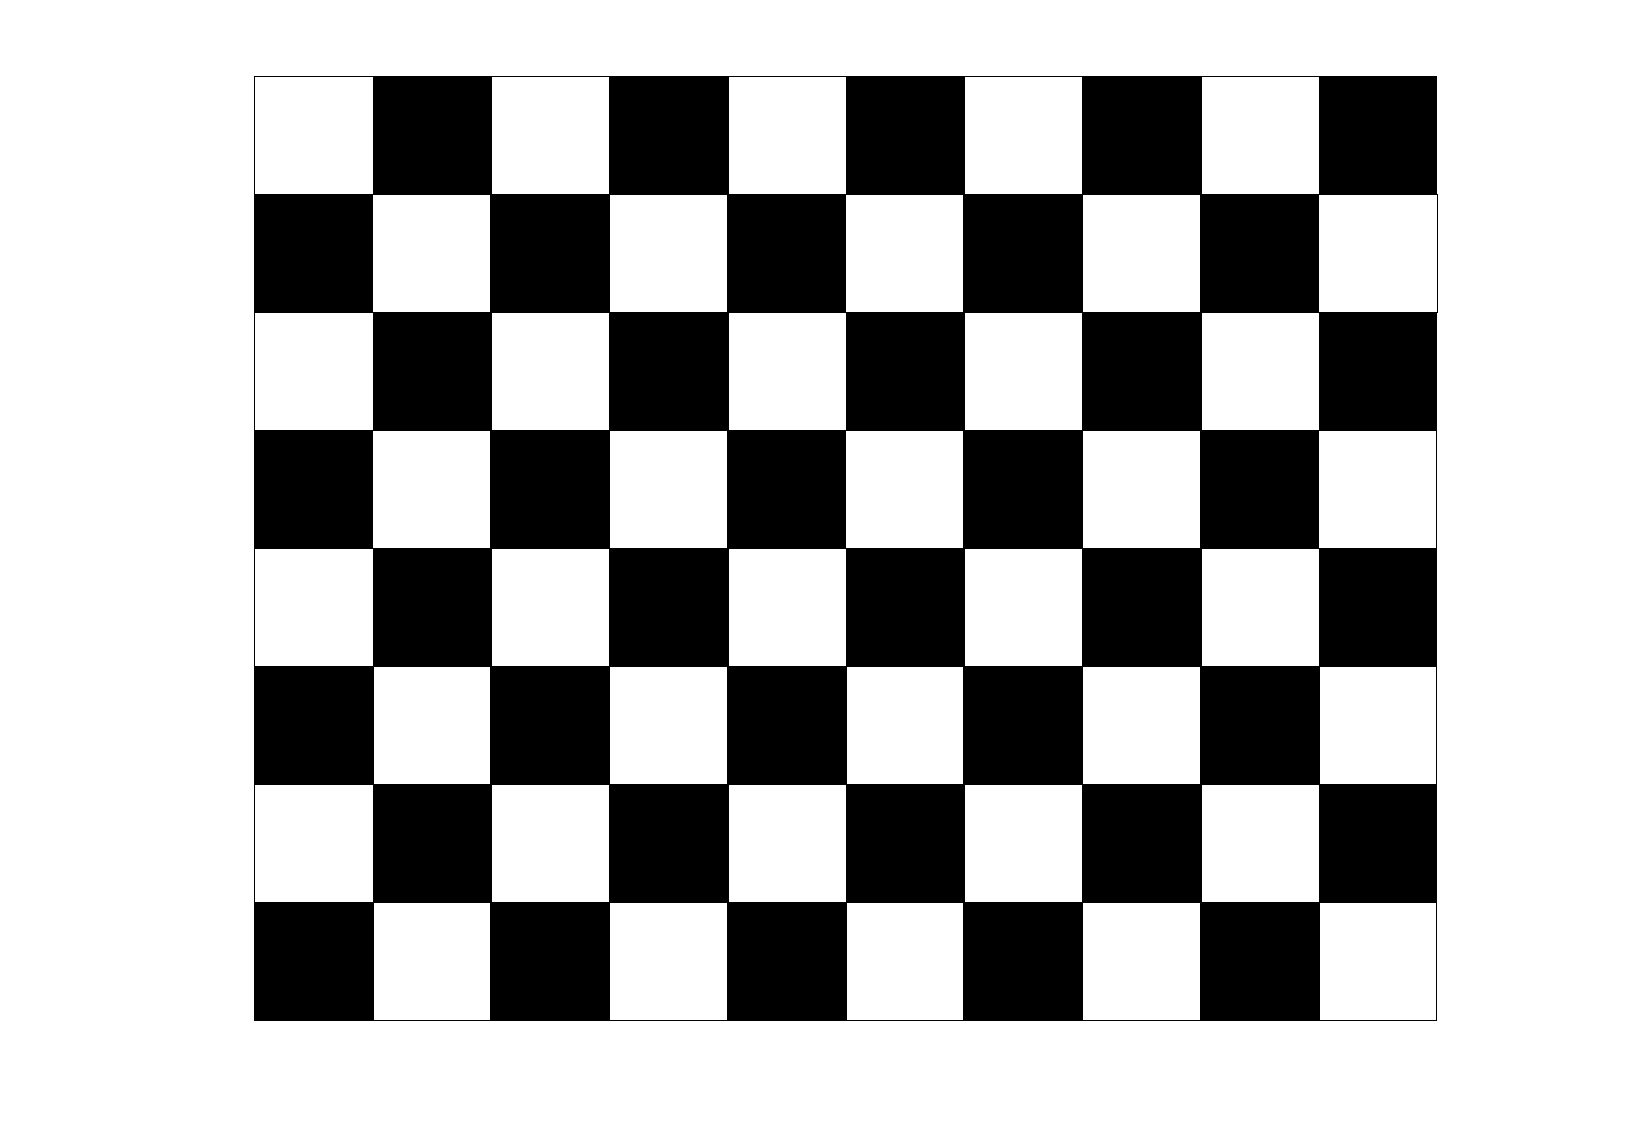
\includegraphics[width = 1\textwidth, trim={0 0 0 0}, clip]{immagini/chessboard-to-print.pdf}
	\caption{Scacchiera 7x9 usata per calibrare una camera. Il tipo di scacchiera viene calcolato contando gli angoli interni, non i quadrati.}
	\label{fig:calibration_chess}
\end{figure}

%   CAPITOLO 4: 
\chapter{Prove sperimentali}
\label{chap:prove_sperimentali}
Nei precedenti capitoli è stata presentata l'architettura e il funzionamento del sistema. In questo capitolo vengono analizzati i test del funzionamento del sistema, eseguiti prima sul simulatore e successivamente su un drone reale.

\section{Esperimenti nell'ambiente di simulazione}
La simulazione è uno strumento molto importante nello sviluppo e nell'implementazione di sistemi nel campo della robotica, poiché consente di effettuare esperimenti in un ambiente non reale, controllato e potenzialmente infinite volte, senza costi dovuti al danneggiamento del sistema.
 In particolare, è stato ampiamente utilizzato per verificare il corretto funzionamento dell'algoritmo per la VO e per la missione, prima di fare i test sul drone reale; inoltre, è stato molto utile per comprendere a fondo il firmware PX4 e tutte le sue meccaniche di volo. \\
 
 \subsection{Architettura del sistema}
 L'ambiente simulato è organizzato in tre componenti principali: a simulazione dell'ambiente (World simulation), la simulazione del drone (Drone simulation) e la simulazione della camera a bordo di esso (Onboard camera simulation).
 
 \paragraph{World simulation} Rappresenta l'ambiente nel quale il drone svolge le sue missioni, rispettando il più fedelmente possibile tutte le leggi geometriche e fisiche di un ambiente reale. Inoltre, il mondo simulato avrà al suo interno vari oggetti necessari per l'esperimento, tra cui vari marker ArUco e quattro mura, per simulare lo scenario di un ambiente chiuso. \\
 Il software utilizzato per simulare l'ambiente è Gazebo\footnote{\url{https://gazebosim.org/home}}.
 
 \paragraph{Drone simulation} È il software che si occupa di riprodurre il comportamento reale del drone, simulandone il movimento e le risposte ai comandi. È molto utile per comprendere il funzionamento del firmware PX4 Autopilot, lo stesso che è presente sul flight controller Holybro Pixhawk 6C Mini del drone reale.
  
 \paragraph{Onboard camera simulation} Infine, anche la camera deve essere simulata. In questo caso, essa fa parte di Gazebo. Le immagini vengono prelevate dallo streaming video tramite GStreamer e OpenCV sulla porta UDP 5600 (OpenCV deve essere compilato con il supporto a GStreamer). Le immagini catturate possono essere elaborate dal sistema di visione artificiale utilizzando gli stessi algoritmi della configurazione reale, permettendo dei test più affidabili.
\subsubsection{Parametri}
Il firmware PX4 Autopilot permette di configurare il comportamento del drone, modificandone i suoi parametri\footnote{\url{https://docs.px4.io/main/en/advanced_config/parameter_reference}}. Durante gli esperimenti, sono stati cambiati alcuni di questi parametri dal loro valore di default, per adattarli alle necessità del sistema. In particolare, sono stati modificati i valori relativi al GPS, VO, filtro di Kalman e quelli relativi al movimento. Ecco la lista dei parametri modificati più importanti:
\begin{itemize}
	\item EKF2\_EV\_DELAY = 20.0 ms
	\item EKF2\_EV\_CTRL = 11 (horizontal position, vertical position, yaw) $\rightarrow$ abilità la VO
	\item EKF2\_GPS\_CHECK = 0
	\item EKF2\_GPS\_CTRL = 0
	\item SIM\_GPS\_USED = 0
	\item SYS\_HAS\_GPS = Disable
	\item EKF2\_HGT\_REF = Vision
	\item MPC\_Z\_P = 1.50 $\rightarrow$ è stato aumentato per far alzare il drone con più decisione. La parte di takeoff è una parte critica del volo, dato che il sistema non riesce a vedere marker per un periodo di tempo e rischia di derivare verso una direzione, il che porta a molte problematiche. Facendo alzare il drone con più decisione questo problema viene ampiamente ridotto.
	\item SDLOG\_PROFILE = 131 $\rightarrow$ permette di definire cosa vedere nei file di log.
\end{itemize} 
Un parte fondamentale che merita un approfondimento è come viene calcolato il parametro EKF2\_EV\_DELAY\footnote{\url{https://docs.px4.io/main/en/ros/external_position_estimation\#tuning-EKF2_EV_DELAY}}. Esso corrisponde alla differenza di tempo (in millisecondi) tra la stima della VO e quella dell'IMU, e si può trovare osservando i log. Ad esempio, in Fig. \ref{fig:sim_ev_delay} è rappresentata dalla freccia rossa, e corrisponde a circa 20ms.

\begin{figure}[!htbp]
	\centering
	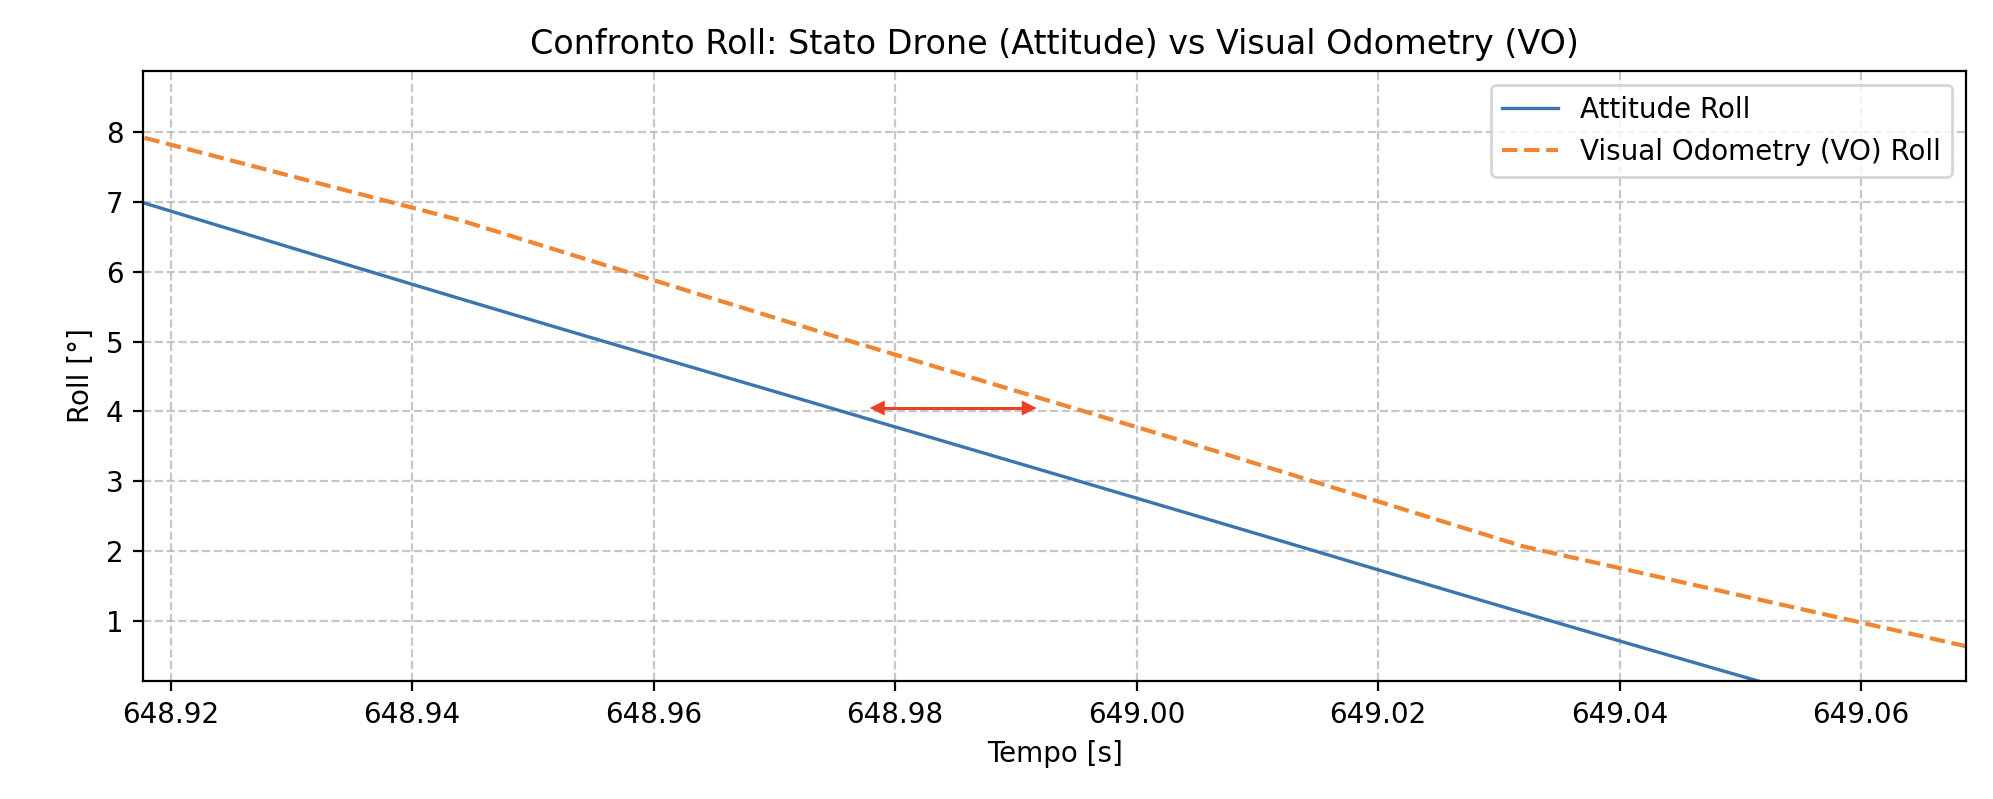
\includegraphics[width = 1\textwidth, trim={0 0 0 0}, clip]{immagini/sim_ev_delay.png}
	\caption{Grafico log del simulatore che confronta il roll della VO e quello dell'IMU per il calcolo del parametro EKF2\_EV\_DELAY.}
	\label{fig:sim_ev_delay}
\end{figure}

\subsubsection{Ambiente}
Il mondo simulato comprende uno scenario contenente 16 marker diversi recintati da dei muri (Fig. \ref{fig:gazebo}). I marker hanno una grandezza di mezzo metro, e sono distanti 2 metri l'uno dall'altro. La distanza e la grandezza dei marker è stata valutata in base al FOV (Field of View) della camera e al tipo di missione da svolgere.\\
La tipologia di drone scelto per l'ambiene simulato è il modello \texttt{gz\_x500\_mono\_cam\_down}\footnote{\href{https://docs.px4.io/main/en/sim_gazebo_gz/vehicles\#x500-quadrotor-with-monocular-camera-down-facing}{\texttt{https://docs.px4.io/main/en/sim\_gazebo\_gz/vehicles\#x500-quadrotor-with-monocular-}\\ \texttt{camera-down-facing}}}. \\
La descrizione json della configurazione dei marker è presente sul github del progetto nel file \path{src/marker_info/aruco_floor_sim.json}; mentre la descrizione del mondo è disponibile nel file \path{my_worlds/aruco_floor.sdf}.
 \begin{figure}[!htbp]
	\centering
	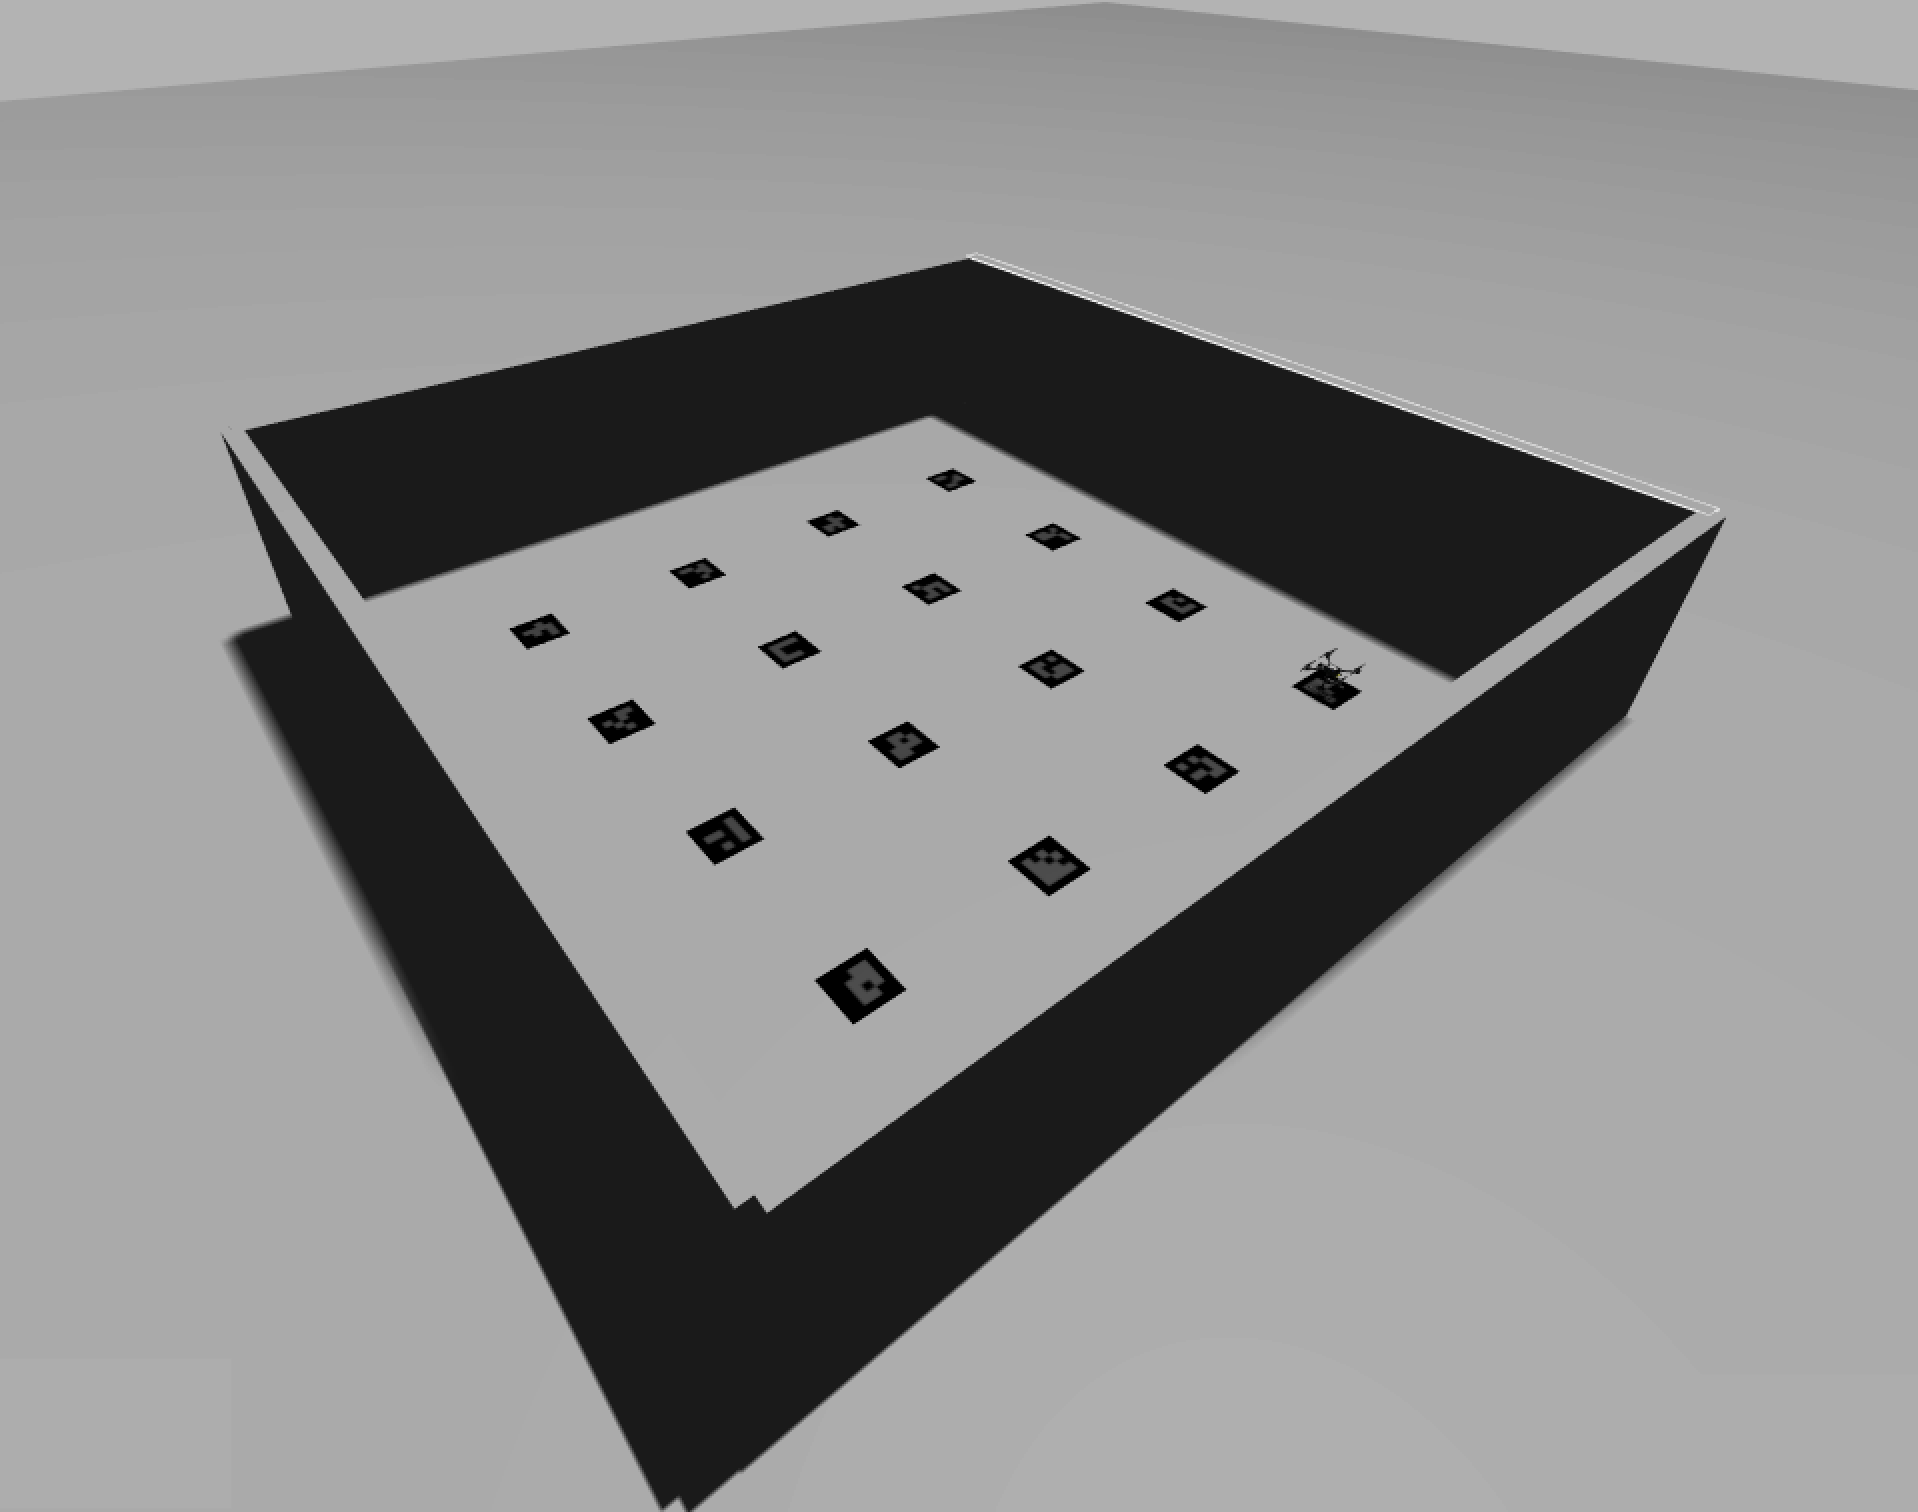
\includegraphics[width=0.7\textwidth, trim={0 0 0 0}, clip]{immagini/gazebo.png}
	\caption{Screenshot del mondo creato dentro Gazebo.}
	\label{fig:gazebo}
\end{figure}

\subsection{Presentazione e analisi dei risultati}
In questa sezione vengono presentati e analizzati i risultati dei test effettuati nell'ambiente simulato. \\
L'analisi si basa principalmente sui file di log che vengono registrati ad ogni sessione di volo. Essi contengono le informazioni relative allo stato del drone, le stime di posizione e posa e i dati che il sistema riceve dalla VO. \\ \\
La missione eseguita e registrata dal log presentata in questa sezione consiste nel raggiungere la posizione NED (4, 2, -1.4) in modalità hoverpoint, partendo dalla (0, 0, -1.4); successivamente, il drone esegue due cerchi grazie alla modalità waypoint; infine, il veivolo ritorna al punto di partenza e atterra. \\ \\
Il log della traiettoria della missione eseguita dal drone è visibile nelle Fig. \ref{fig:sim_xy}, \ref{fig:sim_z}. La traiettoria arancione indica le informazioni inviate al flight controller grazie alla VO; mentre quella blu rappresenta lo stato del filtro di Kalman dopo la fusione dei dati. \\
 \begin{figure}[!htbp]
	\centering
	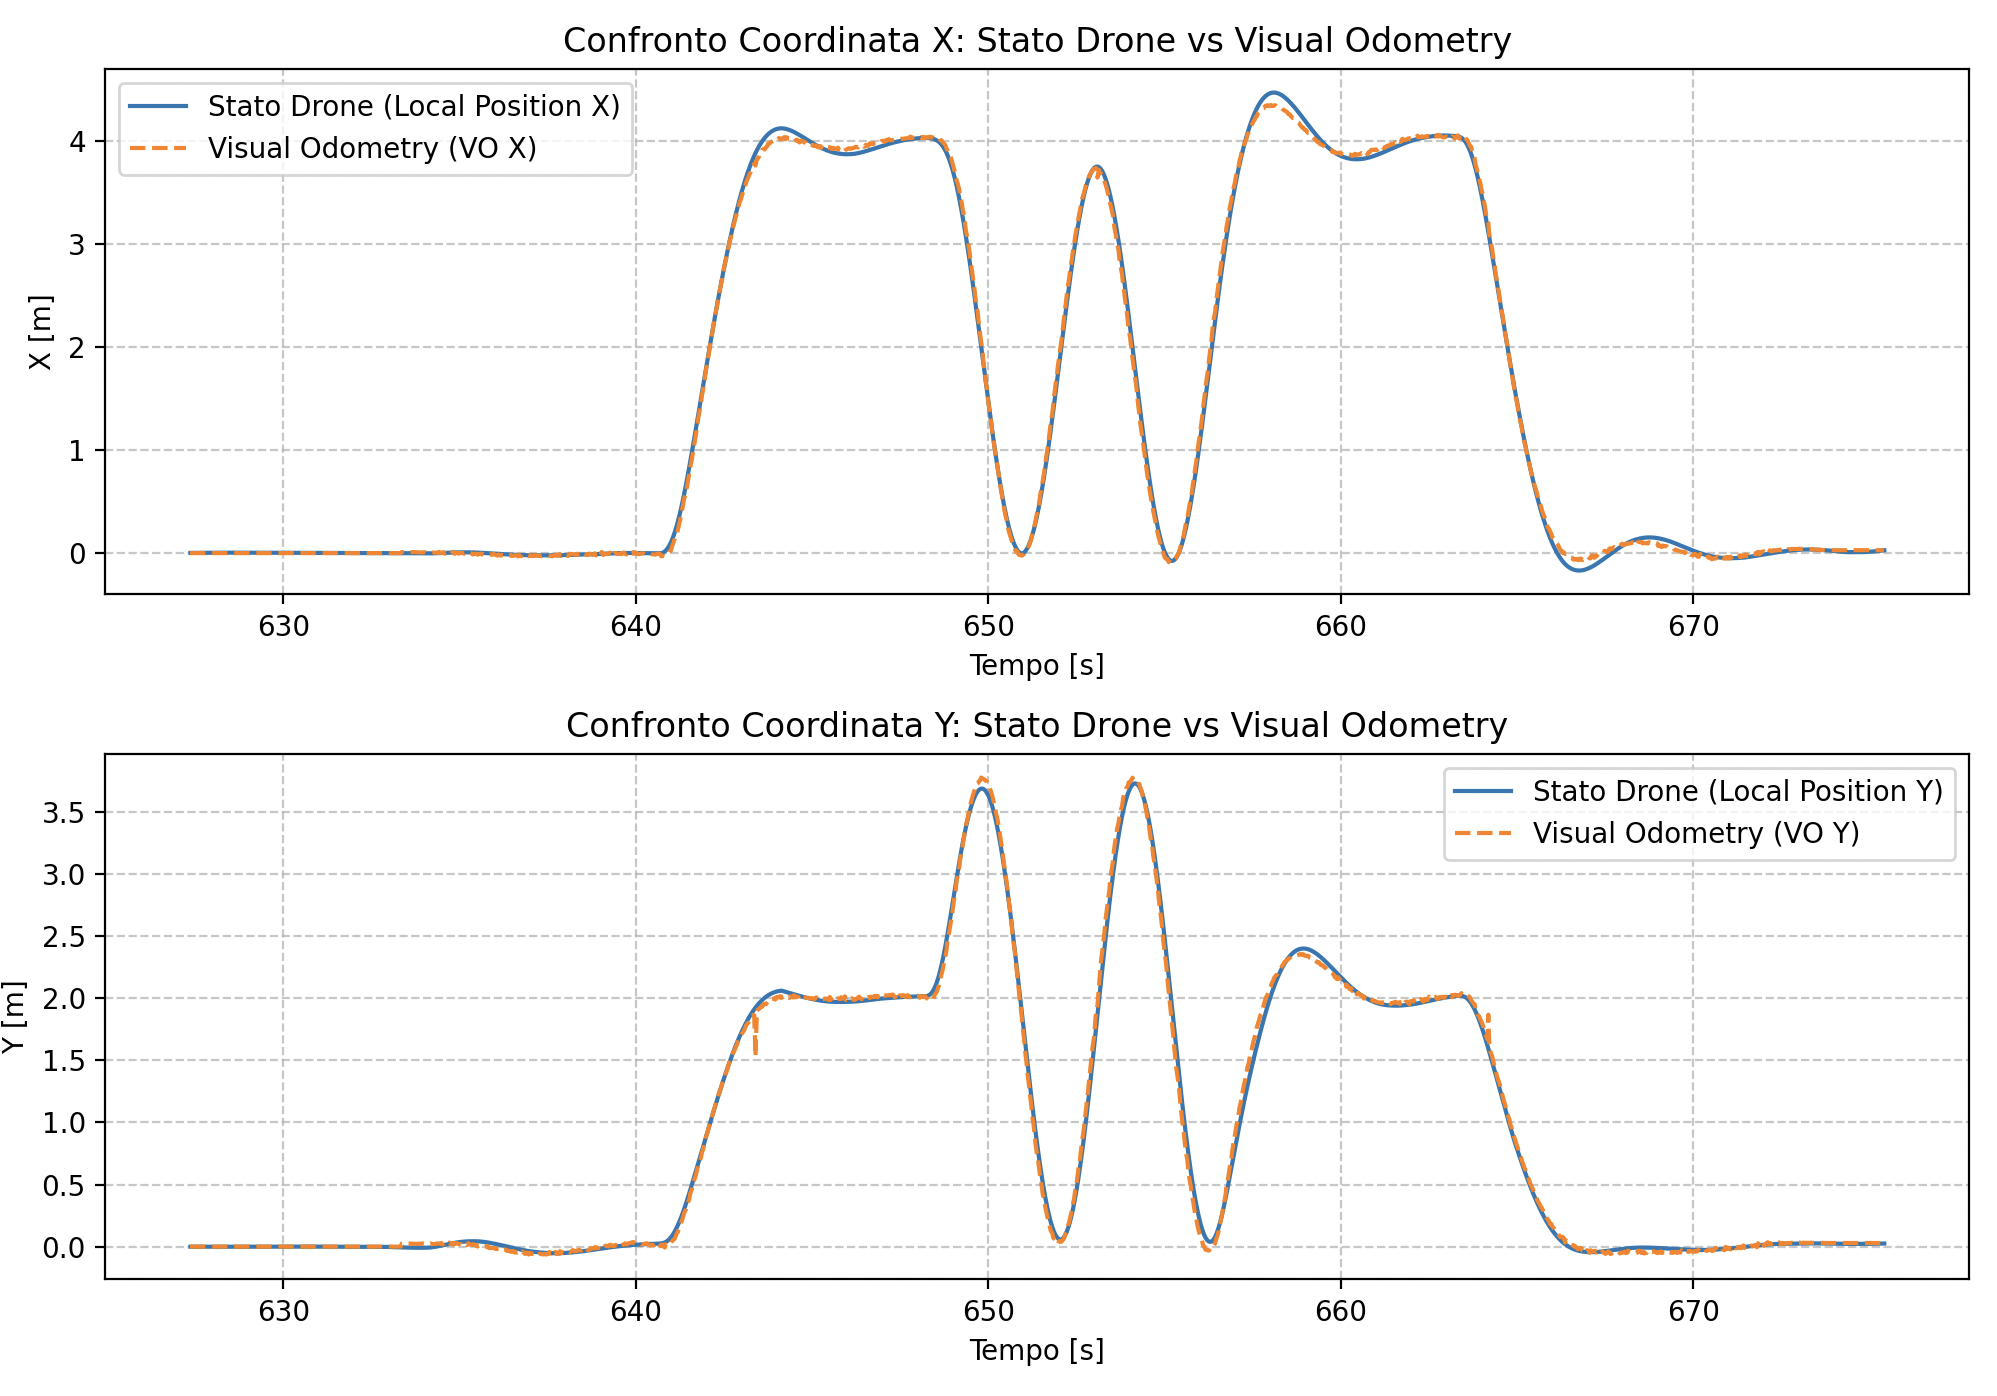
\includegraphics[width=1\textwidth, trim={0 0 0 0}, clip]{immagini/sim_xy.png}
	\caption{Grafico log del simulatore che confronta le coordinate XY della VO e lo stato nel filtro di Kalman.}
	\label{fig:sim_xy}
\end{figure}
 \begin{figure}[!htbp]
	\centering
	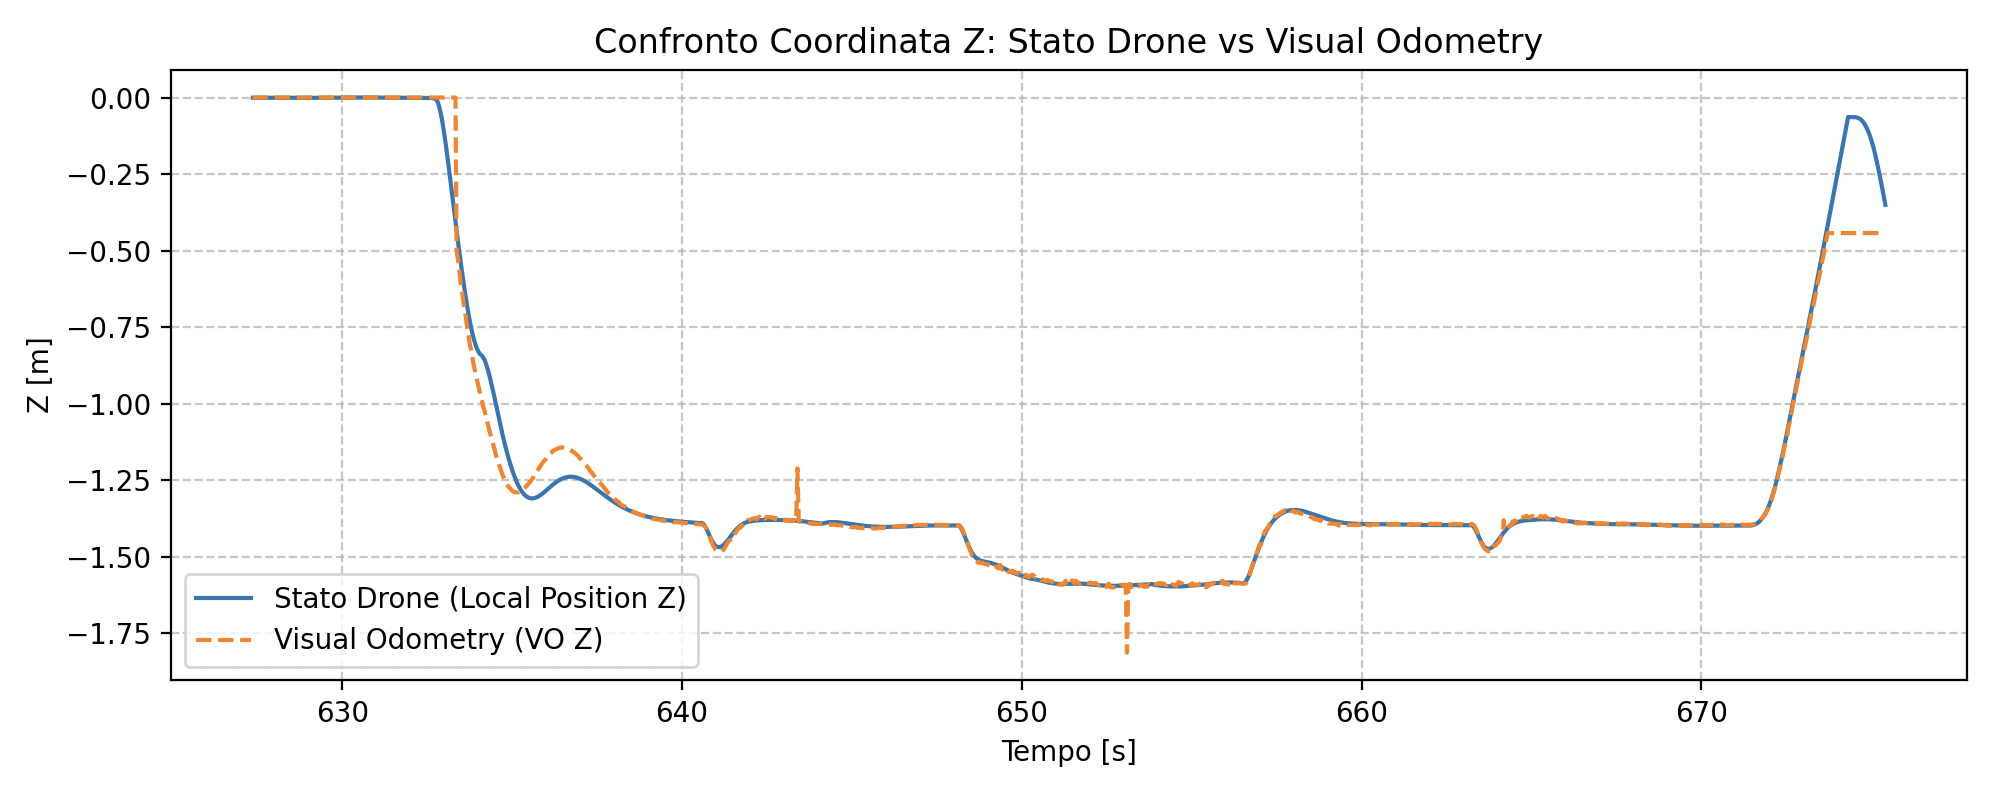
\includegraphics[width=1\textwidth, trim={0 0 0 0}, clip]{immagini/sim_z.png}
	\caption{Grafico log del simulatore che confronta la coordinata Z della VO e lo stato nel filtro di Kalman.}
	\label{fig:sim_z}
\end{figure} \\
Possiamo subito notare come lo stato del filtro di Kalman segua quello della VO, ma non è uguale; questo perchè fa una fusione tra tutti dati, non solo della VO. Inoltre, si può osservare che anche se la VO ha un discostamento anomalo (nelle varie figure se ne possono vedere un paio), il filtro di Kalman corregge questo difetto. \\ 
Per quanto riguarda l'asse Z, possiamo osservare il momento del decollo e di atterraggio. La cosa particolare di queste operazioni è il momento in cui il drone inizia a vedere (o non vede più, in caso di atterraggio) i marker; ma soprattutto anche qui si vede bene il lavoro del filtro di Kalman: nella fase di atterraggio, quando non vede più il marker, di può osservare come la coordinata Z dello stato del drone continua a tendere verso terra; questo avviene grazie alla fusione dei dati con l'IMU. \\
Come spiegato nella Sez. \ref{sec:problema:localizzazione:kalman}, l'IMU anche se correttamente calibrato ha un problema di drift, e qui lo si può notare dal fatto che la coordinata Z non arrivi a 0.\\
Un'ultima considerazione che si può fare è riguardo all'innalzamento dell'altezza del drone, visibile in Fig. \ref{fig:sim_z}: si verificano durante gli spostamenti e una possibile ipotesi di questo effetto è che accade a causa del cambio d'assetto. \\ \\
I log generati dal flight controller non contengono direttamente gli angoli roll, pitch e yaw, ma salvano i quaternioni. Per osservare al meglio i risultati, le Fig. \ref{fig:sim_roll}, \ref{fig:sim_pitch}, \ref{fig:sim_yaw} rappresentano gli angoli convertiti a partire dai quaternioni nel log.\\
Per quanto riguarda i grafici di roll (Fig. \ref{fig:sim_roll}) e pitch (Fig. \ref{fig:sim_pitch}), possiamo notare che i dati della VO e quelli dell'IMU sono praticamente uguali. 
\begin{figure}[!htbp]
	\centering
	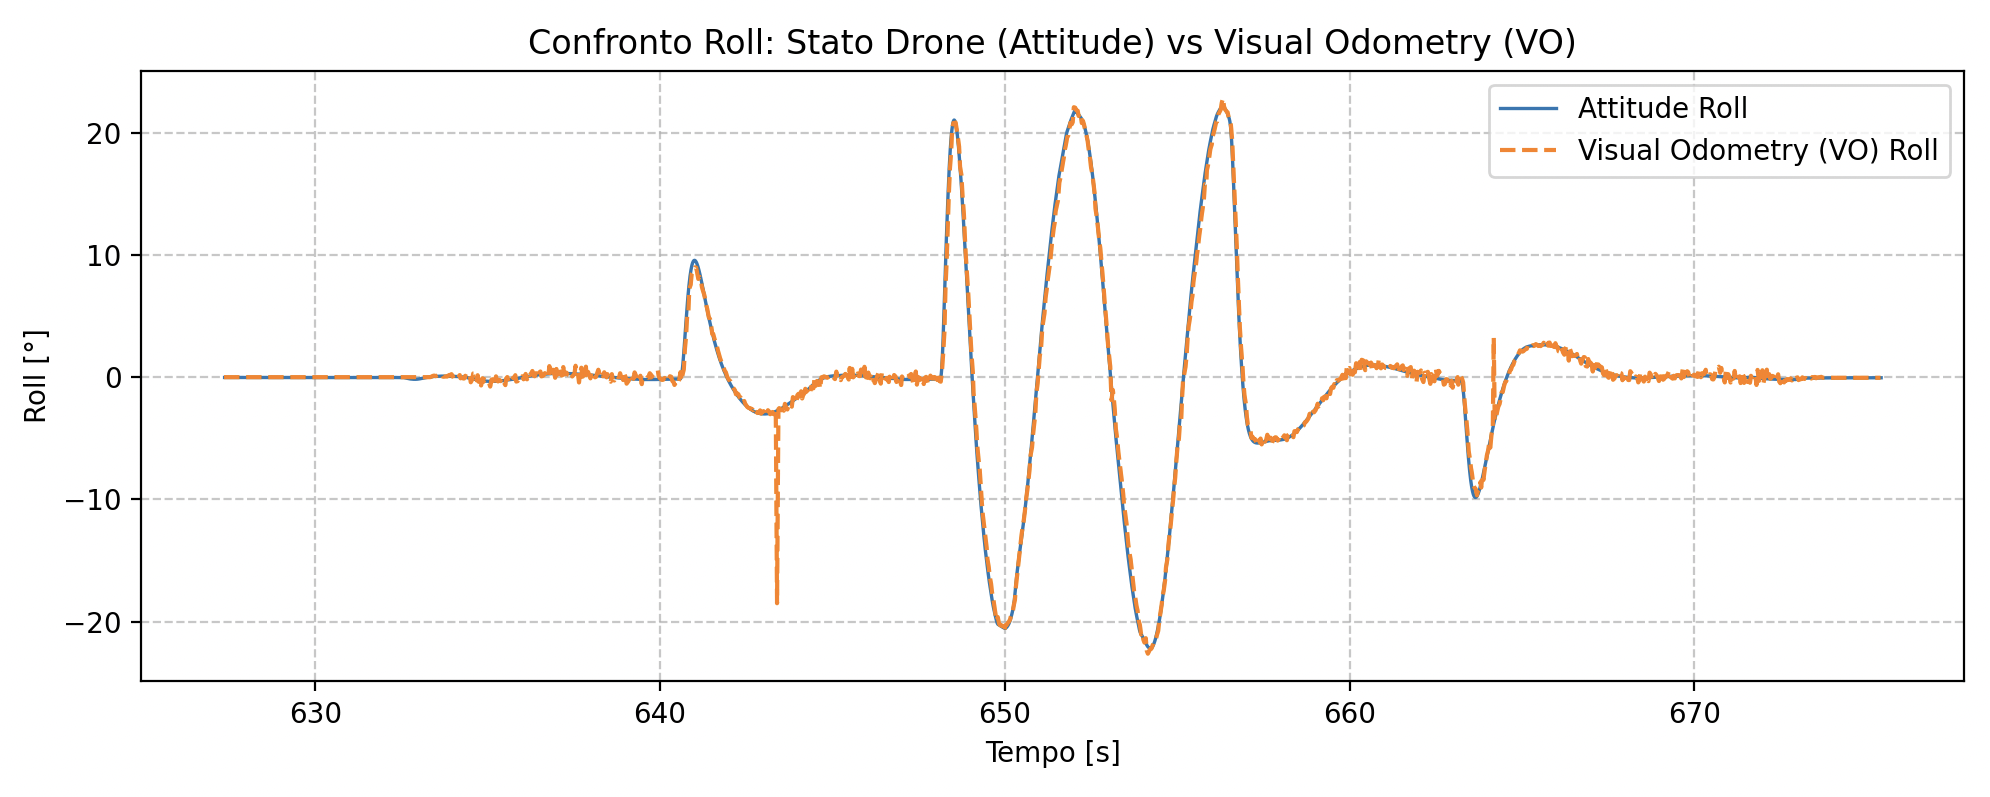
\includegraphics[width = 1\textwidth, trim={0 0 0 0}, clip]{immagini/sim_roll.png}
	\caption{Grafico log del simulatore che confronta il roll della VO e quello dell'IMU.}
	\label{fig:sim_roll}
\end{figure}
\begin{figure}[!htbp]
	\centering
	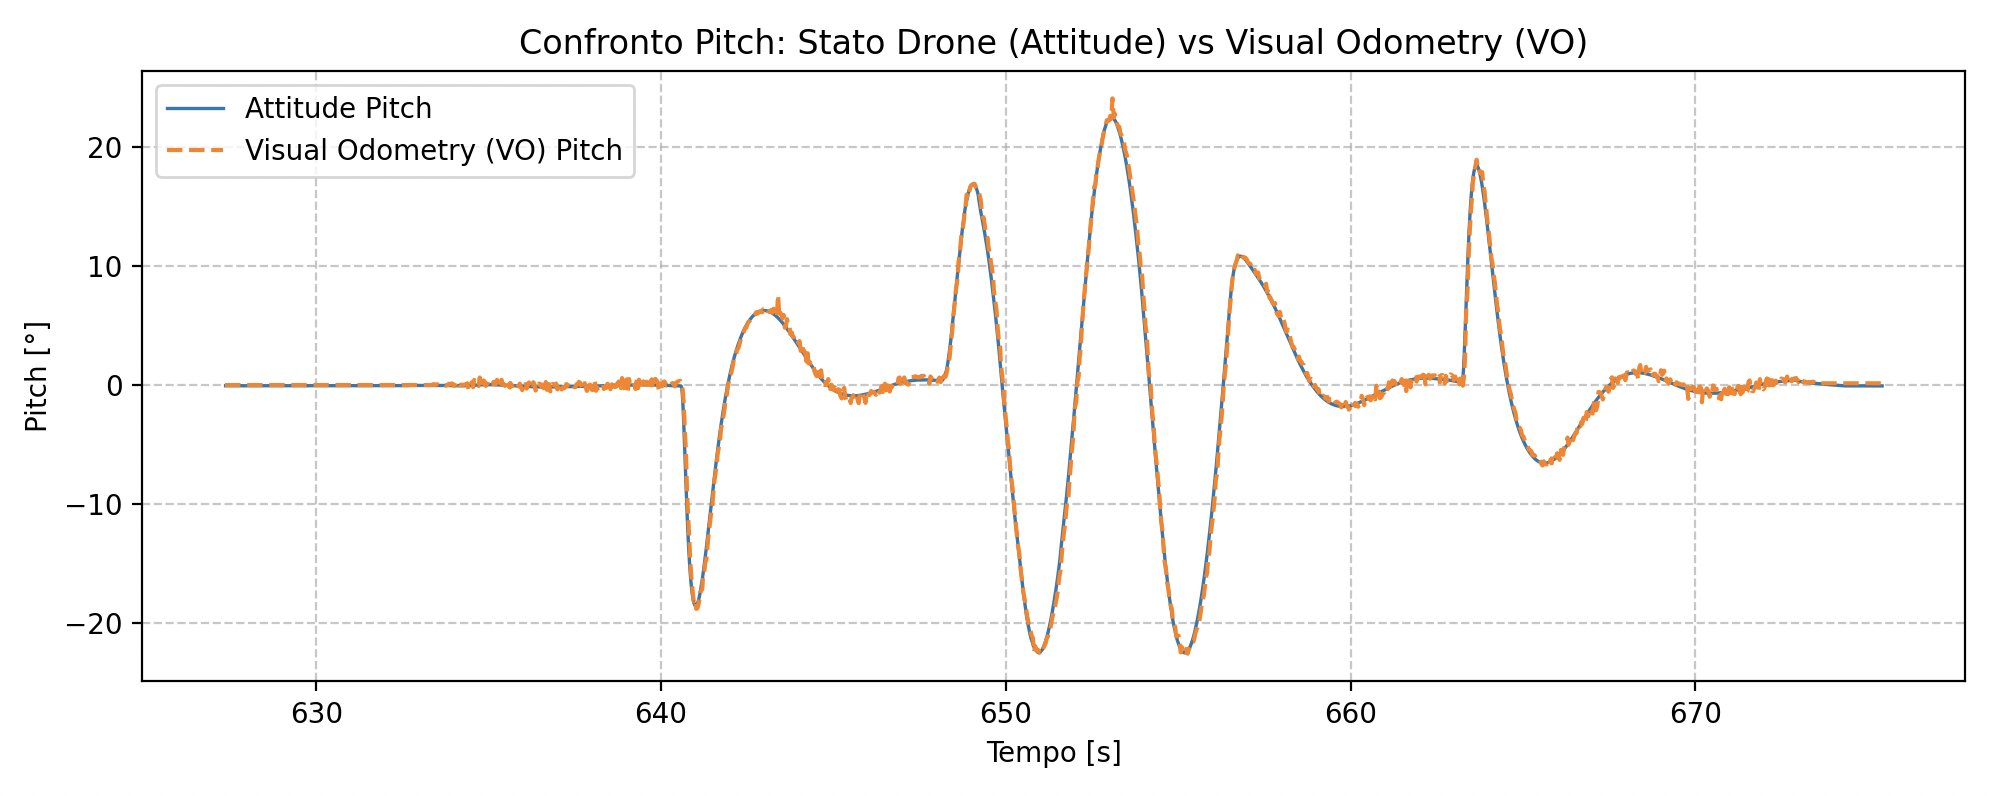
\includegraphics[width = 1\textwidth, trim={0 0 0 0}, clip]{immagini/sim_pitch.png}
	\caption{Grafico log del simulatore che confronta il pitch della VO e quello dell'IMU.}
	\label{fig:sim_pitch}
\end{figure} \\
Un'osservazione importante da fare è che nei grafici si possono osservare delle fluttuazioni rapide, soprattutto quando gli angoli solo vicino allo zero; questo accade perchè risulta molto difficile effettuale il calcolo preciso di questi valori, soprattutto quando la camera di trova perpendicolare al marker. Nonostante ciò, i dati prodotti risultano utilizzabili. \\ \\
I valori dell'angolo yaw generati dalla missione sono osservabili dalla Fig. \ref{fig:sim_yaw}.
\begin{figure}[!htbp]
	\centering
	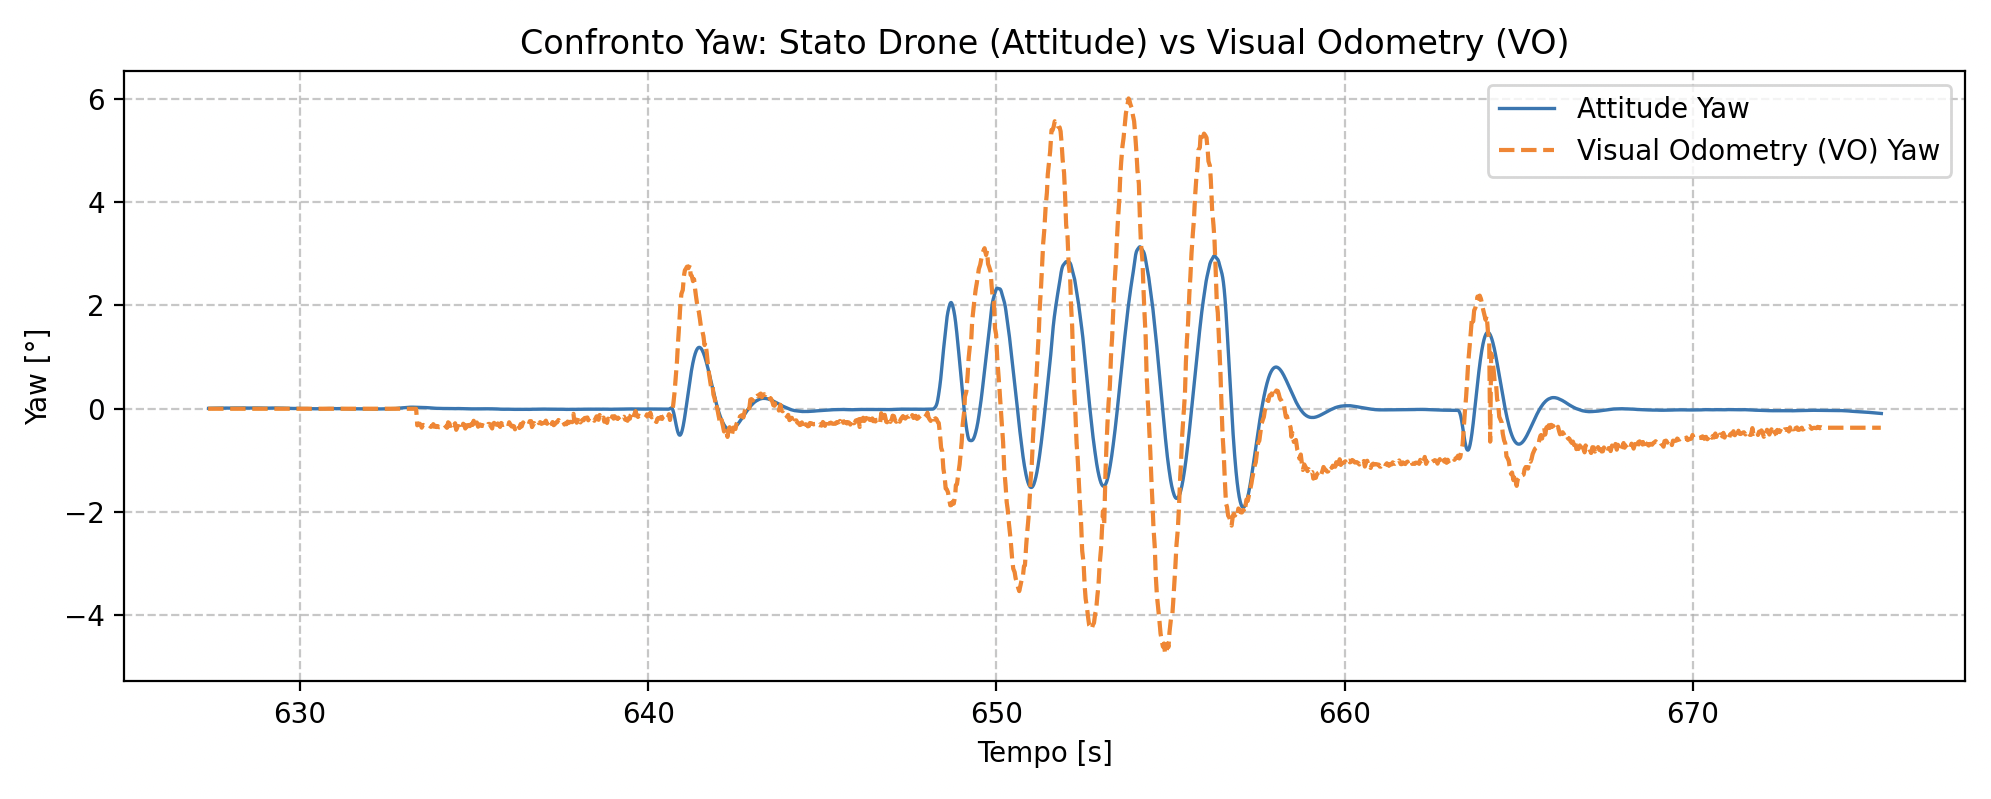
\includegraphics[width = 1\textwidth, trim={0 0 0 0}, clip]{immagini/sim_yaw.png}
	\caption{Grafico log del simulatore che confronta lo yaw della VO e quello dell'IMU.}
	\label{fig:sim_yaw}
\end{figure}\\
Una prima osservazione che possiamo fare è al tempo 634, ovvero al momento in cui il drone inizia a vedere i marker. Anche in questo caso sono presenti le discontinuità notate in precedenza. \\
Si può osservare che sono presenti delle parti in cui i valori dell'IMU non raggiungono la VO. Come nel caso della coordinata Z, questo evento si verifica durante gli spostamenti del drone; quindi, anche in questo caso l'ipotesi è che sia causato dal cambio d'assetto dovuto dallo spostamento del drone. \\ \\
Infine, per quanto riguarda l'esecuzione della missione, il drone è riuscita ad eseguirla senza problemi, volando in modo preciso e deciso, alternando le due modalità di target senza intoppi ed eseguendo le traiettorie dei cerchi in modo accettabile.

\section{Esperimenti di volo reale}
Dopo aver fatto tutte le prove necessarie per costruire il sistema e una volta raggiunto un certo livello di fiducia su di esso, si può passare al test in un ambiente e con un drone reale. In questa sezione vengono descritti ambiente e sistema, seguiti dai risultati ottenuti.

\subsection{Architettura del sistema}
Gli esperimenti con il drone reale sono stati eseguiti utilizzando il sistema hardware presentato nei capitoli precedenti, integrato con i software sviluppati e in parte utilizzati anche negli esperimenti condotti sul simulatore. Rispetto a questi ultimi, il drone fisico introduce ulteriori aspetti legati ai sensori fisici, alle prestazioni del companion computer e all'ambiente.
\subsubsection{Hardware}
Il sistema di volo è costituito da un flight controller Holybro Pixhawk 6C Mini, dotato del firmware PX4 Autopilot, e di un Raspberry Pi 3B, utilizzato come companion computer e incaricato di eseguire i software sviluppati. Quest'ultimo ha installato una camera global shutter OV7251, via connettore CSI del Raspberry; e viene alimentato attraverso un modulo step-down adeguato, che abbassa la tensione dai 14.8V nominali della batteria ai 5V necessari al Raspberry. Per finire, la comunicazione tra flight controller e companion computer avviene via seriale attraverso il protocollo MAVLink 
\subsubsection{Parametri}
Come già visto nel caso del simulatore, anche nel drone reale si devono cambiare alcuni dei parametri di default, per poter utilizzare il sistema correttamente. Qui sono elencati quelli più importanti:
\begin{itemize}
	\item EKF2\_EV\_DELAY = 160.0 ms
	\item EKF2\_EV\_CTRL = 11 (horizontal position, vertical position, yaw) $\rightarrow$ abilità la VO
	\item EKF2\_GPS\_CHECK = 0
	\item EKF2\_GPS\_CTRL = 0
	\item SYS\_HAS\_GPS = Disable
	\item EKF2\_HGT\_REF = Vision
	\item MPC\_Z\_P = 1.50 $\rightarrow$ anche in questo caso è stato aumentato per far alzare il drone con più decisione, e quindi diminuire il difetto di non riuscire a trovare il marker in fase di decollo.
	\item SDLOG\_PROFILE = 1155 $\rightarrow$ permette di definire cosa vedere nei file di log.
\end{itemize} 
Il calcolo del parametro EKF2\_EV\_DELAY è stato eseguito con lo stesso metodo di prima, eseguendo una media dei valori trovati. \\
Infine, a differenza del simulatore, nel drone reale è necessario calibrare tutti i sensori per ottenere dei risultati più precisi, anche più di una volta. Questo accade perchè sensori come l'IMU tendono a scalibrarsi con il passare del tempo e dell'uso.

\subsubsection{Ambiente}
Gli esperimenti sono stati eseguiti dentro un magazzino al chiuso, utilizzando nove marker diversi. I marker hanno una grandezza di 18.5 centimetri, distanti 80 centimetri l'uno dall'altro. Come nel simulatore, anche nel test reale le distanze e la grandezza dei marker sono state scelte in base ai componenti utilizzati nel sistema e al tipo di missione da eseguire. Una foto dell'ambiente è disponibile nella Fig. \ref{fig:magazzino}. \\
La descrizione dei marker è presente nel file \path{src/marker_info/aruco_floor.json}.
\begin{figure}[!htbp]
	\centering
	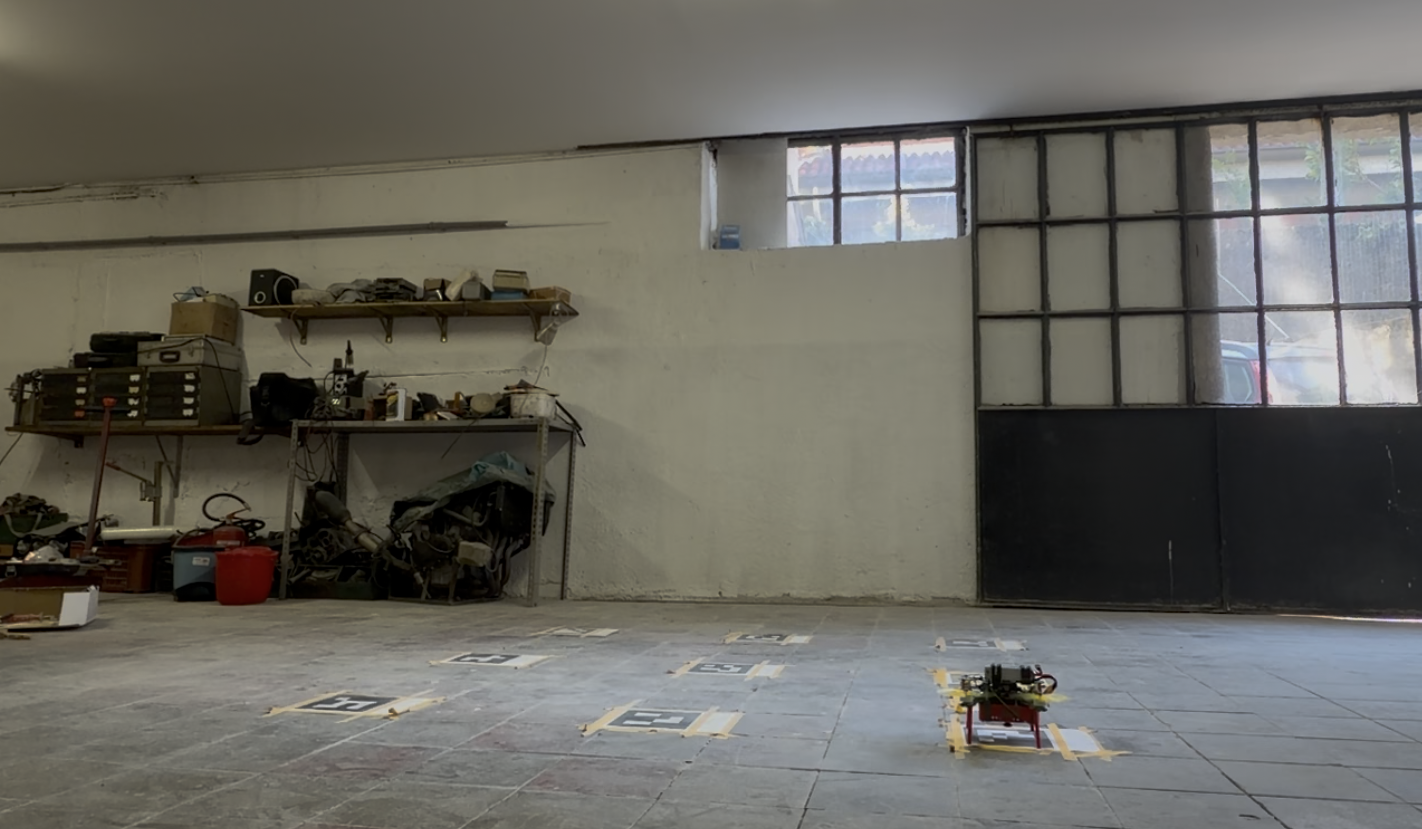
\includegraphics[width = 0.75\textwidth, trim={0 0 0 0}, clip]{immagini/magazzino.png}
	\caption{Foto scattata dentro l'ambiente dove sono stati fatti i test con il drone reale.}
	\label{fig:magazzino}
\end{figure}

\subsection{Presentazione e analisi dei risultati}
In questa sezione vengono presentati i risultati ottenuti durante le prove di volo reale, con l'obiettivo di valutare il funzionamento di tutto il sistema nella realtà dopo le prove fatte al simulatore. \\
L'analisi si basa sul confronto tra la VO inviata dal companion computer e i dati che il flight controller registra\\ \\
Analizziamo i valori di roll e pitch, visualizzabili dalle Fig. \ref{fig:real_roll}, \ref{fig:real_pitch}.
\begin{figure}[!htbp]
	\centering
	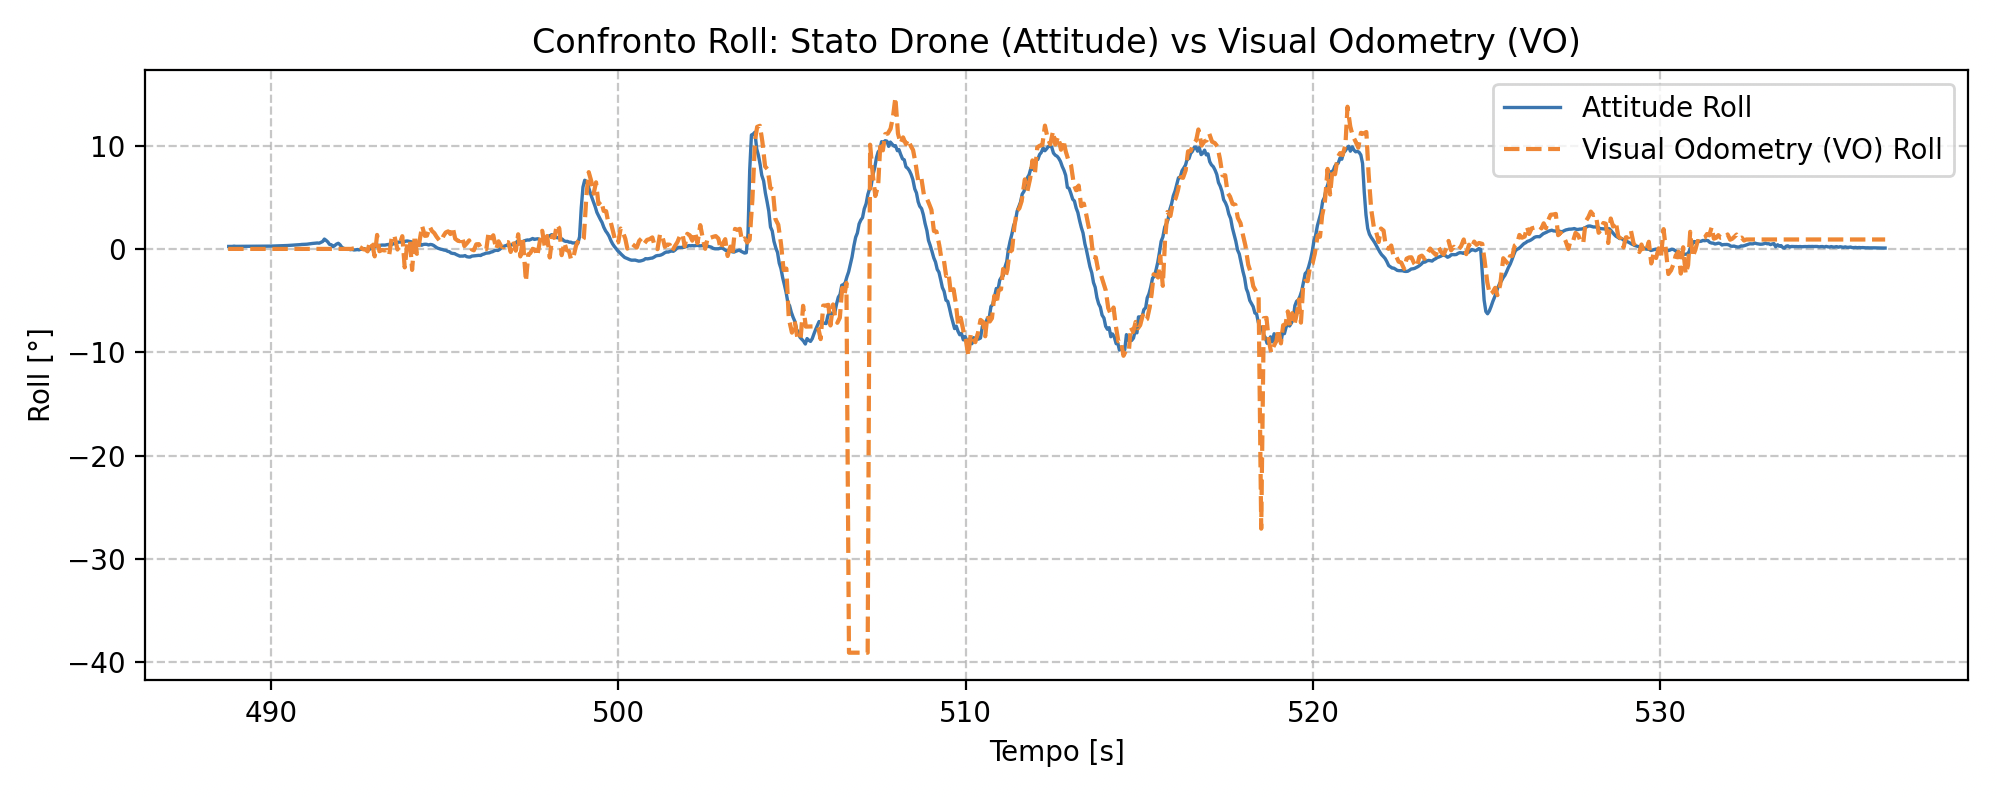
\includegraphics[width = 1\textwidth, trim={0 0 0 0}, clip]{immagini/real_roll.png}
	\caption{Grafico log di volo reale che confronta il roll della VO e quello dell'IMU.}
	\label{fig:real_roll}
\end{figure}
\begin{figure}[!htbp]
	\centering
	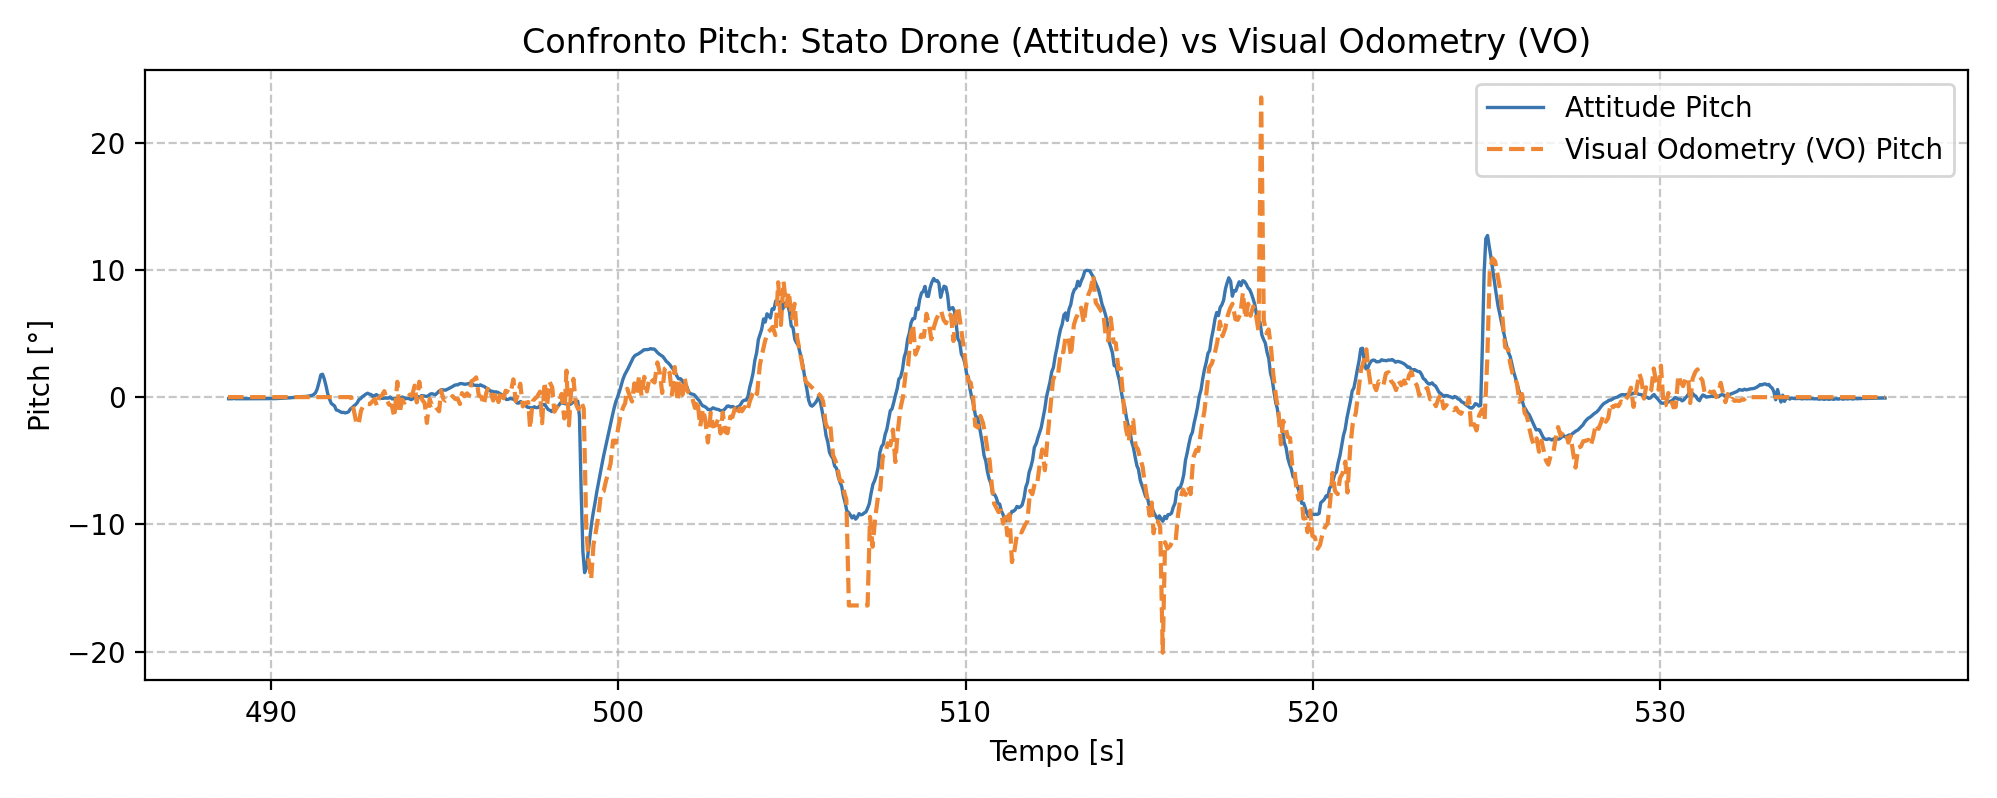
\includegraphics[width = 1\textwidth, trim={0 0 0 0}, clip]{immagini/real_pitch.png}
	\caption{Grafico log di volo reale che confronta il pitch della VO e quello dell'IMU.}
	\label{fig:real_pitch}
\end{figure}
Possiamo osservare che i valori di IMU e VO si inseguono a vicenda; il problema sono le fluttuazioni rapide riscontrate anche nel simulatore. Nel drone reale, queste fluttuazioni sono più accentuate e causano delle instabilità nel volo. Nella Fig. \ref{fig:real_probl} è presente uno zoom del grafico di roll, e si possono notare questa variazioni di circa 2°, che per i valori di roll e pitch sono abbastanza per far muovere il drone. Sono stati registrati casi in cui queste variazioni erano superiori.
\begin{figure}[!htbp]
	\centering
	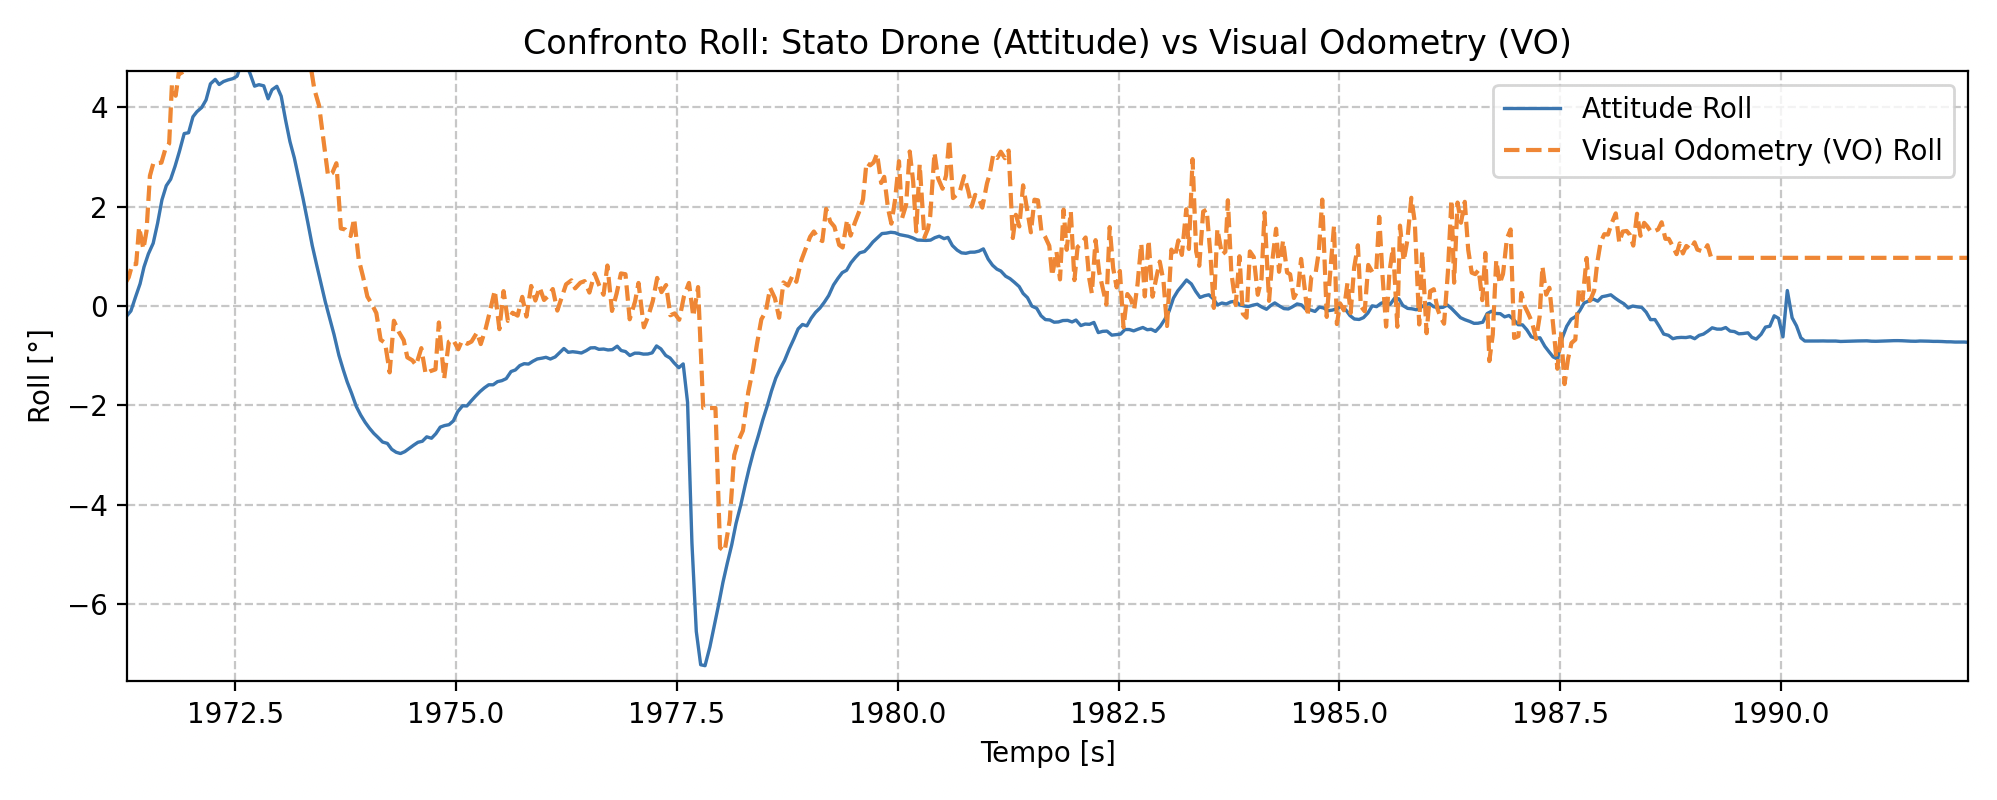
\includegraphics[width = 1\textwidth, trim={0 0 0 0}, clip]{immagini/real_probl.png}
	\caption{Grafico log di volo reale che mostra il problema del calcolo di roll e pitch con la VO.}
	\label{fig:real_probl}
\end{figure} \\
Per questo motivo è stato scelto di escludere i valori di roll e pitch dalla VO, e affidare il calcolo di questi valori all'IMU che, se correttamente calibrato, rappresenta un ottimo stimatore per questi valori; inoltre, non risulta più necessario avere la camera perfettamente perpendicolare al flight controller. Per fare ciò, basta inserire nella matrice di covarianza il valore \texttt{NaN} nelle posizioni in cui il calcolo della VO non è valido\footnote{\url{https://mavlink.io/en/messages/common.html\#ODOMETRY}}. \\ \\
Lo yaw risulta molto valido. In questo caso, è necessario che il filtro di Kalman lo elabori dato che l'IMU stima lo yaw tramite gli accellerometri; e inoltre, in questo modo lo yaw dipende dall'orientamento dei marker, non da quello iniziale del drone. Nella Fig. \ref{fig:real_yaw} è preente il grafico dello yaw di questa missione. Osservando l'asse Y, possiamo notare che lo yaw oscilla di 3-4°, valori perfettamente normali, soprattutto quando il drone è in movimento. 
\begin{figure}[!htbp]
	\centering
	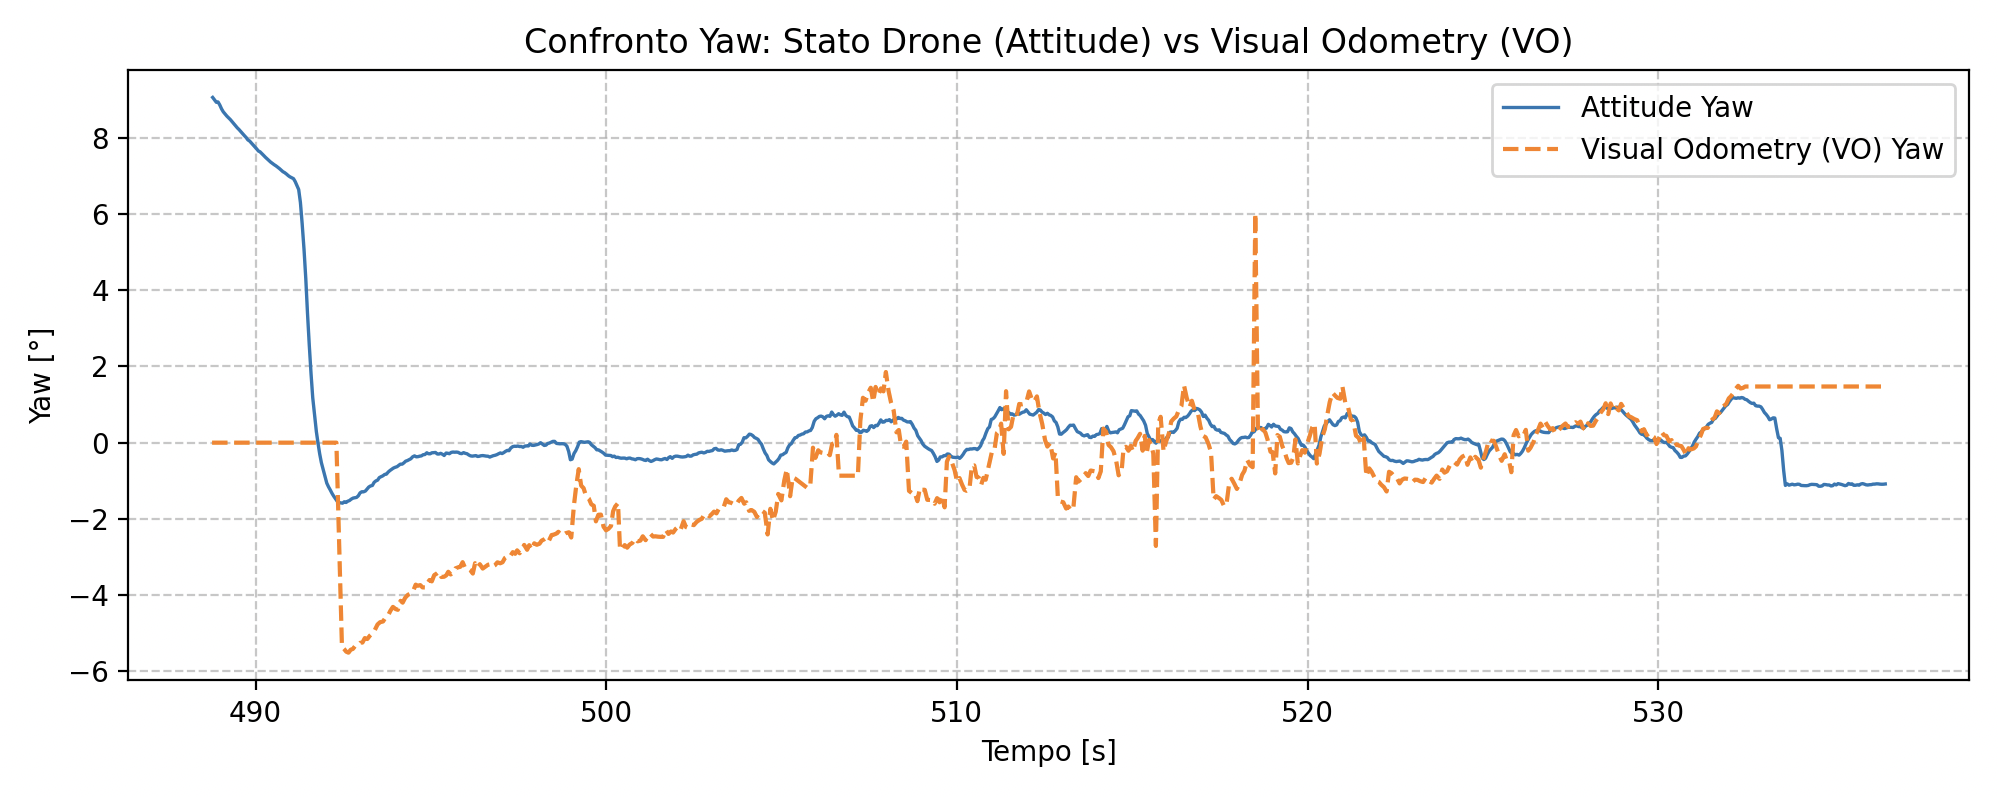
\includegraphics[width = 1\textwidth, trim={0 0 0 0}, clip]{immagini/real_yaw.png}
	\caption{Grafico log di volo reale che confronta lo yaw della VO e quello dell'IMU.}
	\label{fig:real_yaw}
\end{figure}
La Fig. \ref{fig:real_yaw2} mostra lo yaw di un volo eseguito in manuale, utilizzando sempre lo stesso sistema per la VO. Qui si può facilmente notare come entrambi i valori si comportino allo stesso modo; inoltre, al tempo 54 è presente una discontinuità dovuta dal fatto che il dominio di yaw è [-180°, 180°].
\begin{figure}[!htbp]
	\centering
	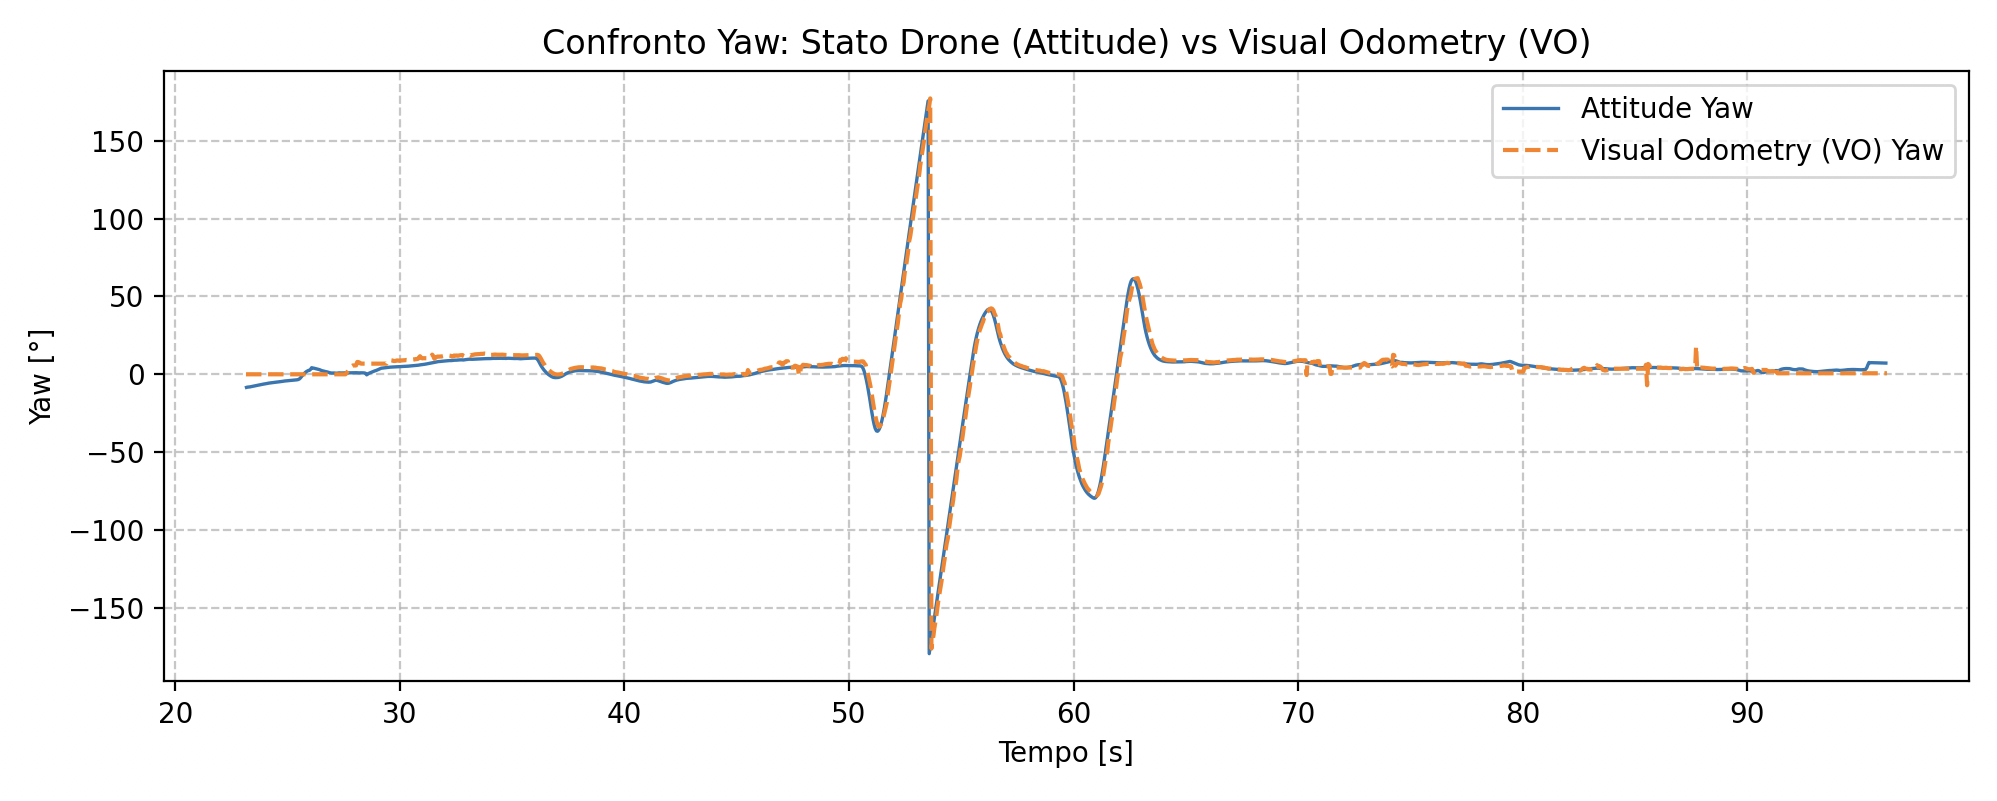
\includegraphics[width = 1\textwidth, trim={0 0 0 0}, clip]{immagini/real_yaw2.png}
	\caption{Grafico log di volo reale in modalità manuale che confronta lo yaw della VO e quello dell'IMU.}
	\label{fig:real_yaw2}
\end{figure} \\
Per quanto riguarda il calcolo della posizione, nella Fig. \ref{fig:real_xy} si può osservare come le coordinate X e Y siano ottime: il filtro di Kalman segue correttamente i dati della VO, correggendo le eventuali fluttuazioni temporanee. 
\begin{figure}[!htbp]
	\centering
	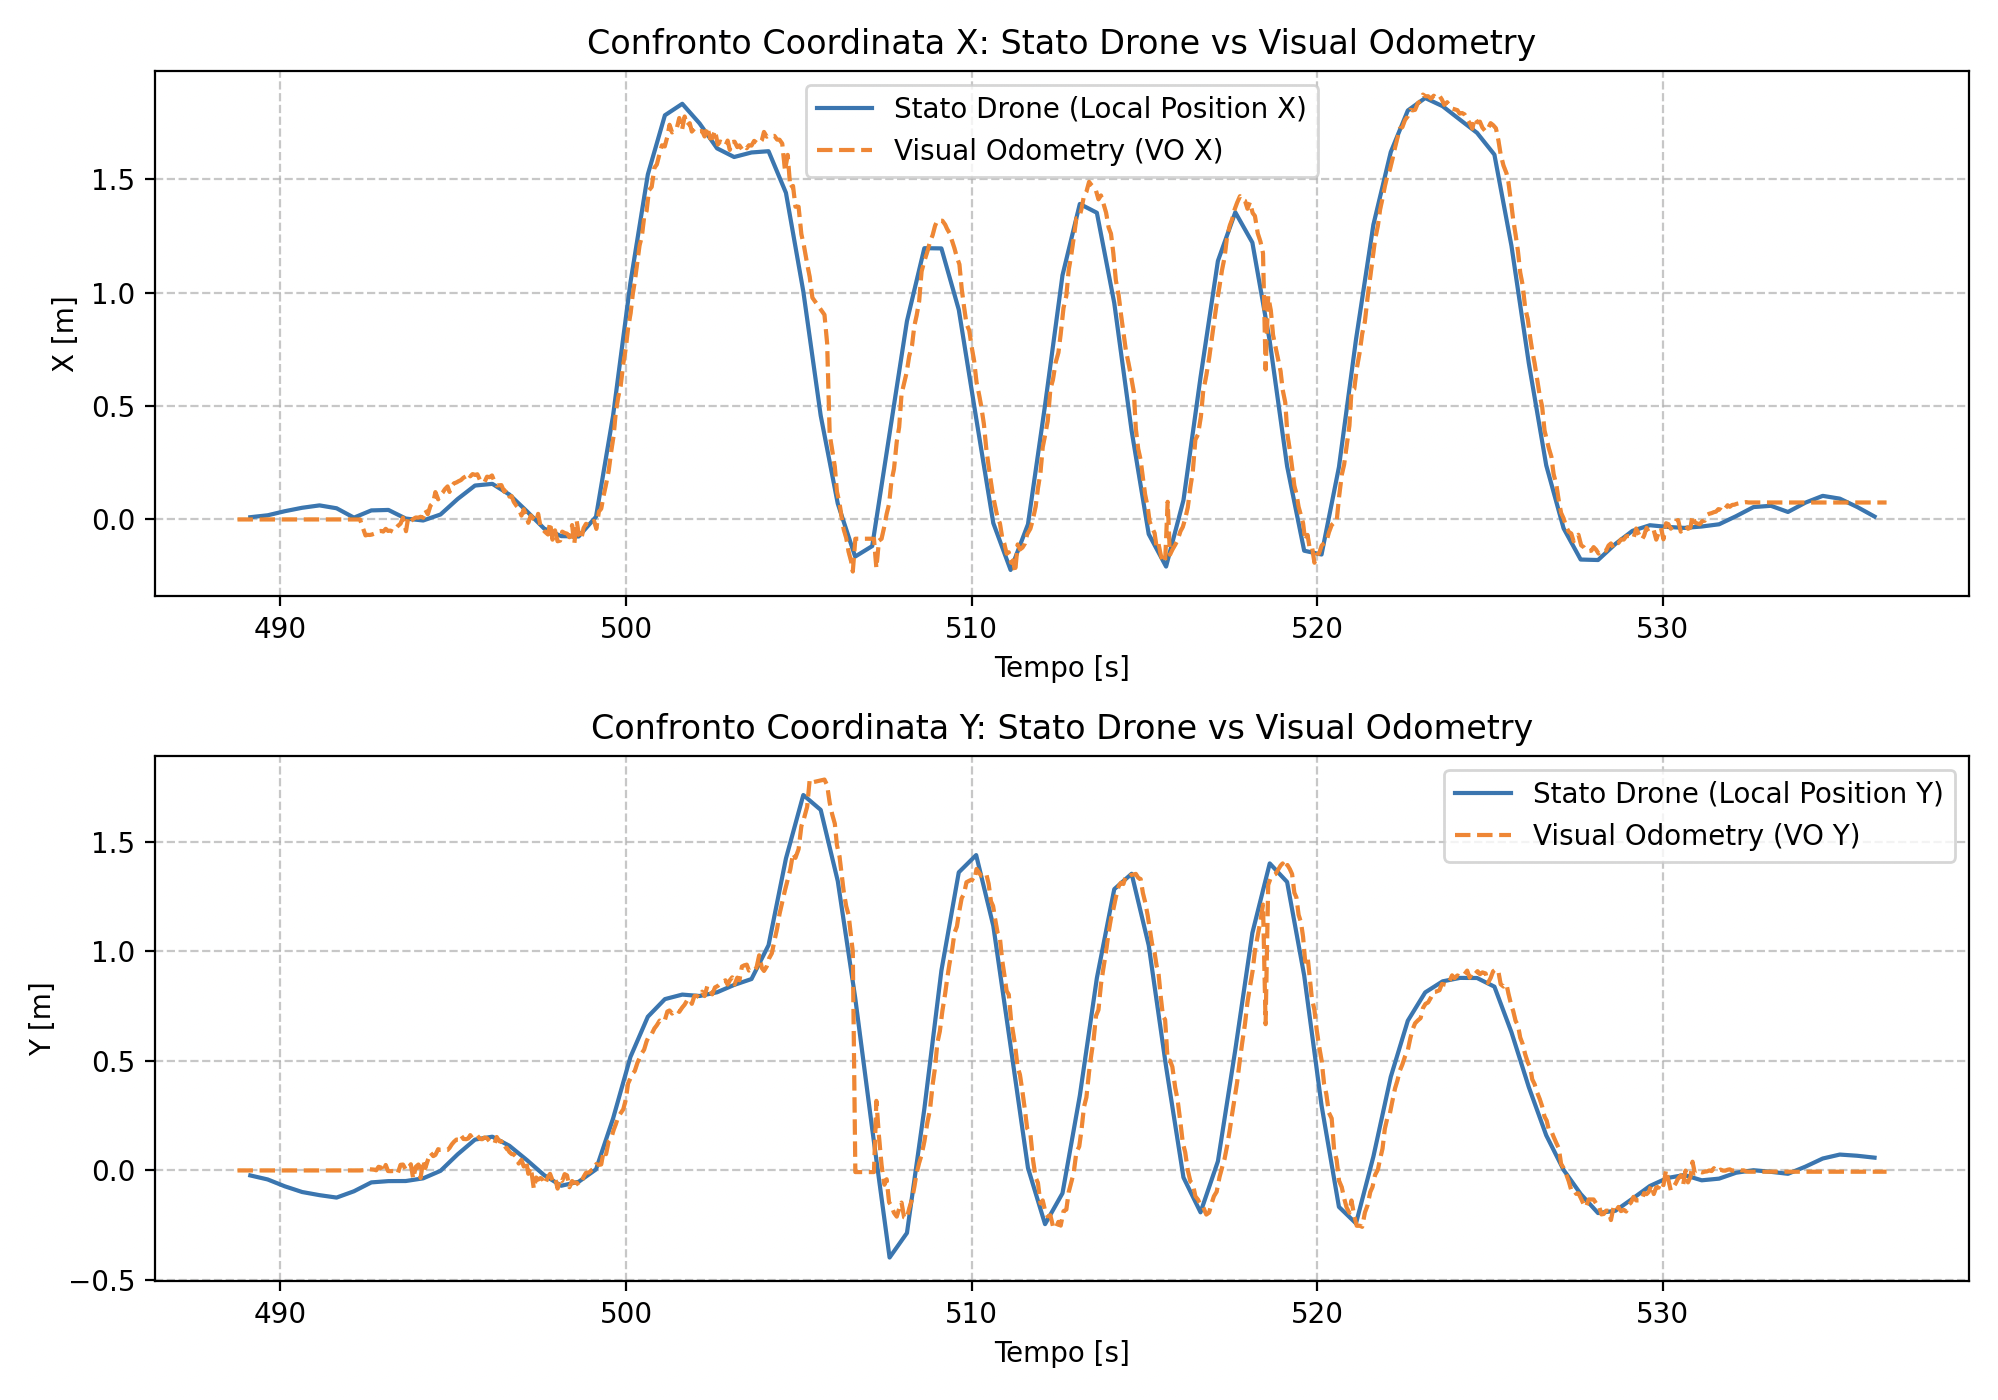
\includegraphics[width = 1\textwidth, trim={0 0 0 0}, clip]{immagini/real_xy.png}
	\caption{Grafico log di volo reale che confronta le coordinate XY della VO e lo stato nel filtro di Kalman.}
	\label{fig:real_xy}
\end{figure}
Mentre per quanto riguarda la coordinata Z (Fig. \ref{fig:real_z}), anche qui si è ottenuto un ottimo risultato. Si possono fare le stesse considerazioni fatte al simulatore per quanto riguarda il decollo/atterraggio e le oscillazioni presenti durante i movimenti del veivolo.
\begin{figure}[!htbp]
	\centering
	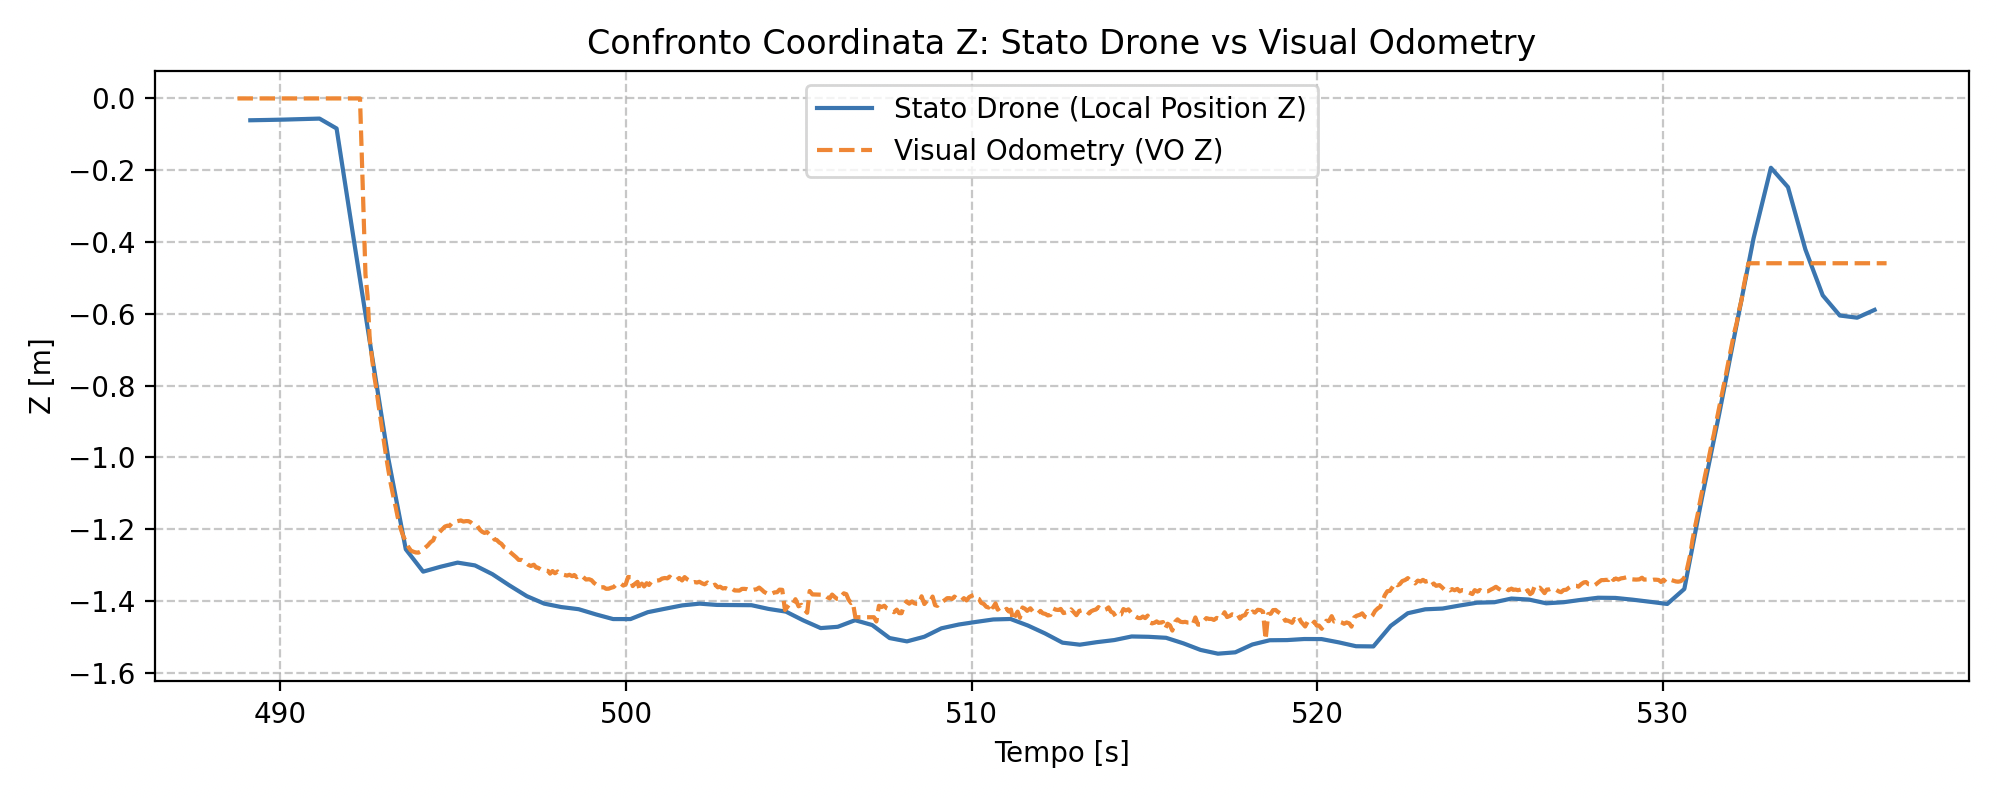
\includegraphics[width = 1\textwidth, trim={0 0 0 0}, clip]{immagini/real_z.png}
	\caption{Grafico log di volo reale che confronta la coordinata Z della VO e lo stato nel filtro di Kalman.}
	\label{fig:real_z}
\end{figure}




analisi coordinate xyz
framerate
analisi cpu, memoria,...
ci sta mettere dei paragrafi: analisi posa, analisi posizione,...

%   CAPITOLO 5: 
\chapter{Conclusione e sviluppi futuri}
\label{chap:conclusione_sviluppi_futuri}

\section{Risultati}
In questa tesi è stato sviluppato e sperimentato un sistema di navigazione autonoma per un drone in ambiente indoor, basato sull'utilizzo di marker come riferimenti per il sistema di localizzazione, in alternativa ai tradizionali sistemi di geolocalizzazione. Il sistema ha permesso di integrare un software ad hoc per l'elaborazione delle immagini sul companion computer con il firmware PX4, trasmettendo le stime di posizione e orientamento ottenute mediante visual odometry al flight controller. Inoltre è stato sviluppato un sistema per eseguire le missioni in autonomia, utilizzando la modalità Offboard di PX4.\\ \\
I test effettuati sul simulatore hanno permesso di sviluppare e verificare il corretto funzionamento del sistema di localizzazione e gestione della missione, mentre gli esperimenti condotti sul drone fisico hanno permesso di valutarne il comportamento in un ambiente reale.\\
I risultati ottenuti mostrano un sistema stabile, affidabile e preciso, soprattutto per un uso indoor.\\ \\
Le prove hanno evidenziato alcuni limiti legati alle capacità computazionali, temperature elevate e consumo della RAM del companion computer. Oltre a ciò, si potrebbe rendere il sistema ancora più preciso, soprattutto per quanto riguarda la modalità waypoint. Nonostante tali limitazioni, il sistema realizzato rappresenta una soluzione per la navigazione autonoma in assenza di geolocalizzazione e costituisce una base per ulteriori sviluppi e ottimizzazioni.

\section{Sviluppi futuri}
I risultati ottenuti, oltre a essere utili per valutare le prestazioni del sistema corrente, permettono di formulare alcune considerazioni per alcuni sviluppi futuri, con l'obiettivo di migliorare il sistema rendendolo più efficiente e affidabile.

\subsubsection{Ottimizzazione degli algoritmi per il companion computer}
Un possibile sviluppo futuro riguarda l'ottimizzazione degli algoritmi per la VO e un possibile cambiamento della piattaforma hardware utilizzata.  In questo lavoro è stato utilizzato un Raspberry Pi 3B, che permette di eseguire tutti gli algoritmi e le acquisizioni delle immagini senza particolari problemi. Tuttavia, una piattaforma più leggera, compatta ed efficiente potrebbe apportare notevoli benefici in termini di consumi energetici, di gestione della temperatura e di peso complessivo del drone, aspetti di fondamentale importanza nel campo dell'aeronautica. \\
Una soluzione molto interessante potrebbe essere l'utilizzo di un Raspberry Pi Zero 2 W\footnote{\url{https://www.raspberrypi.com/products/raspberry-pi-zero-2-w/}} combinato con un'ottimizzazione degli algoritmi per la visione artificiale, riducendo il carico computazionale richiesto per l'elaborazione delle immagini. Inoltre, sarà necessario individuare un compromesso tra prestazioni, framerate e le risorse dell'hardware, mantenendo allo stesso tempo un livello di affidabilità adeguato per il volo.

\subsubsection{Algoritmi automatici per la costruzione della mappa dei marker}
Un'altra possibile evoluzione del sistema potrebbe essere la realizzazione di un algoritmo per la costruzione automatica della mappa dei marker, evitando la necessità di inserire manualmente le coordinate di ciascun marker all'interno del sistema. \\
L'introduzione di questo algoritmo permetterebbe al sistema di individuare autonomamente la posizione dei marker presenti nell'ambiente durante la fase di esplorazione, costruendo progressivamente una mappa interna. Inoltre, l'algoritmo dovrebbe aggiornare in modo graduale le stime delle posizioni dei marker, riducendo così l'errore di localizzazione.\\
Una volta costruita, la mappa può essere memorizzata e utilizzata per le missioni successive, permettendo al drone di conoscere la propria posizione. Nella Sec. \ref{sec:problema:letteratura} sono state presentate delle possibili tecnologie utili per la realizzazione di questo algoritmo. \\
Tale funzionalità rappresenterebbe un'evoluzione del sistema, riducendone le operazioni necessarie per la sua configurazione. 


%
%			BIBLIOGRAFIA
%

% Si può specificare a che livello della TOC deve essere la bibliografia.
% Il default è 'chapter', per 'part' usare
% \beforebibliography[part]
\beforebibliography
\bibliographystyle{unsrt}
\bibliography{bibliografia}

% Pagina di chiusura
% \closingpage

\end{document}
